% arara: pdflatex: { synctex: yes }
% arara: makeindex: { style: ctuthesis }
% arara: bibtex

% The class takes all the key=value arguments that \ctusetup does,
% and a couple more: draft and oneside
\documentclass[twoside]{ctuthesis}


\usepackage[utf8]{inputenc}
\usepackage{caption}
\usepackage{subcaption}
\usepackage{tikz}
\usetikzlibrary{shapes.geometric}
\usetikzlibrary{arrows.meta,arrows}
\usepackage[demo,abs]{overpic}
% Pictures
\usepackage{graphicx,import}
\graphicspath{ {images/svg/} {images/svg/otopna-soustava/} {images/svg/software/}}
% Table
\usepackage{multirow}
\usepackage{slashbox}

\usepackage{makecell}
\renewcommand\theadfont{\bfseries}


% Notes
\usepackage{threeparttable}

% List of terms and abbreviations
\usepackage[automake,acronym,nonumberlist]{glossaries}

% Bibtex
% Zalomeni dlouheho url
\usepackage{xurl}

% Zamezeni parchantum
\usepackage{nowidow}

% Vlozeni PDF souboru
\usepackage{pdfpages}

% Balicek na posunuti cislovani stranek u PDF prilohy
\usepackage{fancyhdr}
% Importovani text souboru z podslozek
\usepackage{import}

% Rotace obrázku pro blokové schéma HA
\usepackage{rotating}
%\usepackage{tikz}




\ctusetup{
	%preprint = \ctuverlog,
%	mainlanguage = english,
	titlelanguage = czech,
	mainlanguage = czech,
	otherlanguages = {slovak,english},
	title-czech = {Systém pro podlahové vytápění rodinného domu pomocí zónové regulace},
	title-english = {System for underfloor heating of a family house using zone control},
%	subtitle-czech = {Cesta do tajů kdovíčeho},
%	subtitle-english = {Journey to the who-knows-what wondeland},
	doctype = M,
	faculty = F3,
	department-czech = {Katedra mikroelektroniky},
	department-english = {Department of Microelectronics},
	author = {Bc. Roman Labovský},
	supervisor = {Ing. Vladimír Janíček, Ph.D.},
	supervisor-address = {České vysoké učení technické v Praze, Fakulta elektrotechnická, Katedra mikroelektroniky\\ Technická 2, \\ Praha 6 \\ 166 27},
%	supervisor-specialist = {John Doe},
	fieldofstudy-english = {Electronics},
	subfieldofstudy-english = {Electronics and Communication},
	fieldofstudy-czech = {Elektronika},
	subfieldofstudy-czech = {Elektronika a komunikace},
	keywords-czech = {termostat, Home Assistant, zónová regulace vytápění, podlahové vytápění, Power over Ethernet, ESP32 },
	keywords-english = {thermostat, Home Assistant, zone heating control, underfloor heating, Power over Ethernet, ESP32},
	day = 3,
	month = 1,
	year = 2022,
	specification-file = {zadani-dp.pdf},
	front-specification = true,
%	front-list-of-figures = false,
%	front-list-of-tables = false,
%	monochrome = true,
%	layout-short = true,
	pkg-listings = true,
}

\ctuprocess

\addto\ctucaptionsczech{%
	\def\supervisorname{Vedoucí}%
	\def\subfieldofstudyname{Studijní program}%
}

\ctutemplateset{maketitle twocolumn default}{
	\begin{twocolumnfrontmatterpage}	
		\ctutemplate{twocolumn.thanks}
		\ctutemplate{twocolumn.declaration}
		\ctutemplate{twocolumn.abstract.in.titlelanguage}
		\ctutemplate{twocolumn.abstract.in.secondlanguage}
		\ctutemplate{twocolumn.tableofcontents}
		\ctutemplate{twocolumn.listoffigures}
	\end{twocolumnfrontmatterpage}
}

% Posunuti cislovani stranky dolu u vlozenych PDF (priloha)
\fancypagestyle{includedpages}{%
  \fancyhf{}%
  \renewcommand{\headrulewidth}{0pt}%
  \setlength{\footskip}{70pt}
  \fancyfoot[C]{\thepage}%
}

% Seznam prilohy
\newcommand\listappendixname{Seznam příloh}
\newcommand\appcaption[1]{%
   \addcontentsline{app}{chapter}{#1}}
\makeatletter
\newcommand\listofappendices{%
   \section*{\listappendixname}\@starttoc{app}}

% Diakritika pro listings (zapis kodu)
\lstset{
     literate=%
         {á}{{\'a}}1
         {í}{{\'i}}1
         {é}{{\'e}}1
         {ý}{{\'y}}1
         {ú}{{\'u}}1
         {ó}{{\'o}}1
         {ě}{{\v{e}}}1
         {š}{{\v{s}}}1
         {č}{{\v{c}}}1
         {ř}{{\v{r}}}1
         {ž}{{\v{z}}}1
         {ď}{{\v{d}}}1
         {ť}{{\v{t}}}1
         {ň}{{\v{n}}}1                
         {ů}{{\r{u}}}1
         {Á}{{\'A}}1
         {Í}{{\'I}}1
         {É}{{\'E}}1
         {Ý}{{\'Y}}1
         {Ú}{{\'U}}1
         {Ó}{{\'O}}1
         {Ě}{{\v{E}}}1
         {Š}{{\v{S}}}1
         {Č}{{\v{C}}}1
         {Ř}{{\v{R}}}1
         {Ž}{{\v{Z}}}1
         {Ď}{{\v{D}}}1
         {Ť}{{\v{T}}}1
         {Ň}{{\v{N}}}1                
         {Ů}{{\r{U}}}1    
}

% Theorem declarations, this is the reasonable default, anybody can do what they wish.
% If you prefer theorems in italics rather than slanted, use \theoremstyle{plainit}
\theoremstyle{plain}
\newtheorem{theorem}{Theorem}[chapter]
\newtheorem{corollary}[theorem]{Corollary}
\newtheorem{lemma}[theorem]{Lemma}
\newtheorem{proposition}[theorem]{Proposition}

\theoremstyle{definition}
\newtheorem{definition}[theorem]{Definition}
%\newtheorem{example}[theorem]{Example}
\newtheorem{conjecture}[theorem]{Conjecture}

\theoremstyle{note}
\newtheorem*{remark*}{Remark}
\newtheorem{remark}[theorem]{Remark}
% Velikost mezery mezi odstavci
\setlength{\parskip}{2.5ex plus 0.2ex minus 0.2ex}

% Abstract in Czech
\begin{abstract-czech}
Tato diplomová práce se zabývá problematikou regulace zónového podlahového vytápění rodinného domu. Pro řízení se využívá systém Home Assistant fungující na Raspberry Pi, který je ovladatelný přes webové rozhraní. V~rámci systému jsou vybraná nebo zhotovená zařízení pro ovládání jednotlivých částí zónové regulace vytápění a lokální snímače prostorové teploty. Následně je celý řídicí systém testován a používán v reálném prostředí.
\end{abstract-czech}

% Abstract in English
\begin{abstract-english}
This thesis deals with a system for regulation of zone heating of family house. Proposed control system is based on Raspberry Pi with the Home Assistant system. The unit is fully controllable via web. Devices for controlling individual parts of the heating zone control and local room temperature sensors were selected or made within the system.  The programmed system was eventually tested in real environment.
\end{abstract-english}

% Acknowledgements / Podekovani
\begin{thanks}
V prvé řadě bych chtěl poděkovat svému vedoucímu Ing. Vladimíru Janíčkovi, Ph.D. za odborné vedení práce, věcné připomínky a~vstřícnost při konzultacích.

Dále bych chtěl poděkovat svému kamarádovi Ing. Tomáši Janouškovi a jeho rodině za možnost aplikovat svou práci na jejich rodinném domě a především za trpělivost během nasazování systému.

Děkuji studentskému klubu Silicon Hill a~projektu „MacGyver – Bastlíři SH“ za umožnění přístupu k měřicímu vybavení, pájecí a~osazovací technice.
\end{thanks}

% Declaration / Prohlaseni
\begin{declaration}
Prohlašuji, že jsem předloženou práci vypracoval samostatně a že jsem uvedl veškeré použité informační zdroje v souladu s Metodickým pokynem o dodržování etických principů při přípravě vysokoškolských závěrečných prací.


V Praze, \ctufield{day}.~\monthinlanguage{title}~\ctufield{year}

% Podpis pod prohlasenim
\begin{flushright}
	\parbox{5cm}
	{
		\begin{center}
			\dotfill \\ Bc. Roman Labovský
		\end{center}
	}
\end{flushright}
\end{declaration}

% Only for testing purposes
\listfiles
\usepackage[pagewise]{lineno}
\usepackage{lipsum,blindtext}
\usepackage{mathrsfs} % provides \mathscr used in the ridiculous examples



\newacronym{mqtt}{MQTT}{Message Queuing Telemetry Transport}
\newacronym{usb}{USB}{Universal Serial Bus}
\newacronym{i2c}{I$^2$C}{Inter-Integrated Circuit}
\newacronym{ram}{RAM}{Random Access Memory}
\newacronym{led}{LED}{Light-Emitting Diode}
\newacronym{lcd}{LCD}{Liquid Crystal Display}
\newacronym{pwm}{PWM}{Pulse Width Modulation}
\newacronym{poe}{POE}{Power Over Ethernet}
\newacronym{m2m}{M2M}{Machine To Machine}
\newacronym{json}{JSON}{JavaScript Object Notation}
\newacronym{bjson}{BJSON}{Binary JavaScript Object Notation}
\newacronym{tcp/ip}{TCP/IP}{Transmission Control Protocol/Internet Protocol}
\newacronym{qos}{QoS}{Quality of Service}
\newacronym{ssl}{SSL}{Secure Sockets Layer}
\newacronym{tls}{TLS}{Transport Layer Security}
\newacronym{scl}{SCL}{Synchronous Clock}
\newacronym{sda}{SDA}{Synchronous Data}
\newacronym{rom}{ROM}{Read Only Memory}
\newacronym{api}{API}{Application Programming Interface}
\newacronym{ha}{HA}{Home Assistant}
\newacronym{lan}{LAN}{Local Area Network}

\newacronym{tuv}{TUV}{Teplá užitková voda}
\newacronym{dps}{DPS}{Deska plošných spojů}
\newacronym{nc}{NC}{Normally Closed}


\newacronym{pse}{PSE}{Power Sourcing Equipment}
\newacronym{pd}{PD}{Powered Device}
\newacronym{ldo}{LDO}{Low-dropout regulator}
\newacronym{rmii}{RMII}{Reduced Media­-Independent Interface}
\newacronym{pet-g}{PET-G}{Polyethylentereftalát, „G“ znamená modifikovaný glykol}
\newacronym{dtr}{DTR}{Data Terminal Ready}
\newacronym{rts}{RTS}{Request To Send}
\newacronym{yaml}{YAML}{YAML Ain't Markup Language }
\newacronym{esd}{ESD}{Electrostatic discharge}

\newacronym{utp}{UTP}{Unshielded Twisted Pair}
\newacronym{uart}{UART}{Universal Asynchronous Receiver-Transmitter}
\newacronym{tvs}{TVS}{Transient Voltage Suppressor}
\newacronym{ptc}{PTC}{Positive Temperature Coefficient}
\newacronym{ntc}{NTC}{Negative Temperature Coefficient}

\newacronym{zov}{ZOV}{Zásobník otopné vody}
\newacronym{nspt}{NSPT}{Nástěnný snímač prostorové teploty}




\makeglossaries
\renewcommand{\acronymname}{Seznam použitých zkratek a symbolů}

% Redukovani automaticky mezer mezi odstavci
\clubpenalty=10000
\widowpenalty=10000
\raggedbottom

% PDF informace
\hypersetup{pdfauthor   = Roman Labovský,
            pdftitle    = Systém pro podlahové vytápění rodinného domu pomocí zónové regulace,
            pdfsubject  = Diplomová práce,
            pdfkeywords = {termostat, Home Assistant, zónová regulace vytápění, podlahové vytápění, Power over Ethernet, ESP32},
            pdfproducer = Texmaker 5.0.4,
            pdfcreator  = LaTeX editor}

\begin{document}

\maketitle

\printglossaries


\chapter{Úvod}

V současné době s rozvojem elektroniky jsou k dipozici nové možnosti domácí automatizace různého druhu. Cílem této automatizace je ekonomické, energetické řízení, víceúčelové použití a rekonfigurace nastavení a to vše pro potřeby obyvatel s cílem zvýšit jejich pohodlí.


Jednou ze zajímavých oblastí této automatizace je vytápění domácnosti. Na dnešním trhu je možné nalézt mnoho výrobců tohoto řešení. Všichni však mají stejný primární cíl dosáhnout požadované teploty v místnosti, co možná s největšími úspory na spotřebované energii. To ve většině případech dosahují podle nastaveného teplotního režimu od uživatele. Existují i~takové, které si tento režim udělají sami podle aktivit obyvatel. Vzhledem k~budování nízkoenergetický, pasivních či nulových domů je optimální vytápění nezbytností.

Jako další alternativa pro řešení oblasti vytápění domácnosti vznikla tato práce. Podobnou tématikou jsem se zabýval i ve své bakalářské práci. Kde jsem automatizaci vytápění aplikoval na starším rodinném domě s centrálním termostatem, automatickým peletovým kotlem, deskovými otopnými tělesy a~se zásobníkem teplé užitkové vody. V diplomové práci využívám stejný řídicí software pro vytápění, ale jedná se o novostavbu s podlahovým vytápěním, zónovou regulací, centrálním zásobník otopné vody (se zabudovaným zásobníkem teplé užitkové vody). Jako zdroje tepla jsou použity krby s teplovodním výměníkem a plynový kondenzační kotel.

Současná verze dokumentu je charakteru semestrálního projektu, která je teoretickým podkladem k diplomové práci a bude její součástí. Cíle tohoto semestrálního projektu jsou popsány níže. Práce je nyní rozdělena na tři části. V~první části jsou uvedeny informace o podlahovém vytápění a komerčních produktech. V druhé části se zabývám hardwarovým konceptem celého řídicího systému a nutných zařízení pro zónovou regulaci vytápění. V poslední třetí části se věnuji komunikační části mezi centrální jednotkou a akčními členy pro řízení jednotlivých topných okruhů.

\section{Cíl práce}
\begin{itemize}
\item Prostudujte problematiku podlahového vytápění při využití zónové regulace a její principy.
\item Navrhněte koncept centrální jednotky a dalších nutných zařízení pro zónovou regulace vytápění.
\item Navrhněte koncept komunikace centrální jednotky, lokálních nástěnných snímačů prostorové teploty a akčních členů pro řízení jednotlivých topných okruhů.
\item Vyberte nebo zhotovte zařízení pro ovládání jednotlivých částí zónové regulace vytápění a lokální snímače prostorové teploty.
\item V řídícím systému využijte inteligentní část pro vytápění.
\item Ověřte funkčnost celého systému. Navrhněte případná vylepšení.

\end{itemize}


%!TEX ROOT=ctutest.tex

\chapter{Rešerše}


\section{Podlahové vytápění}

U podlahového vytápění dochází k přenosu tepla do vytápěného prostoru převážně sáláním. Což má za následek, že se od sálající plochy ohřívají plochy osálané a teprve od sálajících a osálaných ploch se ohřívá okolní vzduch (druhá konvenkční složka z celkového tepelného toku). Naproti tomu při přenosu tepla pomocí deskových/článkových/trubkových otopných těles či konvektory dochází k přenosu pomocí proudění (konvekční složka). 
Teplota otopné plochy je poměrně nízká pohybuje se mezi 25 až 34~°C u podlahového vytápění a tedy i teplota teplonosné látky je nízká (otopná plocha je zahřívaná buď teplou vodou, teplým vzduchem nebo elektricky). Proto je tento typ vytápění vhodné využít při zapojení s nízkoteplotním zdrojem, jako jsou tepelná čerpadla, kondenzační kotle či solární panely.

Důležitým parametrem pro příjemný pobyt v místnosti je prostorové rozložení teploty, jak ve vertikální tak horizontální rovině. Na vertikální rozložení teplot ve vytápěné místnosti je způsobeno nerovnoměrným přívodem tepla a nerovnoměrným ochlazování jednotlivých stěn místnosti. Vertikální nerovnoměrnost teplot je tím větší, čím vyšší je povrchová teplota otopné plochy. Vzhledem k tomu, že teplota u podlahové vytápění je povrchová teplota otopné vody ze všech druhů velkoplošného vytápění (podlahové, stropní, stěnové) nejnižší, je vertikální rozložení teplot skoro ideální, viz obrázek \ref{fig:vertikalni-prubehy-teplot-pro-ruzne-druhy-vytapeni}a. Optimální vytápění by mělo zajistit, aby v oblasti hlavy stojícího člověka byla teplota minimálně o 2 °C nižší, než je v úrovni kotníků. Takovému ideálnímu průběhu teplot odpovídá obrázek \ref{fig:vertikalni-prubehy-teplot-pro-ruzne-druhy-vytapeni}b. Dále jsou na obrázku  \ref{fig:vertikalni-prubehy-teplot-pro-ruzne-druhy-vytapeni} další způsoby vytápění s vertikálními průběhy teplot. Na obrázku \ref{fig:porovnani-rozlozeni-teplot} je prostorové porovnání teplot podlahové vytápění a vytápění při využití deskových/článkových otopných těles s~vyznačenými oblastmi teplot.


\begin{figure}[h]

\centering
\begin{picture}(370,150)
\put(0,0){\includegraphics[width=\textwidth]{images/vertikalni-prubehy-teplot-pro-ruzne-druhy-vytapeni.png}}
\put(5,6){\scriptsize \sffamily Rostoucí teplota}
\put(161,6){\scriptsize \sffamily Klesající teplota}
\put(19,31){\scriptsize \sffamily t[°C]}
\put(15,132){\scriptsize \sffamily h[cm]}
\put(22,41){\fontsize{6}{6} \sffamily Podlaha}
\put(22,141){\fontsize{6}{6} \sffamily Strop}
\put(50,41){\scriptsize \sffamily 0}
\put(40,104){\scriptsize \sffamily 170}
\put(40,132){\scriptsize \sffamily 270}

\put(84,143){\scriptsize \sffamily a)}
\put(67,33){\fontsize{5}{5} \sffamily 16}
\put(74,33){\fontsize{5}{5} \sffamily 18}
\put(81,33){\fontsize{5}{5} \sffamily 20}
\put(88,33){\fontsize{5}{5} \sffamily 22}
\put(95,33){\fontsize{5}{5} \sffamily 24}

\put(134,143){\scriptsize \sffamily b)}
\put(117,33){\fontsize{5}{5} \sffamily 16}
\put(124,33){\fontsize{5}{5} \sffamily 18}
\put(131,33){\fontsize{5}{5} \sffamily 20}
\put(138,33){\fontsize{5}{5} \sffamily 22}
\put(145,33){\fontsize{5}{5} \sffamily 24}

\put(184,143){\scriptsize \sffamily c)}
\put(167,33){\fontsize{5}{5} \sffamily 16}
\put(174,33){\fontsize{5}{5} \sffamily 18}
\put(181,33){\fontsize{5}{5} \sffamily 20}
\put(188,33){\fontsize{5}{5} \sffamily 22}
\put(195,33){\fontsize{5}{5} \sffamily 24}

\put(234,143){\scriptsize \sffamily d)}
\put(217,33){\fontsize{5}{5} \sffamily 16}
\put(224,33){\fontsize{5}{5} \sffamily 18}
\put(231,33){\fontsize{5}{5} \sffamily 20}
\put(238,33){\fontsize{5}{5} \sffamily 22}
\put(245,33){\fontsize{5}{5} \sffamily 24}

\put(284,143){\scriptsize \sffamily e)}
\put(267,33){\fontsize{5}{5} \sffamily 16}
\put(274,33){\fontsize{5}{5} \sffamily 18}
\put(281,33){\fontsize{5}{5} \sffamily 20}
\put(288,33){\fontsize{5}{5} \sffamily 22}
\put(295,33){\fontsize{5}{5} \sffamily 24}

\put(334,143){\scriptsize \sffamily f)}
\put(317,33){\fontsize{5}{5} \sffamily 16}
\put(324,33){\fontsize{5}{5} \sffamily 18}
\put(331,33){\fontsize{5}{5} \sffamily 20}
\put(338,33){\fontsize{5}{5} \sffamily 22}
\put(345,33){\fontsize{5}{5} \sffamily 24}
\end{picture}
	 \caption[Vertikální průběh teploty vzduchu u podlahové vytápění.]{Vertikální průběh teploty vzduchu ve vytápěné místnosti při různém způsobu vytápění. \\ a) Ideální požadovaný průběh. b) Podlahové vytápění. c) Vytápění deskovými/článkovými otopnými tělesy (vnitřní stěna). d) Vytápění deskovými/článkovými otopnými tělesy (venkovní stěna). e) Konvektory. f) Stropní vytápění. Upraveno z \cite{vertikalni-prubehy-teplot-pro-ruzne-druhy-vytapeni}. }
	 \label{fig:vertikalni-prubehy-teplot-pro-ruzne-druhy-vytapeni}
\end{figure}

\hspace{5mm}

  \begin{figure}[H]
     \subfloat[Rozložení teplot při použití podlahové vytápění.\label{fig:rozlozeni-teplot-podlahove-vytapeni}]{
       \begin{overpic}[width=0.5\textwidth]{images/rozlozeni-teplot-podlahove-vytapeni.png}
         \put(20,10){\scriptsize \sffamily 22 °C}
         \put(65,50){\scriptsize \sffamily 20 °C}
         \put(8,115){\scriptsize \sffamily 17 °C}
         \put(155,90){\scriptsize \sffamily 18 °C}
       \end{overpic}
     }
     \subfloat[Rozložení teplot při použití deskových/článkových otopných těles. \label{fig:rozlozeni-teplot-radiatory}]{
       \begin{overpic}[width=0.5\textwidth]{images/rozlozeni-teplot-radiatory.png}
         \put(20,10){\scriptsize \sffamily 14 °C}
         \put(100,15){\scriptsize \sffamily 33 °C}
         \put(133,37){\scriptsize \sffamily 37 °C}
         \put(32,50){\scriptsize \sffamily 22 °C}
         \put(113,77){\scriptsize \sffamily 30 °C}
         \put(20,87){\scriptsize \sffamily 19 °C}
         \put(160,95){\scriptsize \sffamily 20 °C}
         \put(42,117){\scriptsize \sffamily 23 °C}
       \end{overpic}
     }
     \caption[Porovnání rozložení teplot při použití podlahové vytápění a deskových/článkových otopných těles.]{Porovnání rozložení teplot při použití podlahové vytápění a deskových/článkových otopných těles. Upraveno z \cite{rozlozeni-teplot-podlahove-vytapeni-a-radiatory}.}\label{fig:porovnani-rozlozeni-teplot}
   \end{figure}
   


\subsubsection{Výhody}

\begin{itemize}
  \item Je vhodné zejména tam, kde je nízkoteplotní zdroj tepla (tepelné čerpadlo, kondenzační kotel, solární panely, …).
  \item Větší užitný prostor (místo nezabírají otopná tělesa).
  \item Cirkulace vzduchu je nižší oproti deskovým/článkovým otopným tělesům, proto je víření prachu v~místnosti menší.
  \item Téměř rovnoměrná teplota místnosti.
\end{itemize}

\subsubsection{Nevýhody}

\begin{itemize}
  \item Zvýšené náklady na realizaci.
  \item Nezbytná pečlivá montáž a stavební dozor.
  \item Vyšší tepelná setrvačnost otopné soustavy.
  \item Vyšší nároky na řízení podlahové otopné plochy (zejména hlídání maximální vstupní otopné vody).
\end{itemize}

\section{Zónová regulace vytápění}

Význam zónové regulace vytápění spočívá v systému umožňující individuální vytápění v~jednotlivých místnostech (každá místnost nebo spojení více místností se označuje za zónu) na požadovanou teplotu.  Základ zónové regulace je centrální řídicí jednotka, která přijímá data od jednotlivých místností (zejména jejich aktuální teplotu) a dává povely do zařízení, které ovládá (otevírání/zavírání pohonů u jednotlivých otopných okruhů apod.). Přístup k~řídicí jednotce je nejčastěji pomocí displeje, webového rozhraní nebo jejich kombinace. V řídicí jednotce se dá celý systém vytápění nastavit (nastavení časových a teplotních programů pro jednotlivé zóny a mnohé další). 

Zónové systémy vytápění se rozdělují na dvě hlavní skupiny. První tvoří zónové systémy propojené pomocí vodičů a druhou skupinu tvoří bezdrátová technologie propojující centrální řídicí jednotku a jednotlivé zóny. 

Hlavní částí zónového systému je centrální řídící jednotka. Mezi další komponenty patří, nástěnné snímače vnitřní teploty, snímač venkovní teploty, termoelektrické pohony, elektronické regulátory otopných těles, reléová spínací jednotka. Mezi komponenty, které přispívají ke komfortu zónové regulace jako senzor intenzity slunečního záření, senzor rychlosti větru, různé spínací jednotky, jednotky pro ovládání žaluzií, moduly pro dálkové ovládání pomocí GSM a další.

\subsection{Principy zónové regulace vytápění}

Jak již bylo řečeno, základem celého systému je centrální řídicí jednotka. Další důležitou částí je zónový regulátor, který slouží pro ovládání komponentů, které jsou k zónovému regulátoru připojeny. Mezi hlavní komponenty, který zónový regulátor ovládá, jsou termoelektrické pohony. Termoelektrický pohon je podobný termostatické hlavici, která se nasazuje na deskové/článkové otopné těleso, ale je jej možné ovládat elektrickým napětím. Samotná regulace vytápění probíhá tak, že řídicí jednotka je propojena se zónovým regulátorem. K~zónovému regulátoru jsou připojeny jednotlivé nástěnné snímače prostorové teploty a termoelektrické pohony, které jsou nasazeny na termostatický ventilech otopných okruhů/těles. V centrální jednotce jsou nastaveny časové programy (různé požadované teploty pro různé časové úseky). Centrální jednotka posílá do zónového regulátoru požadované teploty pro všechny zóny. Tyto  teploty jsou v zónovém regulátoru porovnávány s aktuálními prostorovými teplotami měřenými nástěnnými jednotkami. V případě, že je prostorová teplota příslušné zóny nižší než požadovaná teplota (nastavená v centrální jednotce), ovládá zónový regulátor odpovídající pohon, který otevírá/zavírá daný ventil a umožňuje proudění otopné vody do otopného okruhu/tělesa, čím dochází ke změně teploty v místnosti. Pokud je připojen například kotel, je pak hořák kotle ovládán při požadavku vytápění v jakékoliv místnosti. Princip zónové regulace je zobrazen na obrázku \ref{fig:obecny-princip-zonove-regulace}.

Další možné zapojení může být takové, že jednotlivé nástěnné snímače prostorové teploty jsou přímo propojeny s centrální jednotkou, která následně podle časového programu posílá zónovému regulátoru požadavky na ovládání jednotlivých pohonů. 

\newpage
\begin{figure}[H]
    \centering
    \def\svgwidth{\columnwidth}
    \input{images/svg/obecny-princip-zonove-regulace.pdf_tex}
    \caption{Obecný princip zónové regulace vytápění.}
    \label{fig:obecny-princip-zonove-regulace}
\end{figure}

Mezi další ovládána zařízení při regulaci vytápění mohou být čerpadla, směšovací ventily zejména pro podlahové vytápění, kde je nutné udržovat teplotu otopné vody v daných mezích.

\subsection{Dostupné komerční řešení zónové regulace podlahového vytápění}

Optimální systém pro otopnou soustavu, kterou hodlám řídit z obrázku~\ref{fig:otopna-soustava-rez-domu}, se skládá z řízení ovládání kotle, spínání čerpadel v případě zatopení v~krbech a~následnou indikaci uživateli, jak je moc zásobník otopné vody naakumulovaný, dále z jednotlivých otopných okruhů (12 pohonů pro 9 zón) a~čerpadla podlahového vytápění. Pro zónovou regulaci se používá pouze patro.

\subsubsection{Elektrobock}
Česká firma Elektrobock nabízí bezdrátové řešení pro řízení podlahové vytápění. Systém řízení je zastřešené pod aplikaci PocketHome. Jednotlivé zařízení mohou fungovat samostatně bez nebo s centrální řídicí jednotkou. Tato centrální jednotka je zastřešené pod aplikaci PocketHome. Řídicí systém se skládá z centrální jednotky, nástěnných snímačů prostorové teploty pro jednotlivé místnosti a zónového regulátoru pro ovládání jednotlivých otopných okruhů (celkově je možné ovládat 9 zón) a oběhového čerpadla, dále je k dispozici zařízení pro zapínání/vypínání kotle nebo komunikace pomocí protokolu OpenTherm. Na obrázku \ref{fig:elektrobock-pocket-home} jsou zobrazena jednotlivá zařízení. Jistou nevýhodou může být bezdrátová komunikace na frekvenci 433,92 MHz, v případě delší vzdálenosti a především umístění na jiném patře centrální jednotky a nástěnných snímačů prostorové teploty, zónového regulátoru. Může docházet k problémům s komunikací, zejména pokud se jedná o~zástavbu z železobetonu, kde odrazivost a neprůchodnost signálu je poměrně značná. Jednotlivé prvky mohou pracovat samostatně bez centrální jednotky, na druhou stranu se tímto ztrácí přehled o celém systému a komfortu nastavování z jednoho místa. Systém se může spravovat pomocí PC (systém Windows) nebo pomocí chytrého telefonu/tabletu (systém Android, iOS). Systém počítá s jedním zdrojem tepla, tedy kotlem (elektrickým, plynovým, automatickým), neuvažuje se s otopnou soustavu, kde je začleněn např. krb s~tepelným výměníkem, jak z pohledu řízení čerpadel, tak i případnou indikaci o stavu naakumulovaní zásobníku s otopnou vodou. Problém bezdrátového, bateriového řešení je nutná výměna baterií po určité době.


\begin{figure}[H]

\centering
\begin{picture}(370,236)
\put(0,0){\includegraphics[width=\textwidth]{images/komercni-systemy/elektrobock-pocket-home/elektrobock-pocket-home.png}}
\put(50,226){\scriptsize \sffamily a)}
\put(180,190){\scriptsize \sffamily b)}
\put(305,235){\scriptsize \sffamily c)}
\put(180,8){\scriptsize \sffamily d)}
	 \caption[Jednotlivá zařízení systému Elektrobock PocketHome.]{Jednotlivá zařízení systému Elektrobock PocketHome. \\ 
	 a) Nástěnný snímač prostorové teploty. b) Centrální jednotka. c) Spínací jednotka kotle. d) Zónový regulátor. Upraveno z \cite{elektrobock-lokalni-termostat, elektrobock-centralni-jednotka, elektrobock-spinaci-jednotka-kotle, elektrobock-zonovy-regulator}.}
	 \label{fig:elektrobock-pocket-home}
\end{picture}

\end{figure}

\subsubsection{Honeywell}
Honeywell nabízí bezdrátový systém regulace podlahové vytápění. Systém řízení je zastřešené pod aplikaci Evohome. Skládá se z centrální jednotky s~dotykovým displejem, nástěnných snímačů prostorové teploty pro jednotlivé místnosti, zónového regulátoru pro ovládání jednotlivých otopných okruhů (celkově je možné ovládat 5 zón, s rozšiřovacím modulem je možné se dostat na 8 zón). Systém je možné rozšířit o dobíjení \acrshort{tuv} (\textit{\acrlong{tuv}}), pro sledování teploty na zásobníku je možné umístit teplotní čidlo, ze kterého je teplota odesílaná do centrální jednotky. Na obrázku \ref{fig:honeywell-evohome} jsou zobrazena jednotlivá zařízení systému. Systém však při dobíjení zásobníku TUV počítá se zdrojem tepla pouze s kotlem, takže v případě využití krbů s výměníkem nastává problém. V neposlední řadě umožňuje zapojit směšovací ventil pro optimální teplotu do podlahového topení. Systém je možné ovládat lokálně nebo řídit vzdáleně odkudkoliv, je zapotřebí zaregistrovat si účet a spárovat ho s  centrální jednotkou. Vzdálený server přijímá požadavky na změny režimů či nastavení teplot, a zasílá je do řídící jednotky. Server průběžně shromažďuje různá data o chování soustavy, a může je na základě žádosti poskytnout. Z~toho vyplývá, že pro lepší řízení a nastavení vytápění je nutné zřídit vzdálený přístup a samotné vyhodnocení a dání povelů, pak dochází na vzdálením serveru, nemáme moc pod kontrolou data a životnost takového systému do budoucnosti. Otázka je i při využití pouze lokálního režimu, zda regulace nepřichází o~výhody cloudového řešení. Problém bezdrátového řešení může být opět prostup signálu mezi zařízeními a centrální jednotkou (popsaný u předešlého systému), zejména prostup železobetonovými podlahami a to především při komunikace mezi centrální jednotkou umístěnou v patře a~komunikací mezi se zařízeními ve sklepě (nutný průchod dvěma podlahami) a je nutná výměna baterií v~zařízeních po určité době. Komunikace mezi zařízeními probíhá na frekvenci 868 MHz, připojení k centrální jednotce pomocí mobilní aplikace je pomocí WiFi.

\newpage

\begin{figure}[H]

\centering
\begin{picture}(370,300)
\put(0,0){\includegraphics[width=\textwidth]{images/komercni-systemy/honeywell-evohome/honeywell-evohome.png}}
\put(60,240){\scriptsize \sffamily a)}
\put(180,240){\scriptsize \sffamily b)}
\put(305,240){\scriptsize \sffamily c)}
\put(60,130){\scriptsize \sffamily d)}
\put(250,130){\scriptsize \sffamily e)}
\put(250,57){\scriptsize \sffamily f)}
	 \caption[Jednotlivá zařízení systému Honeywell Evohome.]{Jednotlivá zařízení systému Honeywell Evohome.  \\
	 a) Nástěnný snímač prostorové teploty. b) Centrální jednotka. c) Spínací jednotka kotle. d) Řízení dobíjení TUV. e) Zónový regulátor. f) Rozšiřující modul pro  zónový regulátor. Upraveno z \cite{honeywell-lokalni-termostat, honeywell-centralni-jednotka, honeywell-spinaci-jednotka-kotle, honeywell-rizeni-dobijeni-tuv, honeywell-zonovy-regulator, honeywell-rozsirujici-modul-pro-zonovy-regulator}.}
	 \label{fig:honeywell-evohome}
\end{picture}

\end{figure}

\subsubsection{Danfoss}
Danfoss nabízí bezdrátový systém regulace podlahové vytápění. Systém řízení je zastřešený pod aplikaci Danfoss Link. Řídící systém se skládá z centrální jednotky s dotykovým displejem, nástěnných snímačů prostorové teploty  pro jednotlivé místnosti a zónového regulátoru pro ovládání jednotlivých otopných okruhů (celkově je možné ovládat 10 zón), oběhového čerpadla a řízení kotle. Na obrázku \ref{fig:danfoss-danfoss-link} jsou zobrazena jednotlivá zařízení systému. Vzdálené ovládání je umožněno přes mobilní aplikací pomocí cloudového řešení. Systém má absenci v řízení dobíjení TUV, respektive zásobníku na otopnou vodu a použití více zdrojů tepla (viz předchozích systémy). Opětovnými problémy může být šíření bezdrátového signálu mezi zařízeními (výrobce nabízí zesilovače/opakovače pro signál), problémy cloudového řešení a nutná výměna baterií po určité době (problémy více popsány u předešlých systémů). Komunikace mezi zařízeními probíhá na frekvenci 868 MHz.

\begin{figure}[H]
\centering
\begin{picture}(370,250)
\put(0,0){\includegraphics[width=\textwidth]{images/komercni-systemy/danfoss-danfoss-link/danfoss-danfoss-link.png}}
\put(60,242){\scriptsize \sffamily a)}
\put(180,242){\scriptsize \sffamily b)}
\put(305,242){\scriptsize \sffamily c)}
\put(180,102){\scriptsize \sffamily d)}
	 \caption[Jednotlivá zařízení systému Danfoss Danfoss Link.]{Jednotlivá zařízení systému Danfoss Danfoss Link. \\
	 a) Nástěnný snímač prostorové teploty. b) Centrální jednotka. c) Spínací jednotka kotle. d) Zónový regulátor. Upraveno z \cite{danfoss-lokalni-termostat, danfoss-centralni-jednotka, danfoss-zonovy-regulator, danfoss-spinaci-jednotka-kotle}.}
	 \label{fig:danfoss-danfoss-link}
\end{picture}

\end{figure}

Pokud shrnu hlavní nedostatky zmíněných systémů pro řízení podlahového vytápění, tak mezi ně patří bezdrátové ovládání, zejména tedy možný problém komunikace mezi centrální jednotkou a zařízeními. Výměna baterií v~zařízeních po určité době. Dále absence počítání s více zdroji tepla a~centrálním zásobníkem otopné vody, systém od firmy Honeywell umožňuje ovládaní ohřev pro TUV. Dalším možným nedostatkem může být cloudové řešení z pohledu dlouhodobé garance fungování služby, dále pak vzdálené ovládání neprobíhá přímo s centrální jednotkou, ale se vzdáleným serverem. Další zjištěním bylo, že všechny systémy jsou nabízeny jako bezdrátové, což je samozřejmě pochopitelné jak z pohledu jednoduchého nainstalování, již do stávajících staveb, kde s takovým systémem nebylo počítáno (zejména staré zástavby), též není nutné provádět žádné stavební úpravy. Pokud jsou nabízena drátová řešení není zde žádná centrální jednotka, ovládání probíhá přes drátové lokální termostaty připojené přímo na zónový regulátor, který následně ovládá jednotlivé otopné okruhy. Tabulka \ref{tab:srovnani-vlastnosti-jednotlivych-komercnich-systemu} zobrazuje přehled funkcí systémů zmíněné výše.


\begin{center}
\begin{table}[H]
\begin{threeparttable}
\begin{tabular}{|c||c|c|c|} \hline
\backslashbox{Funkce}{Systém}
& \thead{Elektrobock \\ (PocketHome)}  & \thead{Honeywell \\ (Evohome)} & \thead{Danfoss \\ (Danfoss Link)} \\


\hline
\thead{Napojení na více \\ zdrojů tepla} & Ne & Ne & Ne \\ 
\hline
\thead{Napojení na \\ centrální zásobník \\ otopné vody} & \multirow{2}{*}{Ne} & \multirow{2}{*}{Ne} & \multirow{2}{*}{Ne} \\ 
\hline
\thead{Ohřev TUV} & Ne & Ano & Ne \\ 
\hline
\thead{Bezdrátové$\slash$drátové \\ řešení} & Ano & Ano & Ano \\ 
\hline
\thead{Možnosti ovládání} & \makecell{PC \\ chytrý telefon} & \makecell{dotykový displej \\ chytrý telefon } & chytrý telefon \\ 
\hline
\thead{Cloudové řešení} & Ne & Ano & Ano \\ 
\hline
\makecell{Centrální \\ řídicí jednotka} & \makecell{(PH-CJ39-WIFI, 1×) \\ 3\,678 Kč}  & \makecell{(ATC928G3026,  1×) \\ 5\,994 Kč } & \makecell{(014G0288, 1×) \\ 8\,694 Kč }\\
Zónový regulátor & \makecell{(PH-BP1-P9, 1×) \\ 3\,388 Kč} & \makecell{(HCE80, 1×) \\ 5\,622 Kč} & \makecell{(088U1031, 1×) \\ 4\,299 Kč} \\
\makecell{Nástěnný snímač \\ prostorové teploty} & \makecell{(PH-BP7-V, 9×) \\ 9\,036 Kč} & \makecell{(T87RF2083, 9×) \\ 12\,141 Kč} & \makecell{(088U1081, 9×) \\ 19\,476 Kč} \\
Spínací jednotka kotle & \makecell{(PH-PK20, 1×) \\ 1\,498 Kč} & \makecell{(BDR91A1000, 1×) \\ 1\,100 Kč} & \makecell{(014G0272, 1×) \\ 2\,190 Kč}\\
Řízení dobíjení TUV & & \makecell{(ATF500DHW, 1×) \\ 3\,818 K}  & \\
\makecell{Rozšiřující modul \\ pro zónový regulátor}  & & \makecell{(HCS80, 1×) \\ 1 897 Kč} & \\
\thead{Celková cena \\ včetně DPH \tnote{a}} & 17\,600 Kč & 30\,572 Kč & 34\,659 Kč\\ 
\hline
\end{tabular}

	\begin{tablenotes}
    	\item[a] Ceny stanoveny ke dni 26. 11. 2020.
	\end{tablenotes}

\end{threeparttable}
 \caption{Srovnání funkcí jednotlivých komerčních systémů.}
 \label{tab:srovnani-vlastnosti-jednotlivych-komercnich-systemu}
 
\end{table}
\end{center}

V tabulce \ref{tab:srovnani-vlastnosti-jednotlivych-komercnich-systemu} chybí v části cen pohony pro ovládání jednotlivých otopných okruhů pomocí zónového regulátoru. Pro výše zmíněné systémy, zónový regulátor podporuje pohony na 230 V AC, pohony je možné koupit  přímo od daného výrobce nebo od jiného, na samotnou funkčnost to nemá vliv. Jediný rozdíl může být v pořizovací ceně, kde pro termoelektrické pohony je cena od 400 do 800 Kč, pro servopohony může být cena ještě vyšší. Celková cena za 12 pohonů se pohybuje v řádu jednotek tisíc. Někteří výrobci jako Danfoss nabízejí pro jejich systém zesilovače/opakovače signálu pro bezdrátový systém, v případě špatného průchodu signálu je možné zakoupit toto zařízení, ale nutné počítat s dalšími náklady navíc (řády jednotek tisíc). V případě, že systém neumí ovládat kotel pro dobíjení TUV, případně nesplňuje požadavky, které bychom chtěli, pak je nutné využít jiné řešení/systém, což se dále promítá do dalších nákladů a hlavně se jedná o nejednotnost jednoho systému.








\chapter{Návrh konceptu řídícího systému}


\section{Hardwarová část}


\section{Softwarová/komunikační část}


\chapter{Hardwarová část}

Na obrázku \ref{fig:otopna-soustava-a-elektronika-rez-domu} je nákres otopné soustavy včetně jednotlivých zařízení pro ovládání této soustavy. V~textu dále popíši jednotlivá vybraná či navržená zařízení uvedená v nákresu, které jsem realizoval nebo zakoupil hotové, případně je upravil (z celkového nákresu jsou vyříznuté jednotlivé části, které jsou následně popsány). Dále uvedu popis pro zrealizované nástěnné snímače prostorové teploty.

\newpage

\begin{figure}[H]
    \centering
    \def\svgwidth{\columnwidth}
    \input{images/svg/otopna-soustava/otopna-soustava-a-elektronika-rez-domu1.pdf_tex}
    \caption{Otopná soustava v domě včetně elektroniky pro řízení.}
    \label{fig:otopna-soustava-a-elektronika-rez-domu}
\end{figure}


\section{Centrální jednotka Raspberry Pi}


\begin{figure}[H]
    \centering
    \def\svgwidth{0.3\columnwidth}
    \input{images/svg/otopna-soustava/vyrez-centralni-jednotka.pdf_tex}
    \caption[Výřez pro centrální jednotku.]{Výřez z obrázku \ref{fig:otopna-soustava-a-elektronika-rez-domu} – centrální jednotka.}
    \label{fig:vyrez-centralni-jednotka}
\end{figure}

Na obrázku \ref{fig:vyrez-centralni-jednotka} je výřez části z celkového nákresu (obrázek \ref{fig:otopna-soustava-a-elektronika-rez-domu}) pro centrální jednotku . Pro centrální řídicí jednotku jsem vybral jednodeskový počítač Raspberry Pi model 4 \cite{raspberry-pi}. Důvodem pro vybraní byla přímá podpora HA, velká uživatelská základna, která toto zařízení používá (nejen s HA, ale i s jiným softwarem), nízká cena a relativně vysoký výkon. Přehled specifikace zařízení je na stránkách výrobce \cite{raspberry-pi}. Samozřejmě může vzniknout úvaha nad odolností tohoto zařízení např. vůči vnějšímu rušení, samotného rušení zařízení apod. Co se týče nasazení takového zařízení, většinou výrobci uvádějí že se jedná o~vývojové zařízení, které není určeno do koncového zařízení nebo případně splňují  základní certifikace ochrany. Průmyslovou certifikaci nesplňují nebo se na trhu nacházejí zařízení, které se průmyslovou aplikací chlubí (zde je nutné důkladně pročíst všechnu technickou dokumentaci), pak dále skutečně stojí za zvážení o jakou certifikaci se jedná, v jaké části průmyslu lze toto zařízení nasadit, ale i tak to může být dost velký risk. Ve většině případů je však nutné provést hardwarovou úpravu pro vysokou odolnost proti rušení, robustnost běžícího real time systému, RTC, typ paměti pro ukládání dat (typ média), životnost, technická podpora a mnohé další. V~domácích podmínkách nejsou nutné všechny požadavky jako v průmyslu, nicméně je nutné minimálně hledět na \acrshort{esd} (\textit{\acrlong{esd}}) ochranu připojených periferií především u sběrnic, které jsou na delší vzdálenosti a~způsob ukládání dat z pohledu životnosti paměťového média. Pro ESD ochranu jak samotného Raspberry Pi, tak i koncových zařízení je nutné zapojit mezi kabely sběrnice a zařízení ESD ochrany (takové ochrany jsou navrženy a popsány níže). SD kartu pro ukládání a běh samotného systému je vhodné změnit za médium s~vetší životností, lze využít například domácí NAS a data ukládat do databáze, SD kartu používat pouze pro systém či USB flash disk. Případně zajistit postup s předpřipravenou zálohou pro obnovu nefunkčního systému apod. 

\section{Teplotní senzory}

\begin{figure}[H]
\centering
\begin{subfigure}{.5\textwidth}
    \centering
    \input{images/svg/otopna-soustava/vyrez-teplotni-senzory-krb.pdf_tex}
    \caption{Teplotní senzor na kouřovodu krbu.}
    \label{fig:vyrez-teplotni-senzory-krb}
\end{subfigure}%
\begin{subfigure}{.5\textwidth}
   	\centering
   	\input{images/svg/otopna-soustava/vyrez-teplotni-senzory-zasobnik-otopne-vody.pdf_tex}
     \caption{Teplotní senzory v zásobníku otopné vody.}
    \label{fig:vyrez-teplotni-senzory-zasobnik-otopne-vody}
\end{subfigure}%
\caption[Výřez pro umístění teplotních senzorů.]{Výřez z obrázku \ref{fig:otopna-soustava-a-elektronika-rez-domu} – umístění teplotních senzorů.}
\end{figure}

Na obrázku \ref{fig:vyrez-teplotni-senzory-krb} je výřez části z celkového nákresu (obrázek \ref{fig:otopna-soustava-a-elektronika-rez-domu}) pro umístění teplotních senzorů u kouřovodu krbu. Pro snímání teploty z kouřovodů u krbů slouží termočlánek typu K od výrobce Guenther. Teplotní rozsah je od -100 °C do 400 °C, takže je dostatečná teplotní rezerva. Průměr kovové ochranné trubičky je 4 mm s délkou 60 mm. Přívodní kabel je dlouhý 3 m se skelným opletením. Termočlánek je zobrazen na obrázku \ref{fig:termoclanek-72-21301041-k}.

\begin{figure}[H]
    \centering
    \includegraphics[width=0.4\textwidth]{images/termoclanek-72-21301041-k.png}
    \caption[Termočlánek 72-21301041 typu K.]{Termočlánek 72-21301041 typu K \cite{termoclanek-k}.}
    \label{fig:termoclanek-72-21301041-k}
\end{figure}

Na obrázku \ref{fig:vyrez-teplotni-senzory-zasobnik-otopne-vody} je výřez části z celkového nákresu (obrázek \ref{fig:otopna-soustava-a-elektronika-rez-domu}) pro umístění teplotních senzorů v zásobníku otopné vody. Pro snímání teplot z centrálního zásobníku otopné vody, venkovní teploty a~prostorových teplot z jednotlivých místností slouží teplotní senzor DS18B20 od výrobce Maxim. Umožňuje měřit v teplotním rozsahu od -55 °C do +125~°C. V~rozsahu od -10 °C do +85 °C měří s přesností ±0,5 °C. Senzor umožňuje měřit teplotu s přesností 12 bitů. Pro komunikaci využívá 1-Wire sběrnici (způsob komunikace je popsán v \ref{sec:1-wire-sbernice} v části 1-Wire sběrnice). Ve svém konkrétním řešením využívám senzory v pouzdře TO-92 pro nástěnné snímače prostorové teploty, pro centrální zásobník otopné vody a~venkovní teplotu je senzor uložen do ochranného pouzdra.

\subsection{Realizace 1-Wire sběrnice u zásobníku otopné vody}
\begin{figure}[H]
   \centering
   \def\svgwidth{0.2\columnwidth}
   \input{images/svg/otopna-soustava/vyrez-1-wire-sbernice-u-zasobniku-otopne-vody.pdf_tex}
   \caption[Výřez pro umístění sdružení 1-Wire sběrnice u zásobníku otopné vody.]{Výřez z obrázku \ref{fig:otopna-soustava-a-elektronika-rez-domu} – umístění sdružení 1-Wire sběrnice u zásobníku otopné vody.}
    \label{fig:vyrez-1-wire-sbernice-u-zasobniku-otopne-vody}
\end{figure}

Na obrázku \ref{fig:vyrez-1-wire-sbernice-u-zasobniku-otopne-vody} je výřez části z celkového nákresu (obrázek \ref{fig:otopna-soustava-a-elektronika-rez-domu}) pro sdružení 1-Wire sběrnice u zásobníku otopné vody. Na obrázku \ref{fig:dps-1-wire-sbernice-u-zasobniku-otopne-vody} je realizovaná DPS pro teplotní senzory u zásobníku otopné vody. Princip zapojení včetně ochrana na napájecí i datové části je popsán v~části \ref{sec:dps-se-vstupy-vystupy-pro-raspberry-pi} (datová část 1-Wire sběrnice). Na obrázku \ref{fig:instalacni-krabice-cidla-u-zasobniku-otopne-vody} je vidět horní část DPS vložená do instalační krabice. Celkově je zde k dispozici 6~pozic pro upevnění přes svorkovnice teplotní senzory. V současnosti jsou zde napojeny 3 teplotní senzory pro snímání teplot z horní, střední a~spodní části zásobníku otopné vody. Umístění senzorů je dáno výrobcem zásobníku a senzory jsou vloženy do dutiny. Samotná 1-Wire sběrnice je realizovaná pomocí UTP kabelu kategorie 5e. Na pinu číslo 4 jsou DATA, na pinu 5 je zem (GND) a na pinu 3 je napájení 5~V. Pro měření venkovní teploty je senzor DS18B20 v~pouzdře TO-92 připevněn na UTP kabel a zataven plastovou hmotou, na níž je následně nanesena smršťovací ochranná bužírka. Na obrázku \ref{fig:zasobnik-otopné-vody} jsou vyznačená místa s~umístěním teplotních senzorů. Celkové schéma zapojení je v příloze \ref{app:schemata-ostatni}.

\begin{figure}[H]
\centering
\begin{subfigure}{.5\textwidth}
    \centering
    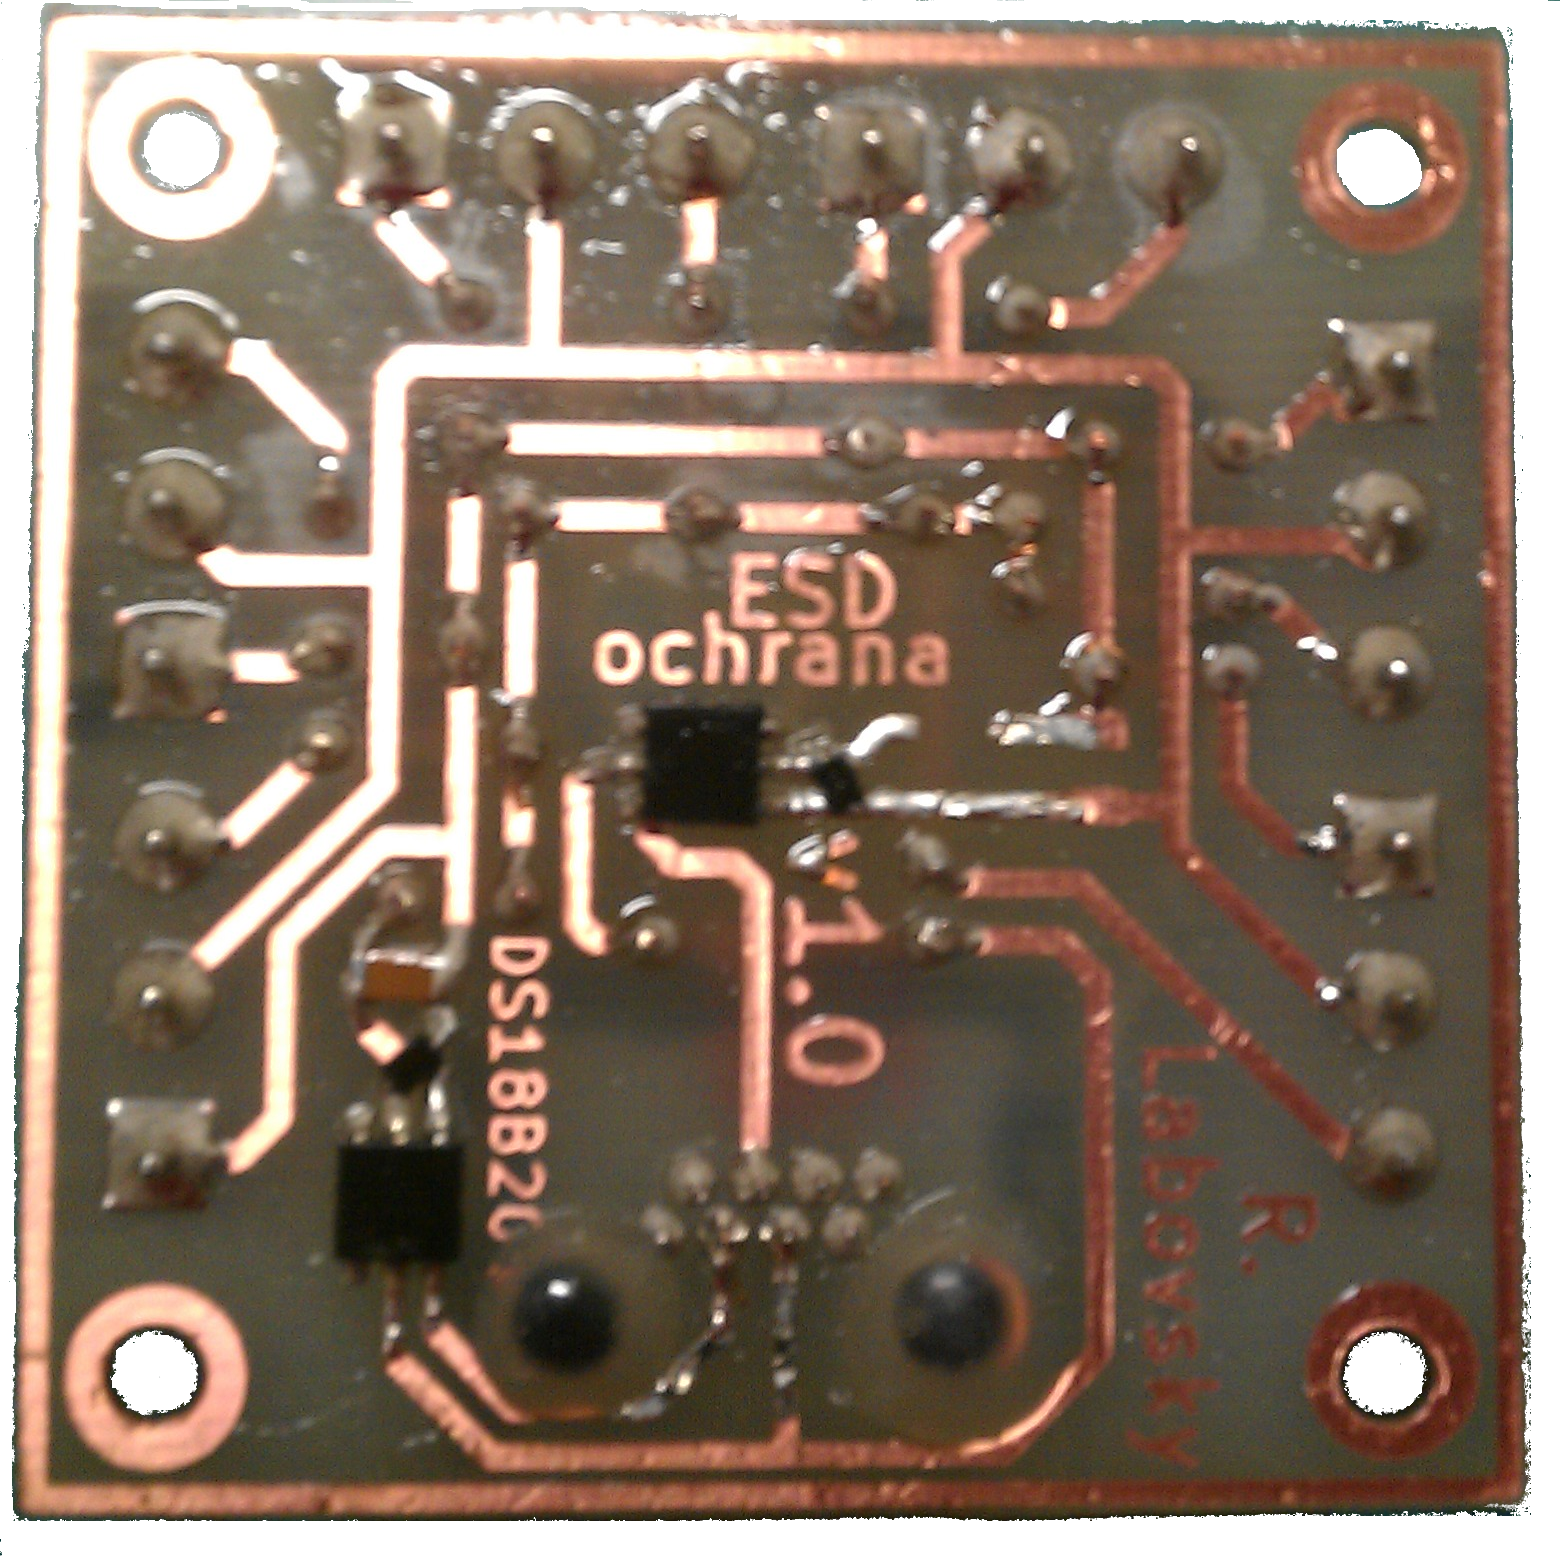
\includegraphics[width=\textwidth]{images/zasobnik-otopne-vody/dps-1-wire-sbernice-u-zasobniku-otopne-vody.png}
    \caption{Realizovaná DPS pro teplotní senzory 1-Wire sběrnice u zásobníku otopné vody.}
    \label{fig:dps-1-wire-sbernice-u-zasobniku-otopne-vody}
\end{subfigure}%
\begin{subfigure}{.5\textwidth}
   	\centering
    \includegraphics[width=0.95\textwidth]{images/zasobnik-otopne-vody/instalacni-krabice-cidla-u-zasobniku-otopne-vody.png}
    \caption{Horní část DPS umístěná do instalační krabice.}
    \label{fig:instalacni-krabice-cidla-u-zasobniku-otopne-vody}
\end{subfigure}%
\caption{Sdružení 1-Wire sběrnice u zásobníku otopné vody}
\end{figure}

%\begin{figure}[H]
%    \centering
%    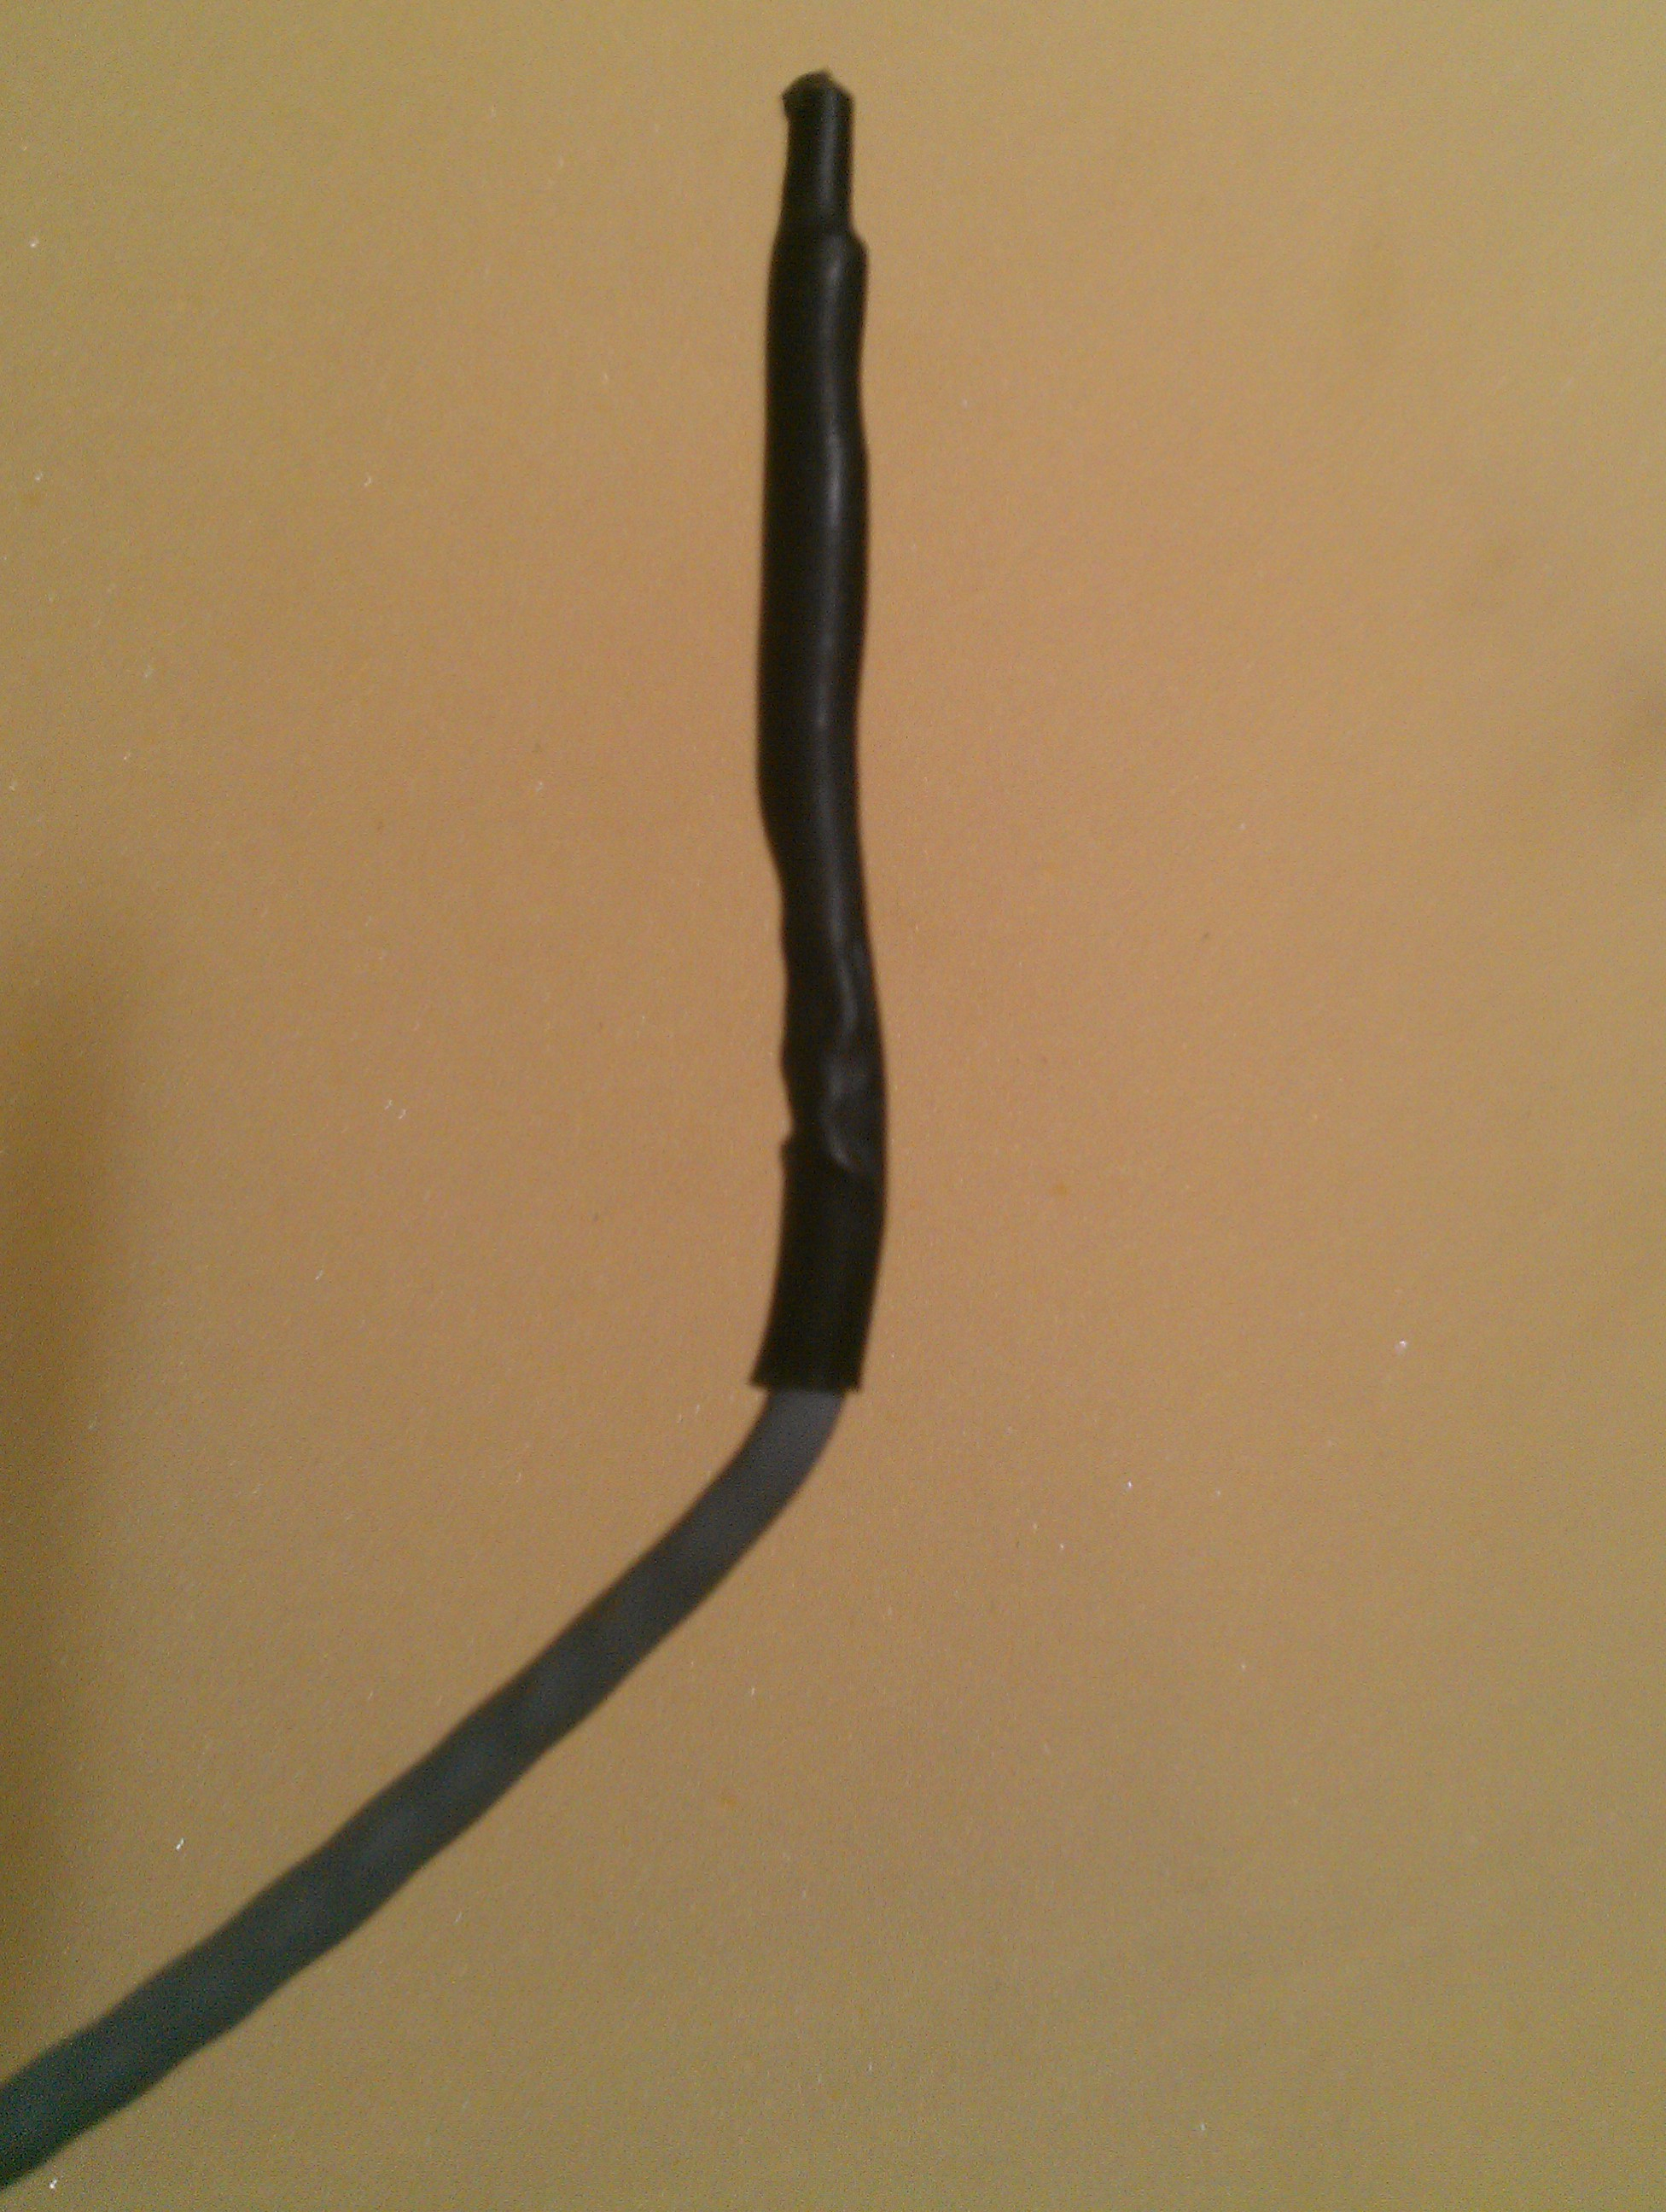
\includegraphics[width=0.4\textwidth]{images/zasobnik-otopne-vody/ds18b20-ochrana.png}
%    \caption{Teplotní senzor DS18B20 v~ochranném pouzdře.}
%    \label{fig:ds18b20-ochrana}
%\end{figure}

\begin{figure}[H]
    \centering
    \includegraphics[width=0.85\textwidth]{images/zasobnik-otopne-vody/zasobnik-otopné-vody.png}
    \caption[Zásobník otopné vody.]{Zásobník otopné vody. Červené kroužky označují místa teplotních senzorů.}
    \label{fig:zasobnik-otopné-vody}
\end{figure}

\section{I$^2$C sběrnice}
\label{sec:i2c-sbernice}

\begin{figure}[H]
   \centering
    \def\svgwidth{0.3\columnwidth}
   \input{images/svg/otopna-soustava/vyrez-i2c-sbernice.pdf_tex}
    \caption[Výřez pro modul I$^2$C sběrnice u centrální jednotky.]{Výřez z obrázku \ref{fig:otopna-soustava-a-elektronika-rez-domu} – modul I$^2$C sběrnice u centrální jednotky.}
    \label{fig:vyrez-i2c-sbernice}
\end{figure}

Na obrázku \ref{fig:vyrez-i2c-sbernice} je výřez části z celkového nákresu (obrázek \ref{fig:otopna-soustava-a-elektronika-rez-domu}) pro modul I$^2$C sběrnici u centrální jednotky. Sběrnice I$^2$C je realizovaná pomocí zakoupeného modulu (obrázek \ref{fig:modul-pca9615-i2c-sbernice}) s~obvodem PCA9615 \cite{vyrobce-pca9615} (blokové schéma je v příloze \ref{fig:blokove-schema-pca9615-i2c-sbernice}) do firmy  NXP Semiconductors. Vstupní signál SCL a~SDA je veden přímo z~centrální jednotky na vstupu obvodu PCA9615, napájení je s 3,3 V logikou. Výstup z PCA9615 je pomocí diferenciální veden. Napájení na této straně je 5 V. Sběrnice je realizovaná pomocí UTP kategorie 5e, výstup z~modulu je realizován pomocí konektoru RJ45. Vzhledem k použití UTP kabelu a diferenciálnímu přenosu je možné dosáhnout velké vzdálenosti sběrnice. Nejdelší bod dosahuje přibližně 30 m, je tedy možné použít I$^2$C sběrnici na vzdálenost, pro kterou není standartě dělána. Použitá frekvence je 100~kHz. Jedná se tedy o plnohodnotnou I$^2$C sběrnici. Důvodem pro zvolení této varianty bylo na základě výběru displeje s I$^2$C sběrnicí (jednoduché a~levné řešení), dále jedná se o klasické zapojení displeje jako by se nalézal v~krátké vzdálenosti od centrální jednotky a není tak nutný převod jako při využít např. RS485 na \acrshort{uart} (\textit{\acrlong{uart}}) a~následně na I$^2$C sběrnici, v neposlední řadě komunikace je definována podle protokolu I$^2$C.  Jeden modul se nalézá na straně centrální jednotky a pak na straně krbů. Napájení 5 V je realizováno pomocí samostatných kabelů, není tedy součástí UTP kabelu. Z důvodu omezení kabeláže je sběrnice realizována v jednom UTP kabelu s 1-Wire sběrnicí, tedy přesněji jsou využity volné vodiče 1,2 pro SCL a~7,~8 pro SDA. Zařízení lze zapojovat jak na straně před PCA9615, tak i~na diferenciální straně, je však výhodné připojené uzly udržet co v~nejkratší vzdálenosti kvůli degradování signálu. Blokové schéma je na obrázku \ref{fig:blokove-schema-pca9615-i2c-sbernice} včetně napojení uzlů. Schéma zapojení modulu v příloze \ref{app:schemata-ostatni}, upraveno z \cite{pca9615-schema-zapojeni}.


Výhodou PCA9615 je automatický výběr směru komunikace, není potřeba externí ovládání. Komunikace je možná až do rychlosti 1 MHz (přibližně pro 3 m), se zvýšenou délkou je však nutné rychlost snížit. Komunikace využívá standardní protokol I$^2$C. Koncová zařízení je možné napájet z různých zdrojů. V neposlední řadě se jedná o jednoduché řešení bez nutných další zařízení na straně Slave, stačí pouze zapojit koncové zařízení s~podporou I$^2$C. Na obrázku \ref{fig:modul-pca9615-transily} jsou pro větší ochranu modulu přidány obousměrné transil diody (SM6T6V8CAY \cite{sm6t6v8cay}) připájené na vstupní piny konektoru RJ45 (obvod sám o sobě poskytuje vstupní ochranu pro ESD). Pro rozbočení I$^2$C sběrnice do jednotlivých pater slouží DPS s konektory RJ45 (schéma viz příloha \ref{app:schemata-ostatni}, obrázky viz příloha \ref{app:rozbocovac-i2c}).

\begin{figure}[H]
\centering
\begin{subfigure}{.5\textwidth}
    \centering
    \includegraphics[width=0.53\textwidth]{images/krb/modul-pca9615-i2c-sbernice.png}
    \caption{Vrchní strana.}
    \label{fig:modul-pca9615-i2c-sbernice}
\end{subfigure}%
\begin{subfigure}{.5\textwidth}
    \centering
    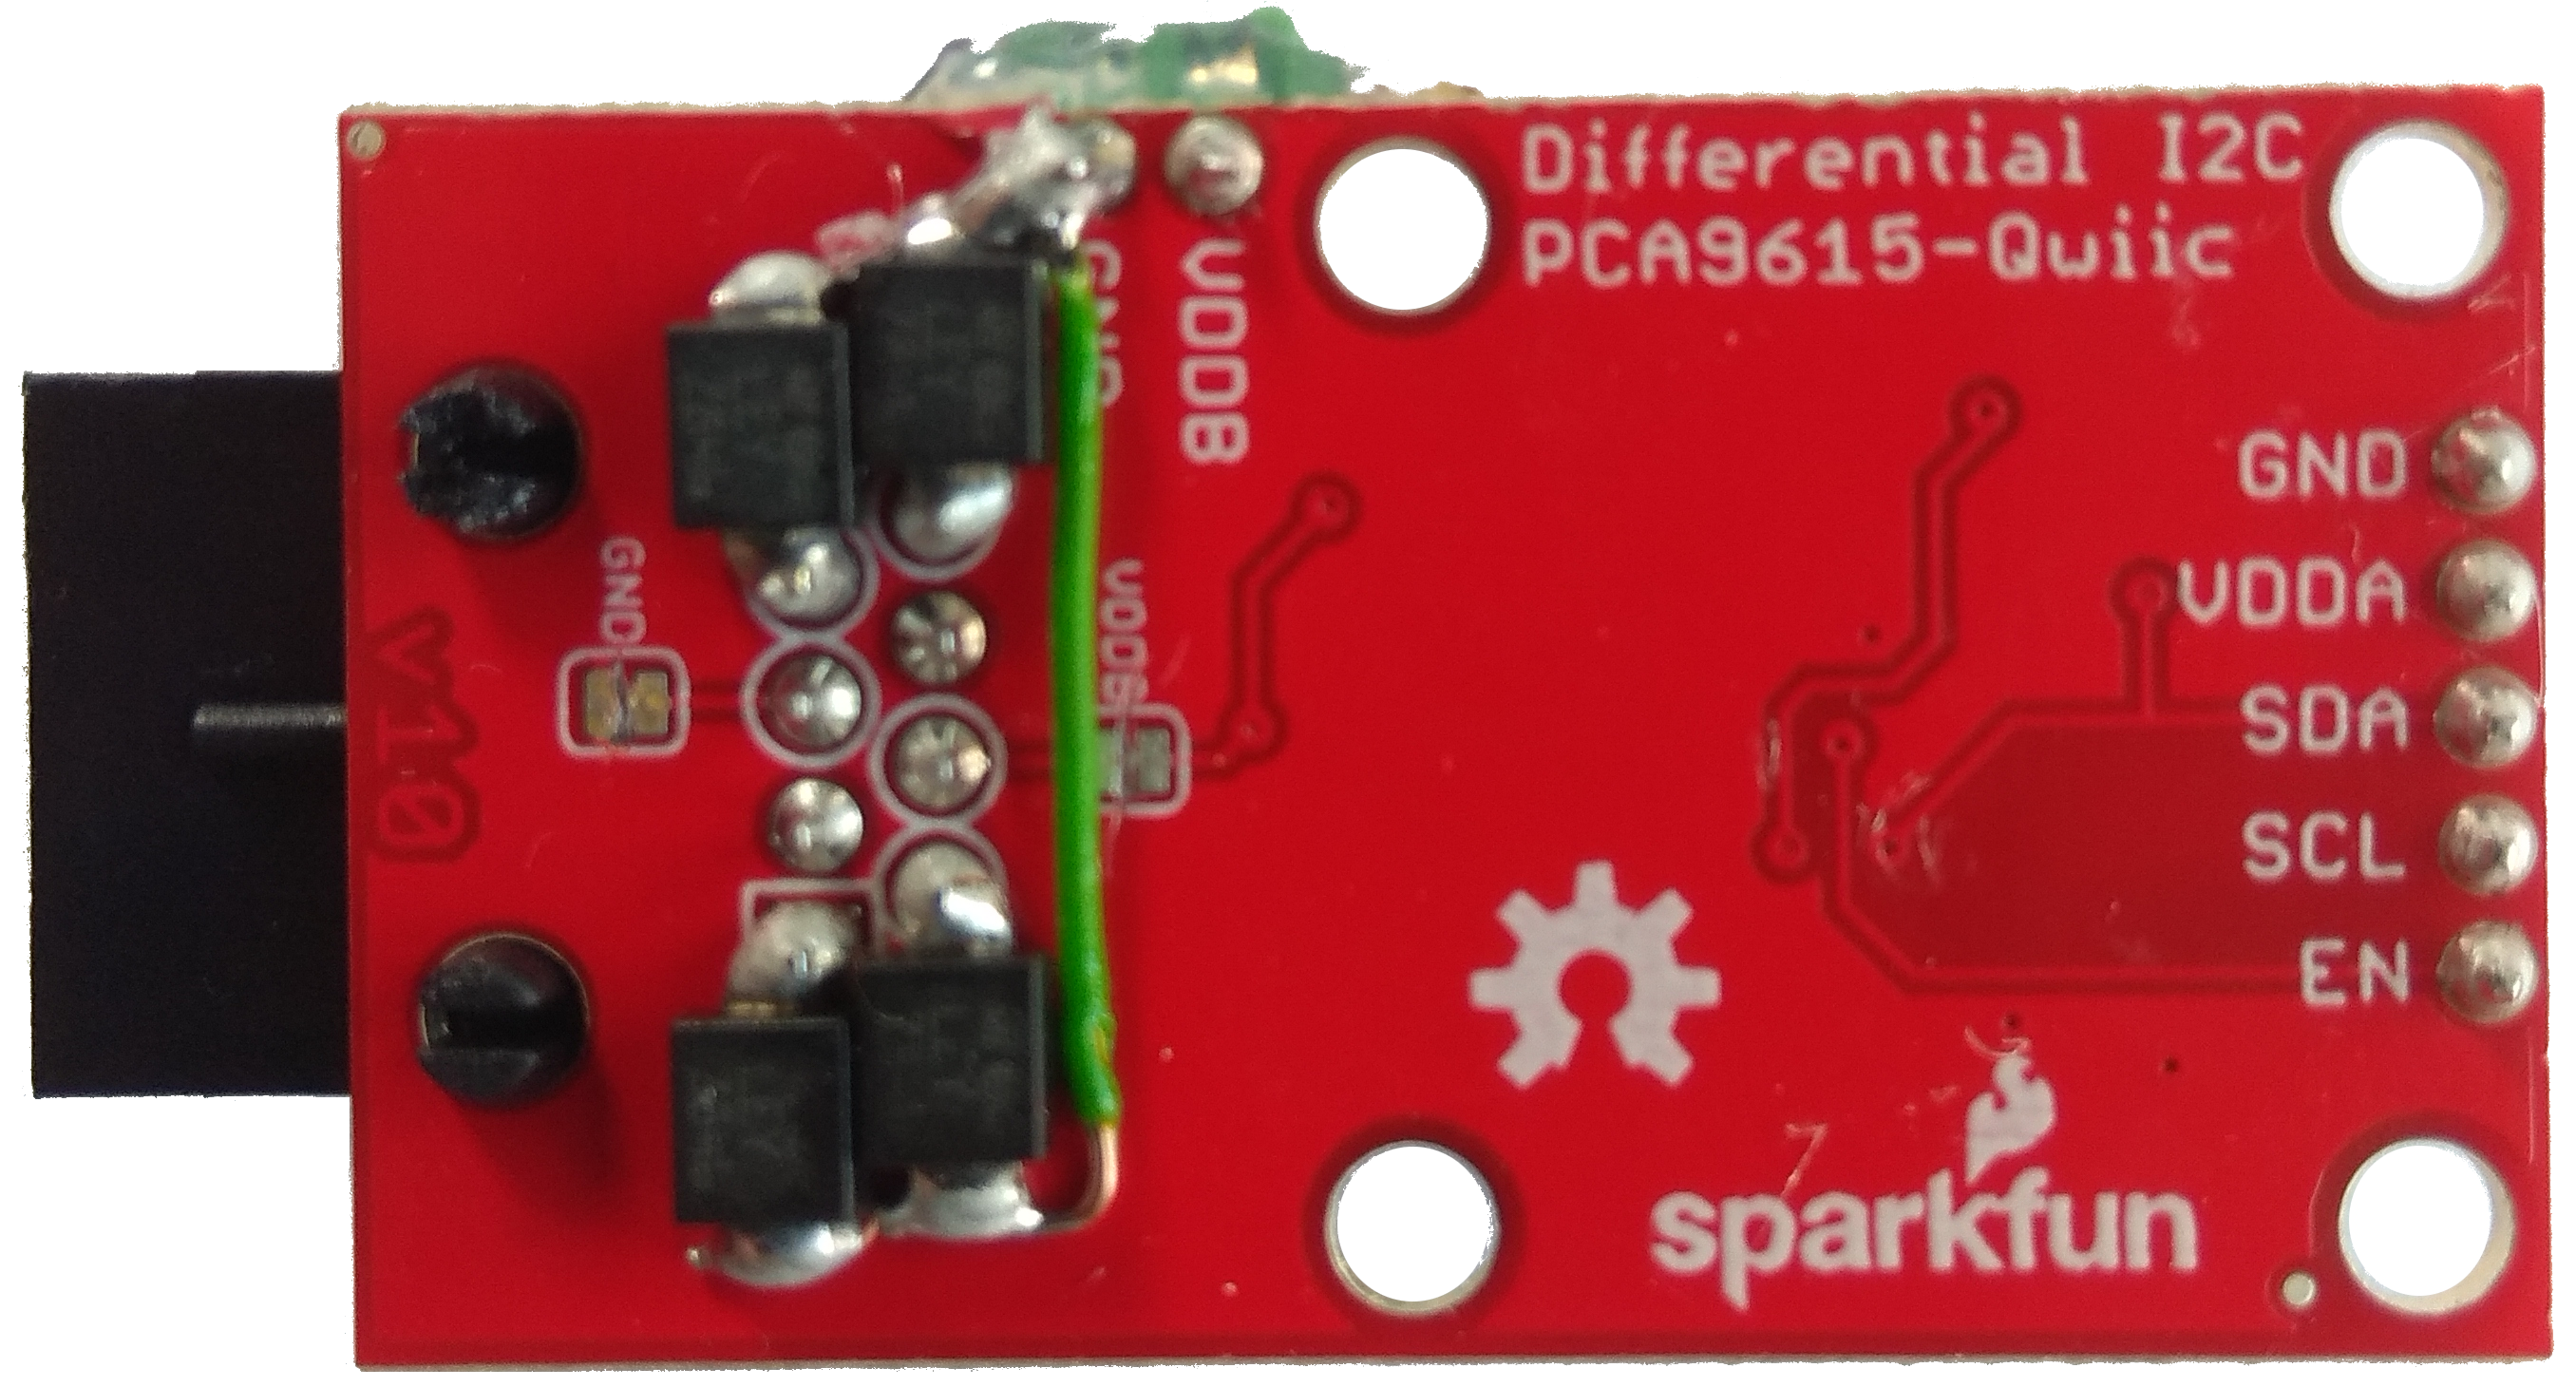
\includegraphics[width=0.6\textwidth]{images/krb/modul-pca9615-transily.png}
    \caption{Spodní strana s ochrannými transily.}
    \label{fig:modul-pca9615-transily}
\end{subfigure}
\caption{Modul s obvodem PCA9615.}
\label{fig:modul-pca9615}
\end{figure}

\section{Připojení 1-Wire sběrnice a chodbových termostatů k centrální jednotce}

\begin{figure}[H]
    \centering
    \def\svgwidth{0.3\columnwidth}
    \input{images/svg/otopna-soustava/vyrez-vstupy-vystupy-rpi.pdf_tex}
    \caption[Výřez pro umístění 1-Wire sběrnici a chodbových termostatů připojených k~centrální jednotce.]{Výřez z obrázku \ref{fig:otopna-soustava-a-elektronika-rez-domu} – umístění 1-Wire sběrnici a chodbových termostatů připojených k~centrální jednotce.}
    \label{fig:vyrez-vstupy-vystupy-rpi}
\end{figure}

\label{sec:dps-se-vstupy-vystupy-pro-raspberry-pi}

Na obrázku \ref{fig:vyrez-vstupy-vystupy-rpi} je výřez části z celkového nákresu (obrázek \ref{fig:otopna-soustava-a-elektronika-rez-domu}) pro umístění 1-Wire sběrnice a~chodbových termostatů.


\subsubsection{Datová část 1-Wire sběrnici}
\label{sec:datova-cast-1-wire-sbernice}
Pro zmíněnou 1-Wire sběrnici jsou realizované ESD ochrany spočívající použití Zenerovy diody a~5~$\Omega$ rezistorů, všechny součástky jsou zaintegrované v~jednom pouzdře TSOC, integrovaný obvod je od výrobce Maxim s označením DS9503 \cite{ds9503}. Integrovaná Zenerova dioda má nízkou kapacitu desítky pF, tím pádem nepřispívá k nadměrnému kapacitnímu zatěžování sběrnice. Omezovací rezistory slouží k omezení proudu při přepěťovém napěťovém impulzu pro ochranu Zenerovy diody (když je otevřena) před nadměrným proudem během ESD události, při běžné komunikace jsou zanedbatelné. Upínací napětí Zenerovy diody je 5,5 V při 0,9 A (průrazné napětí je přibližně 11~V) během ESD události. Dále je zde zařazena \acrshort{tvs} (\textit{\acrlong{tvs}}) dioda (ESD9L5.0ST5G \cite{esd9l5-0st5g}) s upínacím napětím maximálně 9,8 V při 1 A, slouží jako sekundární ochrana, pokud by selhala část s DS9503. 

Další možností je použití galvanického oddělení především pomocí optočlenu. Zde však nastává problém s obousměrnou poloduplexní komunikací, je potřeba zajistit komunikaci oběma směry. Optočleny vkládají zpoždění, které by podle specifikace 1-Wire sběrnice nemělo přesáhnout 1~µs. Dále je potřeba oddělený převodník napětí či samotný zdroj pro napájení oddělených částí optočlenu a~další potřebné externí součástky. V neposlední řadě je nutné, alespoň podle výrobce Maxim,  použít převodník UART na 1-Wire či I$^2$C na 1-Wire sběrnici. Řešení pomocí galvanického oddělení ve výsledku zesložiťuje řešení a též prodražuje. Vzhledem k domácímu nasazení byla zvolena varianta podle obrázku~\ref{fig:ochrany-1-wire}.

Napěťová tolerance pro piny Raspberry Pi je 3,3 V. Proto je použit obousměrný převodník napěťových úrovní z 3,3 V na 5~V a opačně, realizovaný pomocí MOSFET tranzistoru (BSS138P \cite{bss138p}), pull-up rezistorů.

Na obrázku \ref{fig:ochrany-1-wire} jsou vidět dvě větve pro 1-Wire sběrnici, je to z důvodu dvou typů zařízení, teplotních čidel DS18B20 a zesilovače/převodníku MAX31850K \cite{max31850k} s termočlánkem , které mají různé časování, sběrnice je popsána v \ref{sec:1-wire-sbernice}. Sběrnici, lze sdružit do jedné pomocí propojky P6.

\begin{figure}[H]
    \centering
    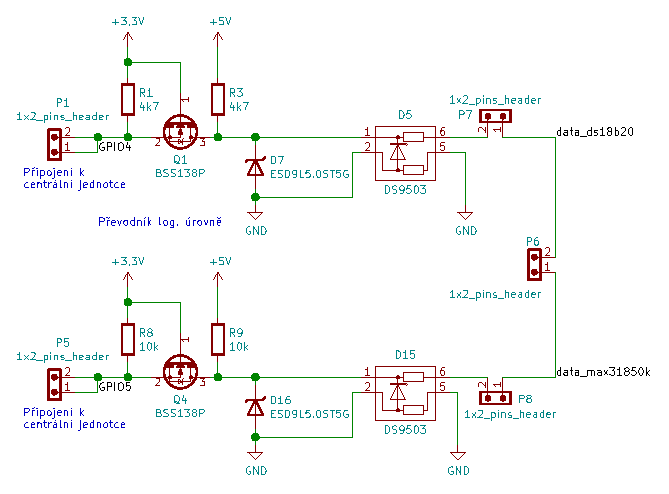
\includegraphics[width=0.9\textwidth]{images/svg/kicad/ochrany-1-wire.eps}
    \caption[ESD ochrany pro 1-Wire sběrnici s~převodníkem log. úrovní.]{ESD ochrany pro 1-Wire sběrnici s převodním log. úrovní. Kolíková lišta P1, P5 je připojena na Raspberry Pi.}
    \label{fig:ochrany-1-wire}
\end{figure}


\subsubsection{Napájení 1-Wire sběrnice}
\label{sec:napajeni-1-wire-sbernice}
Pro ochranu napájení 1-Wire sběrnice (5 V) jsou veškeré koncové teplotní senzory napájené přes elektronickou pojistku od Texas Instrumenst s označením TPS2600 \cite{tps26600}, schéma zapojení na obrázku \ref{fig:ochrana-napajeni-1-wire}. Obvod zajišťuje ochranu pro vstupní napětí, hlídá maximální hodnotu vstupního napětí do nastavené meze 5,25 V (maximální hranice je 60 V), minimální vstupní napětí do nastavené meze 4,75 V (minimální hranice je -60 V). Vstupní omezení napětí je pomocí rezistorů R5, R10, R11 a~R12. Omezovací proud je nastaven na přibližně 73~mA (hodnotu lze změnit přes potenciometr R17), při jeho překročení dojde k~odpojení výstupu po dobu, dokud nedojde k~odstranění závady. Kondenzátor C2 nastavuje rychlost náběhu výstupního napětí. Pro indikaci chyb napájení je červená LED.

\begin{figure}[H]
    \centering
    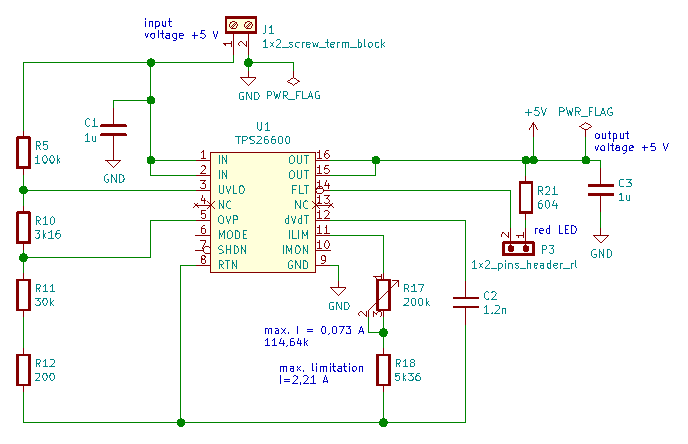
\includegraphics[width=\textwidth]{images/svg/kicad/ochrana-napajeni-1-wire.eps}
    \caption{Obvod TPS26600 pro ochranu napájení 1-Wire sběrnice.}
    \label{fig:ochrana-napajeni-1-wire}
\end{figure}

\subsubsection{Ochrana pro chodbové nástěnné termostaty}
Obdobně jako v části \ref{sec:datova-cast-1-wire-sbernice} (datová část 1-Wire sběrnice) je stejná ochrana pro snímání logické úrovně z~chodbových termostatů. Při sepnutí termostatu na daném patře je detekována log. 0 (požadavek na vytápění) v opačném případě je zde log. 1 (zastavení vytápění). Chodbové  termostaty jsou popsány v sekci \ref{sec:digitalni-chodbove-termostaty}.

\subsubsection{Ochrana napájení 3,3 V}
Přímo z Raspberry Pi je využito napětí 3,3 V pro převodník napětí, popsaný v~části \ref{sec:datova-cast-1-wire-sbernice} (datová část 1-Wire sběrnice). Zde je použita vratná pojistka polymerový \acrshort{ptc} (\textit{\acrlong{ptc}}) (RXEF005 \cite{rxef005}) se spínacím proudem 100 mA, pro omezení proudu v~případě poruchy, dále je zde transilová dioda (SM2T3V3A \cite{sm2t3v3a}) pro ochranu při přepětí (s~upínacím napětím max. 6,5~V (při 25 A, 10/1000~µs), průrazné napětí 3,6~V). Na obrázku \ref{fig:ochrana-napajeni-3_3-v} je zobrazena popsaná ochrana.

\begin{figure}[H]
    \centering
    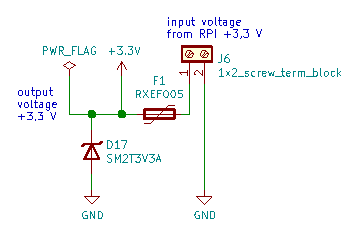
\includegraphics[width=0.6\textwidth]{images/svg/kicad/ochrana-napajeni-3_3-v.eps}
    \caption{Ochrana pro výstupní napětí 3,3 V z~Raspberry Pi.}
    \label{fig:ochrana-napajeni-3_3-v}
\end{figure}


\subsubsection{Realizovaná DPS ochran pro centrální jednotku Raspberry Pi}
Na obrázku \ref{fig:dps-pro-ochranu-vstupu-vystupu-pro-raspberry-pi} je realizovaná DPS vstupů/výstupů pro centrální jednotku Raspberry Pi. Ze samotné DPS je sběrnice vyvedena pomocí konektorů RJ45, čtyři konektory pro teplotní senzory DS18B20 a čtyři pro termočlánky s MAX31850K. Celkové schéma zapojení je v příloze \ref{app:schemata-ostatni}.

\begin{figure}[H]
\centering
\begin{subfigure}{.5\textwidth}
    \centering
    \includegraphics[width=0.6\textwidth]{images/vstupy-vystupu-rpi/dps-rpi-1-wire-termostaty-ochrany-spodek.png}
    \caption{Spodní část.}
    \label{fig:dps-rpi-1-wire-termostaty-ochrany-spodek}
\end{subfigure}%
\begin{subfigure}{.5\textwidth}
    \centering
    \includegraphics[width=0.7\textwidth]{images/vstupy-vystupu-rpi/dps-rpi-1-wire-termostaty-ochrany-vrsek.png}
    \caption{Vrchní část.}
    \label{fig:dps-rpi-1-wire-termostaty-ochrany-vrsek}
\end{subfigure}
\caption{DPS pro 1-Wire sběrnici a chodbové termostaty připojené k centrální jednotce.}
\label{fig:dps-pro-ochranu-vstupu-vystupu-pro-raspberry-pi}
\end{figure}

\section{Signalizace stavů u krbů}
\begin{figure}[H]
   \centering
    \def\svgwidth{0.3\columnwidth}
    \input{images/svg/otopna-soustava/vyrez-krb-signalizace.pdf_tex}
    \caption[Výřez pro umístění signalizace stavů u krbu.]{Výřez z obrázku \ref{fig:otopna-soustava-a-elektronika-rez-domu} – umístění signalizace stavů u krbu.}
    \label{fig:vyrez-krb-signalizace}
\end{figure}

Na obrázku \ref{fig:vyrez-krb-signalizace} je výřez části z celkového nákresu (obrázek \ref{fig:otopna-soustava-a-elektronika-rez-domu}) pro signalizaci stavů u krbu. Navržená DPS se skládá z části elektronické pojistky TPS2600, zapojení je obdobné jako v \ref{sec:napajeni-1-wire-sbernice} (napájení 1-Wire sběrnice), navíc je na vstupu připojena transilová dioda (ESD9L5.0ST5G). Napěťové meze jsou nastaveny stejně, tedy minimální napětí je 4,75 V, maximální 5,25 V, proud je omezen na maximální hodnotu 100 mA. Dále je zde přivedena 1-Wire sběrnice přes konektor RJ45 s~obdobnými ochranami jako v \ref{sec:datova-cast-1-wire-sbernice} (datová část 1-Wire sběrnice) pro připojení MAX31850K přes svorkovnici. V neposlední řadě jsou zde vstupy pro ovládání třech LED pro signalizaci (obrázek \ref{fig:led-indikace}) naakumulovaného zásobníku otopné vody, modrá LED signalizuje stav horní části zásobníku, oranžová LED je pro střední část, červená je pro signalizaci spodní části. Vstupní část je chráněná přes DS9503 a transilovou diodou (ESD9L5.0ST5G). Sepnutí LED je přes tranzistor (BSS138P). Obdobně jsou řešeny oranžová a modrá LED. Celkové schéma zapojení je v~příloze \ref{app:schemata-ostatni}.

\begin{figure}[H]
    \centering
    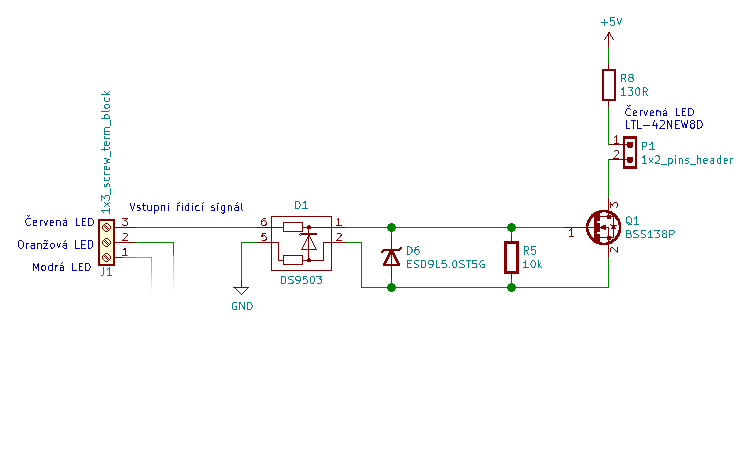
\includegraphics[width=\textwidth]{images/svg/kicad/led-indikace.eps}
    \caption{Zapojení pro ovládání signalizační červené LED.}
    \label{fig:led-indikace}
\end{figure}




\subsubsection{Měření teploty pomocí termočlánku a převodníku MAX31850K}
Teplotní senzory připojené na kouřovody krbů jsou realizované pomocí termočlánku z \ref{sec:teplotni-senzory-pro-krby}. Termočlánek je připojený k zakoupenému modulu (obrázek~\ref{fig:modul-max31850k-1-wire-prevodnik-termoclanku}), hodnota napětí z termočlánku je převedena do digitální podoby včetně teplotní kompenzace studeného konce a~tato hodnota je poslána po 1-Wire sběrnici. Je možné připojit termočlánek typu K. Převodník umožňuje měřit teplotu s~převodem pomocí AD převodníku až na 14 bitů. Rozlišení teploty činí 0,25~°C. Při teplotách -200 °C až 700 °C činí přesnost měřené teploty ±2~°C. Obvod disponuje detekcí zkratu (na GND nebo napájení) na vstupu pro termočlánek. Dále je zde detekce odpojeného termočlánku. Schéma zapojení modulu je v příloze \ref{app:schemata-ostatni}, upraveno z \cite{prevodnik-max31850k}.

%\begin{figure}[H]
%    \centering
%    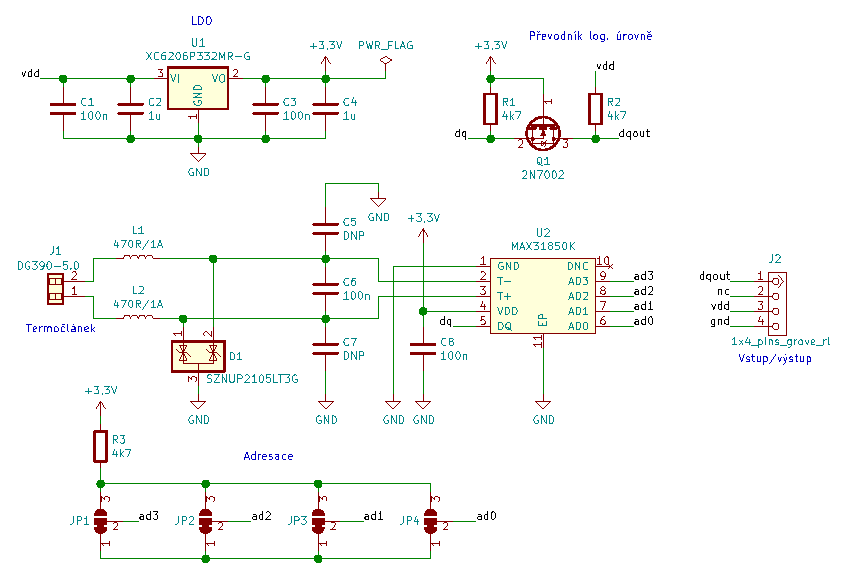
\includegraphics[width=\textwidth]{images/svg/kicad/zapojeni-max31850k-1-wire-prevodnik-termoclanku.eps}
%    \caption[Zapojení MAX31850K v modulu.]{Zapojení MAX31850K v modulu. Upraveno z \cite{prevodnik-max31850k}.}
%    \label{fig:zapojeni-max31850k-1-wire-prevodnik-termoclanku}
%\end{figure}

\begin{figure}[H]
    \centering
    \includegraphics[width=0.4\textwidth]{images/krb/modul-max31850k-1-wire-prevodnik-termoclanku.png}
    \caption[Modul s obvodem MAX31850K.]{Modul s obvodem MAX31850K \cite{prevodnik-max31850k}.}
    \label{fig:modul-max31850k-1-wire-prevodnik-termoclanku}
\end{figure}

\subsubsection{LCD displej}
Pro zobrazování teplot ze střední a spodní části zásobníku otopné vody byl zvolen 16 znakový a 2 řádkový LCD displej s modrým podsvícením a~bílými písmeny (obrázek \ref{fig:lcd-displej}). Pro obsluhu displeje slouží řadič HD44780. K~řadiči je připojen I$^2$C expandér PCF8574 s osmi výstupy, které jsou připojeny na datovou sběrnici pro ovládání respektive zobrazování znaků na displeji. Displej je zapojen za modulem popsaným v části \ref{sec:i2c-sbernice} (I$^2$C sběrnice). Každý displej, respektive expandér PCF8574 umožňuje nastavit pomocí propojek A0, A1, A2 unikátní adresu zařízení na sběrnici.

\begin{figure}[H]
\centering
\begin{subfigure}{.5\textwidth}
  \centering
  \includegraphics[width=0.91\linewidth]{images/krb/predni-cast-lcd-displeje.png}
  \caption{Přední část displeje.}
  \label{fig:predni-cast-lcd-displeje}
\end{subfigure}%
\begin{subfigure}{.5\textwidth}
  \centering
  \includegraphics[width=0.9\linewidth]{images/krb/zadni-cast-lcd-displeje-s-expanderem-pcf8574.png}
  \caption{Zadní část displeje s I$^2$C expandérem PCF8574.}
  \label{fig:zadni-cast-lcd-displeje-s-expanderem-pcf857}
\end{subfigure}
\caption[LCD displej pro zobrazování teplot ze zásobníku otopné vody.]{LCD displej pro zobrazování teplot ze zásobníku otopné vody \cite{lcd-displej}.}
\label{fig:lcd-displej}
\end{figure}

\subsubsection{Realizovaná DPS signalizace u krbů}
Výše popsané části jsou realizované na DPS (obrázek \ref{fig:dps-led-ochrany-u-krbu-spodek}, \ref{fig:dps-led-ochrany-u-krbu-vrsek}, \ref{fig:dps-led-ochrany-u-krbu-kabely}). Deska byla vlastnoručně navržena, vyrobena a osazena. Je aplikován ochranný lak. Celkové schéma zapojení je v příloze \ref{app:schemata-ostatni}.

\begin{figure}[H]
    \centering
    \includegraphics[width=0.8\textwidth]{images/krb/dps-led-ochrany-u-krbu-spodek.png}
    \caption{Spodní část DPS pro signalizaci u krbu.}
    \label{fig:dps-led-ochrany-u-krbu-spodek}
\end{figure}

\begin{figure}[H]
    \centering
    \includegraphics[width=0.8\textwidth]{images/krb/dps-led-ochrany-u-krbu-vrsek.png}
    \caption{Horní část DPS pro signalizaci u krbu.}
    \label{fig:dps-led-ochrany-u-krbu-vrsek}
\end{figure}

\begin{figure}[H]
    \centering
    \includegraphics[width=0.8\textwidth]{images/krb/dps-led-ochrany-u-krbu-kabely.png}
    \caption{DPS včetně signalizačních LED.}
    \label{fig:dps-led-ochrany-u-krbu-kabely}
\end{figure}

\subsubsection{Instalační krabice}
Všechna elektronika je umístěna do ochranné instalační krabice (obrázek \ref{fig:instalacni-krabice-vnitrek-krb}). Do krabice vstupují dva vodiče pro napětí 5 V a zem, tři kabely pro ovládání signalizačních LED, UTP kabel se sběrnicí 1-Wire pro teplotní senzor (termočlánek) a I$^2$C sběrnicí. Na obrázku \ref{fig:zadni-cast-krytu-vika-instalacni-krabice-krb} je zobrazena zadní část víka instalační krabice s uchycením signalizačních LED a LCD displeje. Na obrázku \ref{fig:predni-cast-krytu-vika-instalacni-krabice-krb} je přední část víka instalační krabice. Takto zkompletovaná instalační krabice je umístěna u krbu ve sklepě, v přízemí a v patře.

%\begin{figure}[H]
%    \centering
%    \includegraphics[width=0.6\textwidth]{images/krb/instalacni-krabice-vnitrek-krb.png}
%    \caption{Instalační krabice s jednotlivými moduly.}
%    \label{fig:instalacni-krabice-vnitrek-krb}
%\end{figure}

%\begin{figure}[H]
%    \centering
%    \includegraphics[width=0.6\textwidth]{images/krb/zadni-cast-krytu-vika-instalacni-krabice-krb.png}
%    \caption{Zadní část instalační krabice.}
%    \label{fig:zadni-cast-krytu-vika-instalacni-krabice-krb}
%\end{figure}



\begin{figure}[H]
\centering
\begin{subfigure}{.5\textwidth}
  \centering
  \includegraphics[width=0.835\textwidth]{images/krb/instalacni-krabice-vnitrek-krb.png}
  \caption{Instalační krabice s jednotlivými moduly.}
  \label{fig:instalacni-krabice-vnitrek-krb}
\end{subfigure}%
\begin{subfigure}{.5\textwidth}
  \centering
  \includegraphics[width=\textwidth]{images/krb/zadni-cast-krytu-vika-instalacni-krabice-krb.png}
  \caption{Zadní část instalační krabice.}
  \label{fig:zadni-cast-krytu-vika-instalacni-krabice-krb}
\end{subfigure}
\caption{Instalační krabice pro signalizaci stavů.}
\label{fig:instalacni-krabice}
\end{figure}



\begin{figure}[H]
    \centering
    \includegraphics[width=0.55\textwidth]{images/krb/predni-cast-krytu-vika-instalacni-krabice-krb.png}
    \caption[Víko instalační krabice.]{Víko instalační krabice. Osazený LCD displej, signalizačních LED (zleva modrá, oranžová a červená) a LED pro aktivování elektronické pojistky (červená LED vlevo od displeje).}
    \label{fig:predni-cast-krytu-vika-instalacni-krabice-krb}
\end{figure}




\section{Zónový regulátor}
Zónový regulátor se skládá s modulu PCA9615 (viz část \label{ses:i2c-sbernice} (I$^2$C)) pro realizaci I$^2$C sběrnice pomocí diferenciálních párů. Na modul je následně napojen zakoupený modul s obvodem PCA9685 od firmy NXP Semiconductors. Výstupy z modulu jsou napojeny na DPS, která zapíná/vypíná (respektive PWM regulace) jednotlivé termoelektrické pohony (celkově 12 pohonů, každý je řízen samostatně), čímž dochází k regulaci otopné vody do otopných okruhů. Zonové regulátory jsou umístěny u rozdělovače otopných okruhů v přízemí a~patře domu, celkově se jedná o dvě vyrobená zařízení.

\subsubsection{PCA9685}
Modul s obvodem PCA9685 umožňuje pomocí I$^2$C sběrnice ovládat 16 výstupů se stejnou individuální hodnotou PWM (se střídou 0 \% až 100 \%), frekvence je programovatelná od 24 Hz do 1\,526 Hz. Každý kanál navíc může dodat 10~mA jako source, případně 25 mA jako sink (což je 160 mA respektive 400~mA celkově).

\subsubsection{DPS pro ovládání termoelektrických pohonů}
Termoelektrické pohony jsou ovládány na základě hodnoty PWM z modulu PCA9685 (viz předchozí bod), každý výstupu ovládá jednotlivý pohon. Vzhledem k tomu, že termoelektrické pohony jsou na stejnosměrné napětí 24 V, je nutné využít napěťový převodník z 5 V na 24 V. K tomu slouží tranzistor MOSFET (DMN3023L-7). V závislosti na hodnotě PWM na jeho vstupu (gate) je otevírán/zavírán a dochází tak k regulaci napětí/proudu v~termoelektrickém pohonu, který je zapojen jako zátěž (přes drain). Paralelně k~tranzistoru se nachází přepínač, který slouží v případě poruchy k manuálnímu zapnutí/vypnutí pohonu. Přepínač má jmenovitý proud 0,5~A, což je dostatečné pro termoelektrický pohon, kterým při zapnutí teče maximální proud 250 mA (následně dochází ke snižování a saturaci proudu). Každý kanál obsahuje zelenou LED pro signalizaci, zda dochází k ovládání. Jak již bylo řečeno pohony jsou napájeny pomocí 24 V, jsou vytvořené dvě napájecí větve s obvodem TPC26600 (popsaný v části \ref{sec:napajeni-1-wire-sbernice}), rozdíl spočívá ve vstupním napájení, které činí 24 V. Jsou tedy rozdílné i~maximální a~minimální povolené meze, které činí max. 24,25 V a min. 10~V. Dále každá větev má nastavený maximální proud 1,5 A (každý pohon má maximální hodnotu proudu při zapnutí 250 mA pro celkově 6 pohonů na větev). Vzhledem k jednoduchosti obvodu TPS26600 a k jeho vlastnostem (především pro automatickou detekci odstranění závady, bez nutnosti restartu zařízení) bylo raději zvoleno zapojení se dvěma větvemi (maximální proud pro TPS26600 činí 2,21 A) než využití jiného integrovaného obvodu pro sloučení do jedné větve. Na obrázku \ref{fig:zonovy-regulator-mosfet-pwm-1-kanal} je zapojení jednoho kanálu pro ovládání termoelektrického pohonu.  Na obrázku \ref{fig:dps-zonovy-regulator-spodni-strana} spodní strana realizované DPS a na obrázku \ref{fig:zonovy-regulator-vrchni-strana} je vrchní strana, včetně osazeného modulu s obvodem PCA9615. Na obrázku \ref{fig:zonovy-regulator-spodni-strana} je spodní část panelu s DPS zonového regulátoru a na obrázku \ref{fig:zonovy-regulator-vrchni-strana} je čelní část panelu.  Celkové schéma zapojení je v příloze \ref{app:schemata-ostatni}. Umístění DPS v samotném rozdělovači pro přízemí je v příloze \ref{app:rozdelovac-podlahoveho-vytapeni}.


\begin{figure}[H]
    \centering
    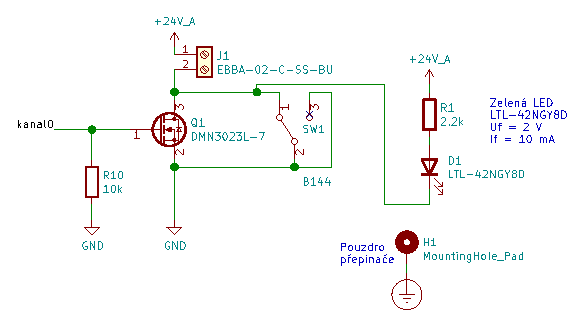
\includegraphics[width=\textwidth]{images/svg/kicad/zonovy-regulator-mosfet-pwm-1-kanal.eps}
    \caption{Zapojení jednoho kanálu pro ovládání termoelektrického pohonu.}
    \label{fig:zonovy-regulator-mosfet-pwm-1-kanal}
\end{figure}

\begin{figure}[H]
    \centering
    \includegraphics[width=0.99\textwidth]{images/zonovy-regulator/dps-zonovy-regulator-spodni-strana.png}
    \caption{DPS zonového regulátoru, spodní strana.}
    \label{fig:dps-zonovy-regulator-spodni-strana}
\end{figure}

\begin{figure}[H]
    \centering
    \includegraphics[width=0.99\textwidth]{images/zonovy-regulator/dps-zonovy-regulator-vrchni-strana.png}
    \caption{DPS zonového regulátoru, vrchní strana.}
    \label{fig:dps-zonovy-regulator-vrchni-strana}
\end{figure}


\begin{figure}[H]
    \centering
    \includegraphics[width=0.95\textwidth]{images/zonovy-regulator/zonovy-regulator-spodni-strana.png}
    \caption{Zadní část panelu zónového regulátoru.}
    \label{fig:zonovy-regulator-spodni-strana}
\end{figure}

\begin{figure}[H]
    \centering
    \includegraphics[width=0.95\textwidth]{images/zonovy-regulator/zonovy-regulator-vrchni-strana.png}
    \caption[Čelní část panelu zónového regulátoru.]{Čelní část panelu zónového regulátoru se signalizačními LED a~manuálním ovládáním pomocí spínačů.}
    \label{fig:zonovy-regulator-vrchni-strana}
\end{figure}



\subsubsection{Termoelektrické pohony Salus T30NC}  
Termoelektrický pohon Salus T30NC slouží k ovládání ventilů pro jednotlivé otopné okruhy. Je napájen stejnosměrným napětí 24 V při maximálním proudovém odběru při zapnutí 250 mA. Provozní příkon jsou 2 W. Rozměr závitu je M30\,×\,1,5. Maximální délka zdvihu pro dřík ventilu činí 4 mm. Síla pohonu je 100 N ($\pm$10 \%). Čas pro otevření je přibližně 2 minuty. Jedná se o~typ \acrshort{nc} (\textit{\acrlong{nc}}), při odpojení napájení je ventily zavřen. Pohon má funkci „First Open“ neboli je možné pomocí zarážky ventil instalovat jako otevřený bez nutnosti napájení (využít v případě, kdy není ještě instalovaná centrální jednotka). Pro každé patro je použito 12 těchto pohonů.

\begin{figure}[H]
    \centering
    \includegraphics[width=0.8\textwidth]{images/termoelektricky-pohon-salus-t30nc-24-v.png}
    \caption[Termoelektrický pohon Salus T30NC na stejnosměrné napětí 24 V.]{Termoelektrický pohon Salus T30NC na stejnosměrné napětí 24~V \cite{termoelektricky-pohon-t30nc}.}
    \label{fig:termoelektricky-pohon-salus-t30nc-24-v}
\end{figure}

\section{Digitální chodbové termostaty}
\label{sec:digitalni-chodbove-termostaty}
\begin{figure}[H]
   \centering
   \def\svgwidth{0.4\columnwidth}
   \input{images/svg/otopna-soustava/vyrez-lokalni-termostaty.pdf_tex}
    \caption[Výřez pro umístění chodbových termostatů.]{Výřez z obrázku \ref{fig:otopna-soustava-a-elektronika-rez-domu} – umístění chodbových termostatů.}
    \label{fig:vyrez-lokalni-termostaty}
\end{figure}

Na obrázku \ref{fig:vyrez-lokalni-termostaty} je výřez části z celkového nákresu (obrázek \ref{fig:otopna-soustava-a-elektronika-rez-domu}) systému znázorňující umístění chodbových termostatů. Pro snímání teplot z jednotlivých pater na chodbách slouží zakoupené digitální termostaty s označením W3230 \cite{digitalni-termostat-w3230}. Termostat disponuje jedním spínací výstupem (v případě potřeby vytápění se výstup sepne, jinak je rozepnut). Je možné nastavit hysterezi, časové zpoždění, kalibraci teploty a rozsah maximálních teplot. Lze také aktivovat signalizaci, která se spustí po dosažení maximální přípustné teploty. Pro napájení je potřeba stejnosměrné napětí 12 V. Pro snímání teploty slouží NTC termistor. Rozsah teplot je -40 °C až 120 °C. Přesnost měření je $\pm$ 0,1 °C. Termostat lze nahradit za jakýkoliv jiný, který disponuje spínacím výstupem.


\begin{figure}[H]
    \centering
    \includegraphics[width=0.5\textwidth]{images/digitalni-termostat-w3230.png}
    \caption[Digitální chodbový termostat W3230.]{Digitální chodbový termostat W3230 \cite{digitalni-termostat-w3230}.}
    \label{fig:digitalni-termostat-w3230}
\end{figure}

\section{Spínací jednotka}
\begin{figure}[H]
   \centering
   \def\svgwidth{0.4\columnwidth}
   \input{images/svg/otopna-soustava/vyrez-spinaci-jednotka.pdf_tex}
    \caption[Umístění spínacích jednotek.]{Výřez z obrázku \ref{fig:otopna-soustava-a-elektronika-rez-domu} – spínací jednotky.}
    \label{fig:vyrez-spinaci-jednotka}
\end{figure}
Na obrázku \ref{fig:vyrez-spinaci-jednotka} je výřez části z celkového nákresu (obrázek \ref{fig:otopna-soustava-a-elektronika-rez-domu}) pro spínací jednotky. Pro spínání čerpadel a signalizačních LED slouží dva zakoupené relé moduly po čtyřech kanálech \cite{rele-modul-informace}. Relé umožňují spínat výkony 250 VAC při max. 10~A a 30 V DC při max. 10~A. Jednotlivé kanály jsou oddělené galvanicky (dále je vyfrézovaná část DPS mezi výkonovou částí a spínací částí), též je možné využít různých zdrojů pro napájení spínací části a napájení relé. Zapojení jednoho kanálu je v příloze \ref{app:schemata-ostatni}. Celý relé modul je na obrázku \ref{fig:ctyr-kanalovy-rele-modul}. Pro spínání síťového napětí je použit jeden relé modul, pro spínání slaboproudého napětí (LED diody, kotel) je použit druhý relé modul.

%\begin{figure}[H]
%    \centering
%    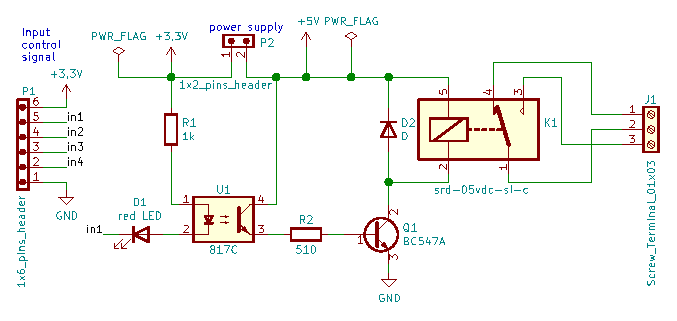
\includegraphics[width=\textwidth]{images/svg/kicad/rele-modul-jeden-kanal.eps}
%    \caption{Zapojení jednoho kanálu relé modulu.}
%    \label{fig:rele-modul-jeden-kanal}
%\end{figure}


\begin{figure}[H]
    \centering
    \includegraphics[width=0.5\textwidth]{images/ctyr-kanalovy-rele-modul.png}
    \caption[Čtyřkanálový relé modul.]{Čtyřkanálový relé modul \cite{ctyr-kanalovy-rele-modul}.}
    \label{fig:ctyr-kanalovy-rele-modul}
\end{figure}

\section{Realizovaný rozvaděč s~elektronikou}
\begin{figure}[H]
   \centering
   \def\svgwidth{0.5\columnwidth}
   \input{images/svg/otopna-soustava/vyrez-rozvadec.pdf_tex}
    \caption[Umístění rozvaděče s elektronikou.]{Výřez z obrázku \ref{fig:otopna-soustava-a-elektronika-rez-domu}. Umístění rozvaděče s elektronikou.}
    \label{fig:vyrez-rozvadec}
\end{figure}

Na obrázku \ref{fig:vyrez-rozvadec} je výřez části z celkového nákresu (obrázek \ref{fig:otopna-soustava-a-elektronika-rez-domu}) systému znázorňující umístění rozvaděče s elektronikou. V realizovaném rozvaděči na obrázku \ref{fig:rozvadec-ve-sklepe-s-elektronikou} je umístěn 5 V zdroj pro napájení centrální jednotky, relé modulů, I$^2$C diferenciální sběrnice, napájení 1-Wire sběrnice, napájení elektroniky u krbů a napájení pro zónové regulátory. Dále je zde 12 V zdroj pro napájení dvou chodbových termostatů. Zdroj 24 V pro zónové regulátory, respektive pro napájení termoelektrických pohonů. V  neposlední řadě jsou zde jističe pro jednotlivé zdroje a čerpadla včetně proudového chrániče.

\begin{figure}[H]
    \centering
    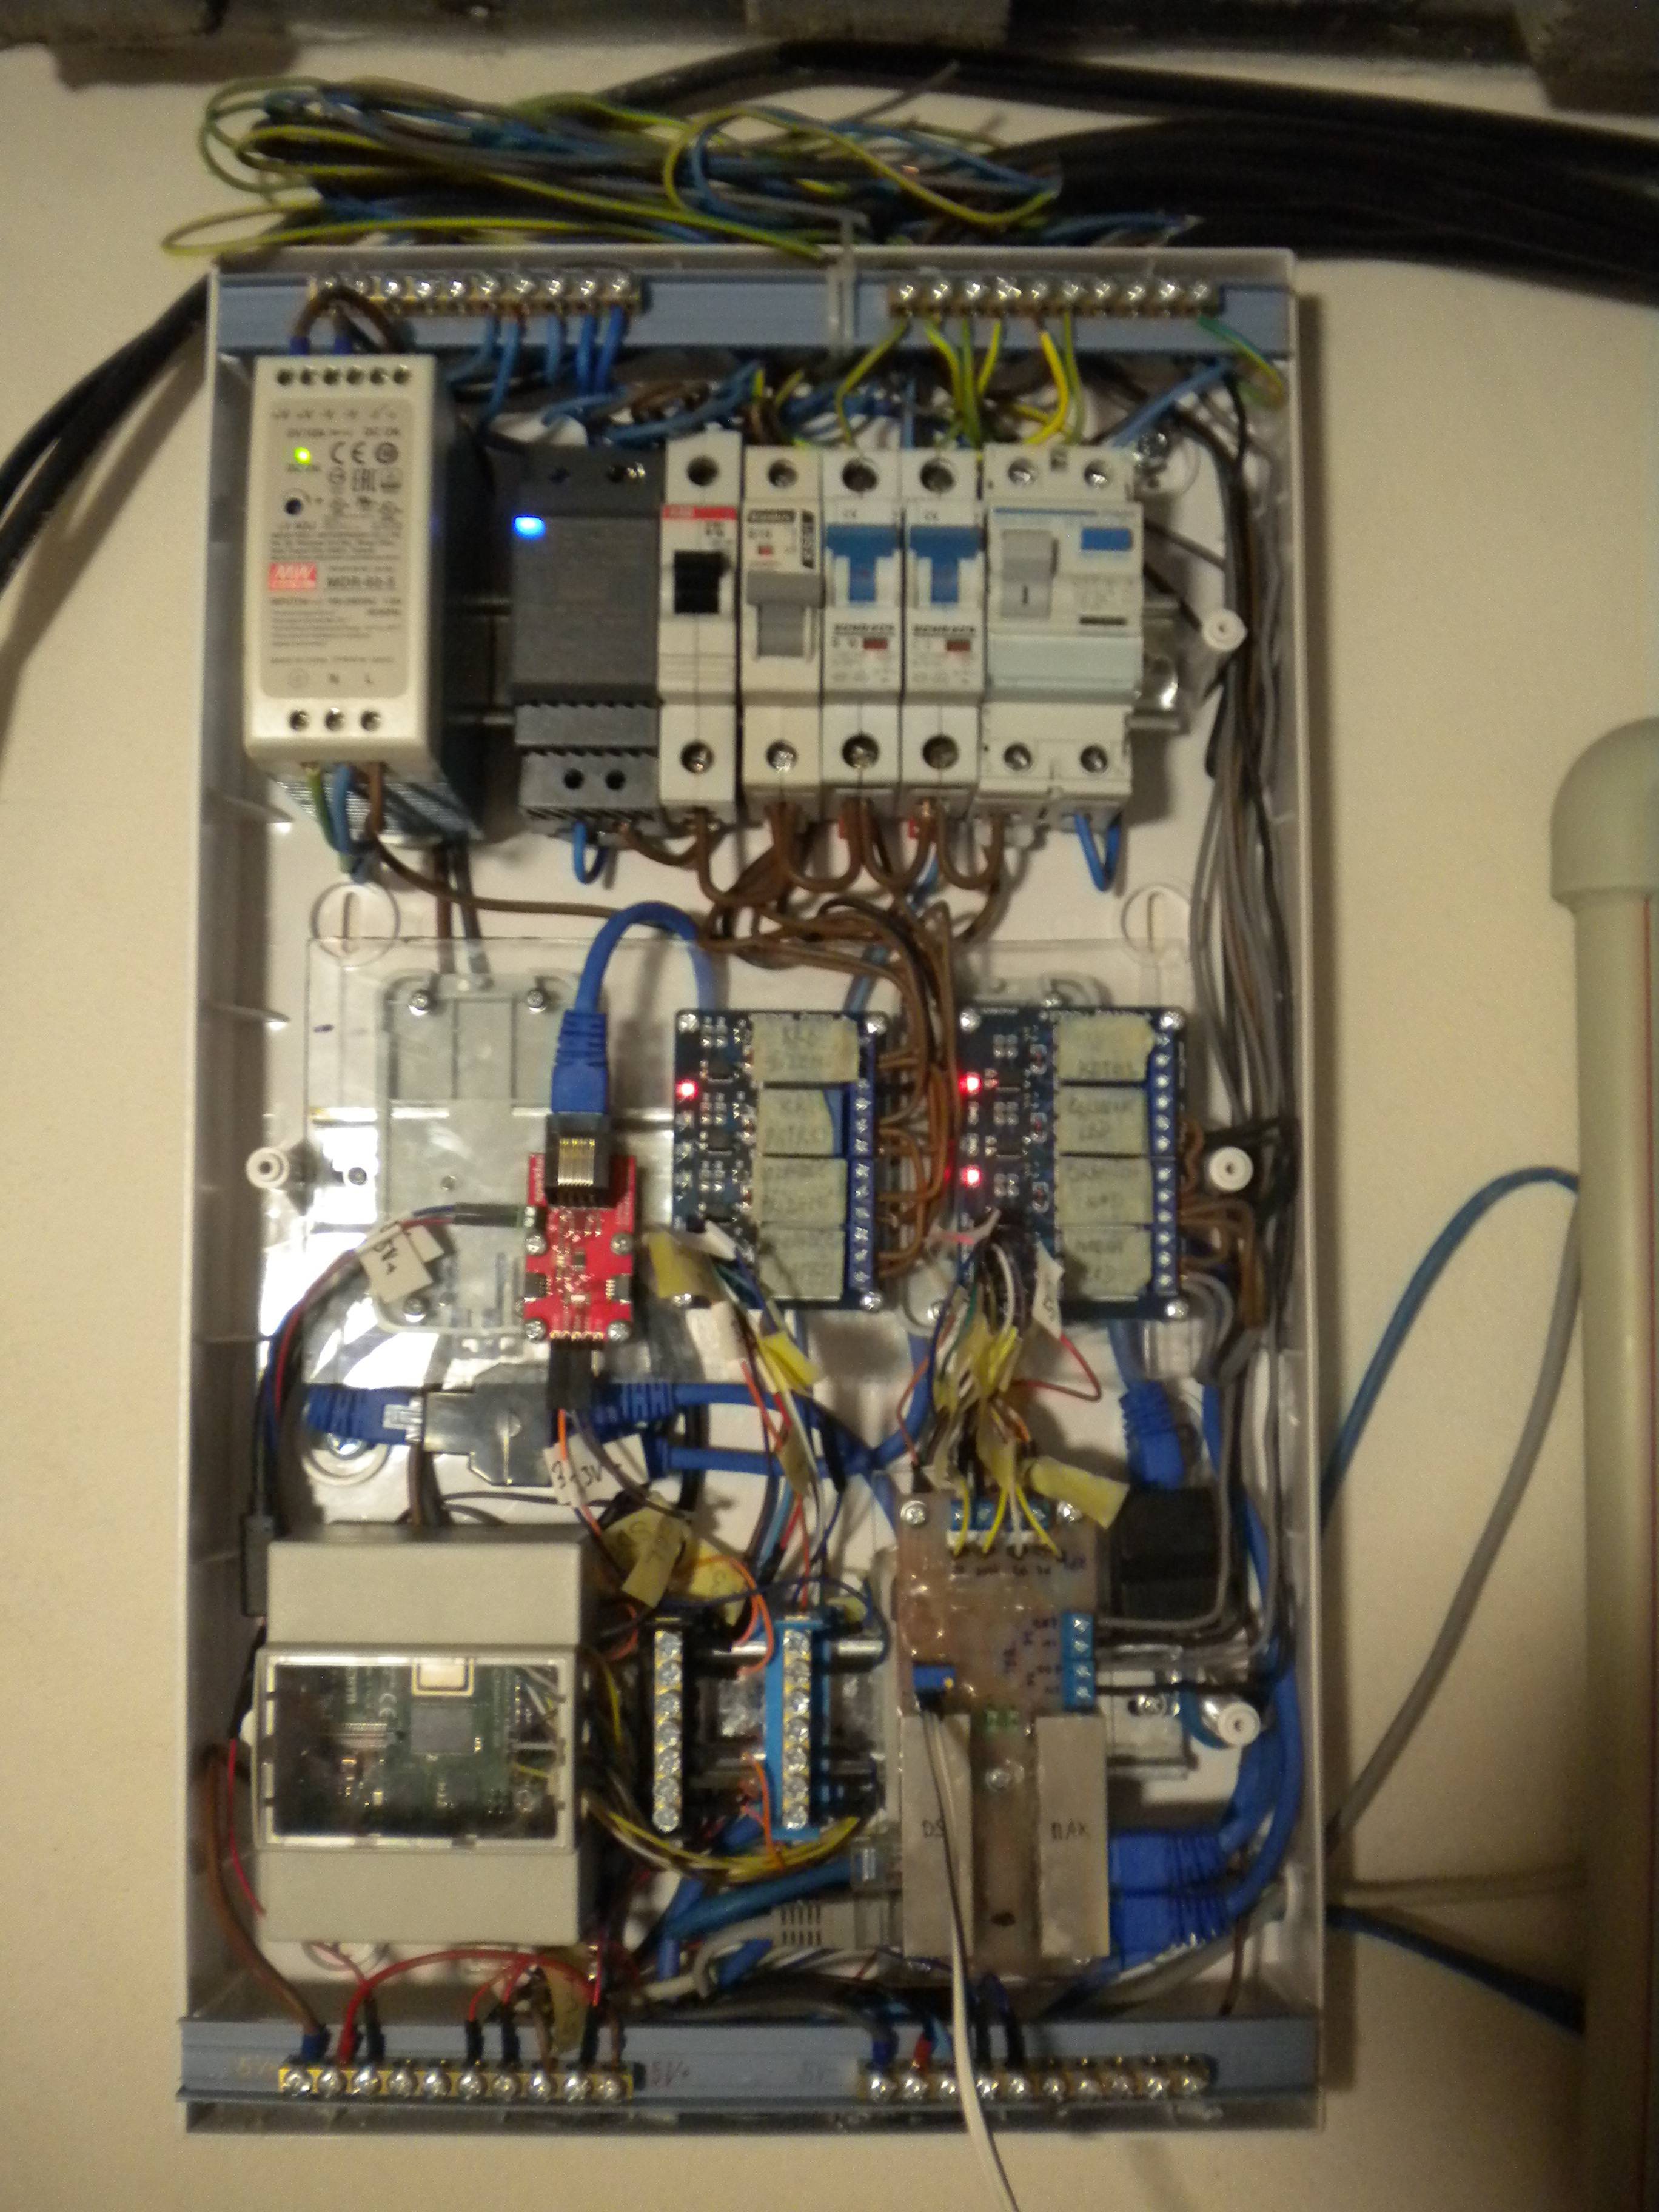
\includegraphics[width=\textwidth]{images/rozvadec-ve-sklepe-s-elektronikou.png}
    \caption{Realizovaný rozvaděč s~elektronikou.}
    \label{fig:rozvadec-ve-sklepe-s-elektronikou}
\end{figure}


\section{Nástěnný snímač prostorové teploty}

Pro snímání prostorové teploty z místností slouží nástěnný snímač prostorové teploty. Tyto zařízení primárně slouží k měření teploty a její následné odesílání do centrální jednotky. Disponují tlačítky pro nastavení požadované teploty (změna teploty s~krokem 0,5 °C) pro danou místnost. Aktuálně naměřenou a požadovanou teplotu zobrazují uživateli přímo na displeji. V případě přenastavení v centrálním systému, dojde k propsání těchto změn přímo na jednotlivé snímací jednotky.  Nástěnný snímač prostorové teploty měří teplotu v místnosti každých 30~sekund. V případě síťového výpadku komunikace se zařízení automaticky snaží připojení obnovit, samotný výpad je signalizován i v centrální jednotce. Jednotky existují ve dvou variantách. První varianta komunikace s centrální jednotkou pomocí Ethernetu a je napájena pomocí aktivního \acrshort{poe} (\textit{\acrlong{poe}}). Druhá varianta komunikuje s centrální jednotkou pomocí bezdrátové sítě WiFi a je napájena pomocí síťového adaptéru. Obě varianty jsou popsány níže v sekci \ref{sec:ethernet-modul} a \ref{sec:wifi-modul}. Celkově je po domě umístěno 6 zařízení s Ethernetem a~4 zařízení s WiFi. DPS byly vlastnoručně navrženy, pro výrobu byla použita firma JLCPCB, součástky byly vlastnoručně osazeny.

\subsection{Varianta s Ethernetem}
\label{sec:ethernet-modul}

\begin{figure}[H]
   \centering
   \def\svgwidth{0.5\columnwidth}
   \input{images/svg/otopna-soustava/vyrez-nastenny-snimac-prostorove-teploty-ethernet.pdf_tex}
    \caption[Výřez pro umístění nástěnných snímačů prostorové teploty (verze Ethernet).]{Výřez z obrázku \ref{fig:otopna-soustava-a-elektronika-rez-domu} – umístění nástěnných snímačů prostorové teploty (verze Ethernet).}
    \label{fig:vyrez-nastenny-snimac-prostorove-teploty-ethernet}
\end{figure}

Na obrázku \ref{fig:vyrez-nastenny-snimac-prostorove-teploty-ethernet} je výřez části z celkového nákresu (obrázek \ref{fig:otopna-soustava-a-elektronika-rez-domu}) pro nástěnné snímače prostorové teploty (verze Ethernet). Na obrázku \ref{fig:blokove-schema-nastenny-snimac-teploty-ethernet} je blokové schéma nástěnného snímače prostorové teploty komunikující pomocí Ethernetu a je napájen pomocí aktivního POE. Snímač je napájen ze zařízení \acrshort{pse} (\textit{\acrlong{pse}}) (jedná se o POE switch MaxLink PSAT-10-8P-250 \cite{maxlink-psat-10-8p-250}), které řídí vykomunikování napájení a~výkonnostní třídy pro koncové zařízení (snímač (\acrshort{pd} (\textit{\acrlong{pd}}))). Jak zařízení PSE, tak PD podporují standart 802.3af \cite{norma-802.3af} respektive 802.3at \cite{norma-802.3at}. Zařízení PD jsou nastavená pro nejnižší definovanou výkonovou třídu 1 (max. výkon PSE pro jednotlivé PD zařízení je 4 W). Pro přenos napětí se využívají tzv. fantomové napětí, kdy v případě využití páru 1,2 a 3,6 se stejnosměrné napětí vyvede ze středu transformátoru. Další možností je využití volných párů 4,5 a 7,8 (zejména při rychlosti 10 nebo 100~Mbit/s (využity pro přenos dat 2 páry)). Vstupní napětí z PSE (44–57 V v~závislosti na délce kabelu UTP a~ztrátách) prochází přes diodový usměrňovač (nezávislost kladného pólu zdroje a země). Je zde řídící obvod TPS23753A \cite{tps23753a}, který zajišťuje komunikaci/rozhraní pro správné nastavení a povolení napětí z PSE, dále zajišťuje řízení převodu vstupního napětí na výstupní napětí 5~V (DC-DC měnič), je zapojen v~topologie Flyback (využívá tedy vázaný induktor). Zpětná vazba je řešena pomocí optické zpětné vazby s nastavitelnou Zenerovou diodou TLV431A \cite{tlv431a} v~zapojení komparátoru. Při návrh zdrojové části zařízení jsem vycházel z referenčního návrhu od výrobce Texas Instruments pro integrovaný obvod TPS23753A.

Zařízení v provozu je primárně  napájeno pomocí 5 V, v případě programování zařízení je možné použít programovací konektor s napájecím pinem pro 5 V. Pokud je k~dispozici POE, dojde zablokování napájení z programovacího konektoru (pomocí MOSFETu s~kanálem P). Napětí 5 V je následně vedeno do dvou \acrshort{ldo} (\textit{\acrlong{ldo}}) regulátorů. Jeden slouží pouze pro napájení ESP32 \cite{esp32-wrover-ie} modulu, druhý je pro napájení zbylých periferií (displej, tlačítka, teplotní senzor, obvod pro fyzickou vrstvu Ethernetu W5500 \cite{w5500}). Důvodem rozdělení je proudové rozdělení jednotlivých regulátorů a tedy i jejich ztrátové teplo. Vzhledem k parametrům udávané výrobcem modulu ESP32 je možné max. proudový odběr až 0,5~A (proto byl vybrán regulátor, který toto zatížení dlouhodobě zvládne při daném úbytku napětí i když se reálně nepředpokládá, že k tomuto zatížení dojde). Dále bylo zohledněno, pokud by došlo k ESD události (jedná se o~zařízení na které uživatelé sahají), tak je žádoucí, aby došlo maximálně k~restartu periferií a ne k restartu samotného ESP32 modulu. 

Pro programování modulu je zde konektor pro připojení externího modulu (viz část \ref{sec:prevodnik-usb-uart-cp2102n}), kde jsou piny pro TX/RX signál z UART a signály na automatický reset a boot modulu a piny pro napájení 5 V a země. Dále jsou zde přímo na DPS umístěná tlačítka pro boot a reset ESP32 modulu bez závislosti připojení programovacího modulu (lze tedy programovat i jinými moduly, které nemají automatický reset a boot). 

Samotné zařízení disponujeme ohranými transily na místech konektorů a~částí, které jsou přímo v kontaktu s uživatelem. Samotný obvod pro POE též disponuje proudovou a teplotní ochranou. LDO regulátory disponují detekcí nízkého vstupního napětí pro úspěšné spuštění, teplotní pojistkou a ochranou při zvýšení výstupního napětí vůči vstupnímu. 

Pro zobrazování aktuální a požadované teploty jsem zvolil barevný TFT displej velikosti 2.2" (240×320 pixelů) s řadičem ILI9341 \cite{lcd-ili9341}. Displej je připojen k~ESP32 modulu pomocí SPI sběrnice. Displej disponuje možností ovládání podsvícení pomocí PWM. Pro fyzickou vrstvu slouží obvod W5500, který implementuje ethernetový řadič s integrovaným TCP/IP. Obvod je s modulem ESP32 připojen pomocí SPI sběrnice. Pro snímání teploty slouží teplotní senzor DS18B20 (viz sekce \ref{sec:teplotni-senzory-pro-krby}). V neposlední řadě jsou zde tři tlačítka pro nastavení požadované teploty a~vyvolání nabídky menu.

Modul ESP32 disponuje rozhraním \acrshort{rmii} (\textit{\acrlong{rmii}}), který má složitější softwarovou implementaci a využívá větší počet pinů. Proto jsem zvolil integrovaný obvod W5500. Použití i využití následných knihoven bylo mnohem jednodušší. Vzhledem k malému vytížení komunikace je tento obvod dostačující. Pro komunikace mezi modulem ESP32 a displejem a obvodem W5500 jsou využity dvě nezávislé SPI sběrnice. 

V příloze \ref{app:nastenny-snimac-prostorove-teploty-ethernet} je schéma snímací jednotky. Na obrázku \ref{fig:dps-nastenny-snimac-prostorove-teploty-ethernet-vrchni-cast} je vrchní část realizované DPS pro snímací jednotku. Pro lepší galvanické oddělení jsou vyfrézované drážky. Dále na obrázku \ref{fig:dps-nastenny-snimac-prostorove-teploty-ethernet-vrchni-cast-displej} je DPS s osazeným displejem. Na obrázku \ref{fig:dps-nastenny-snimac-prostorove-teploty-ethernet-spodni-cast} je spodní část DPS. Kompletní zařízení včetně umístění do krabičky a popis samotné krabičky je v části \ref{sec:krabicka-pro-nastenny-snimac-prostorove-teploty}.



\begin{figure}[H]
    \centering
    \def\svgwidth{\columnwidth}
    \input{images/svg/blokove-schema-nastenny-snimac-teploty-ethernet.pdf_tex}
    \caption[]{Blokové schéma nástěnného snímače prostorové teploty (verze Ethernet).}
    \label{fig:blokove-schema-nastenny-snimac-teploty-ethernet}
\end{figure}


\begin{figure}[H]
\centering
\begin{subfigure}{.5\textwidth}
  \centering
  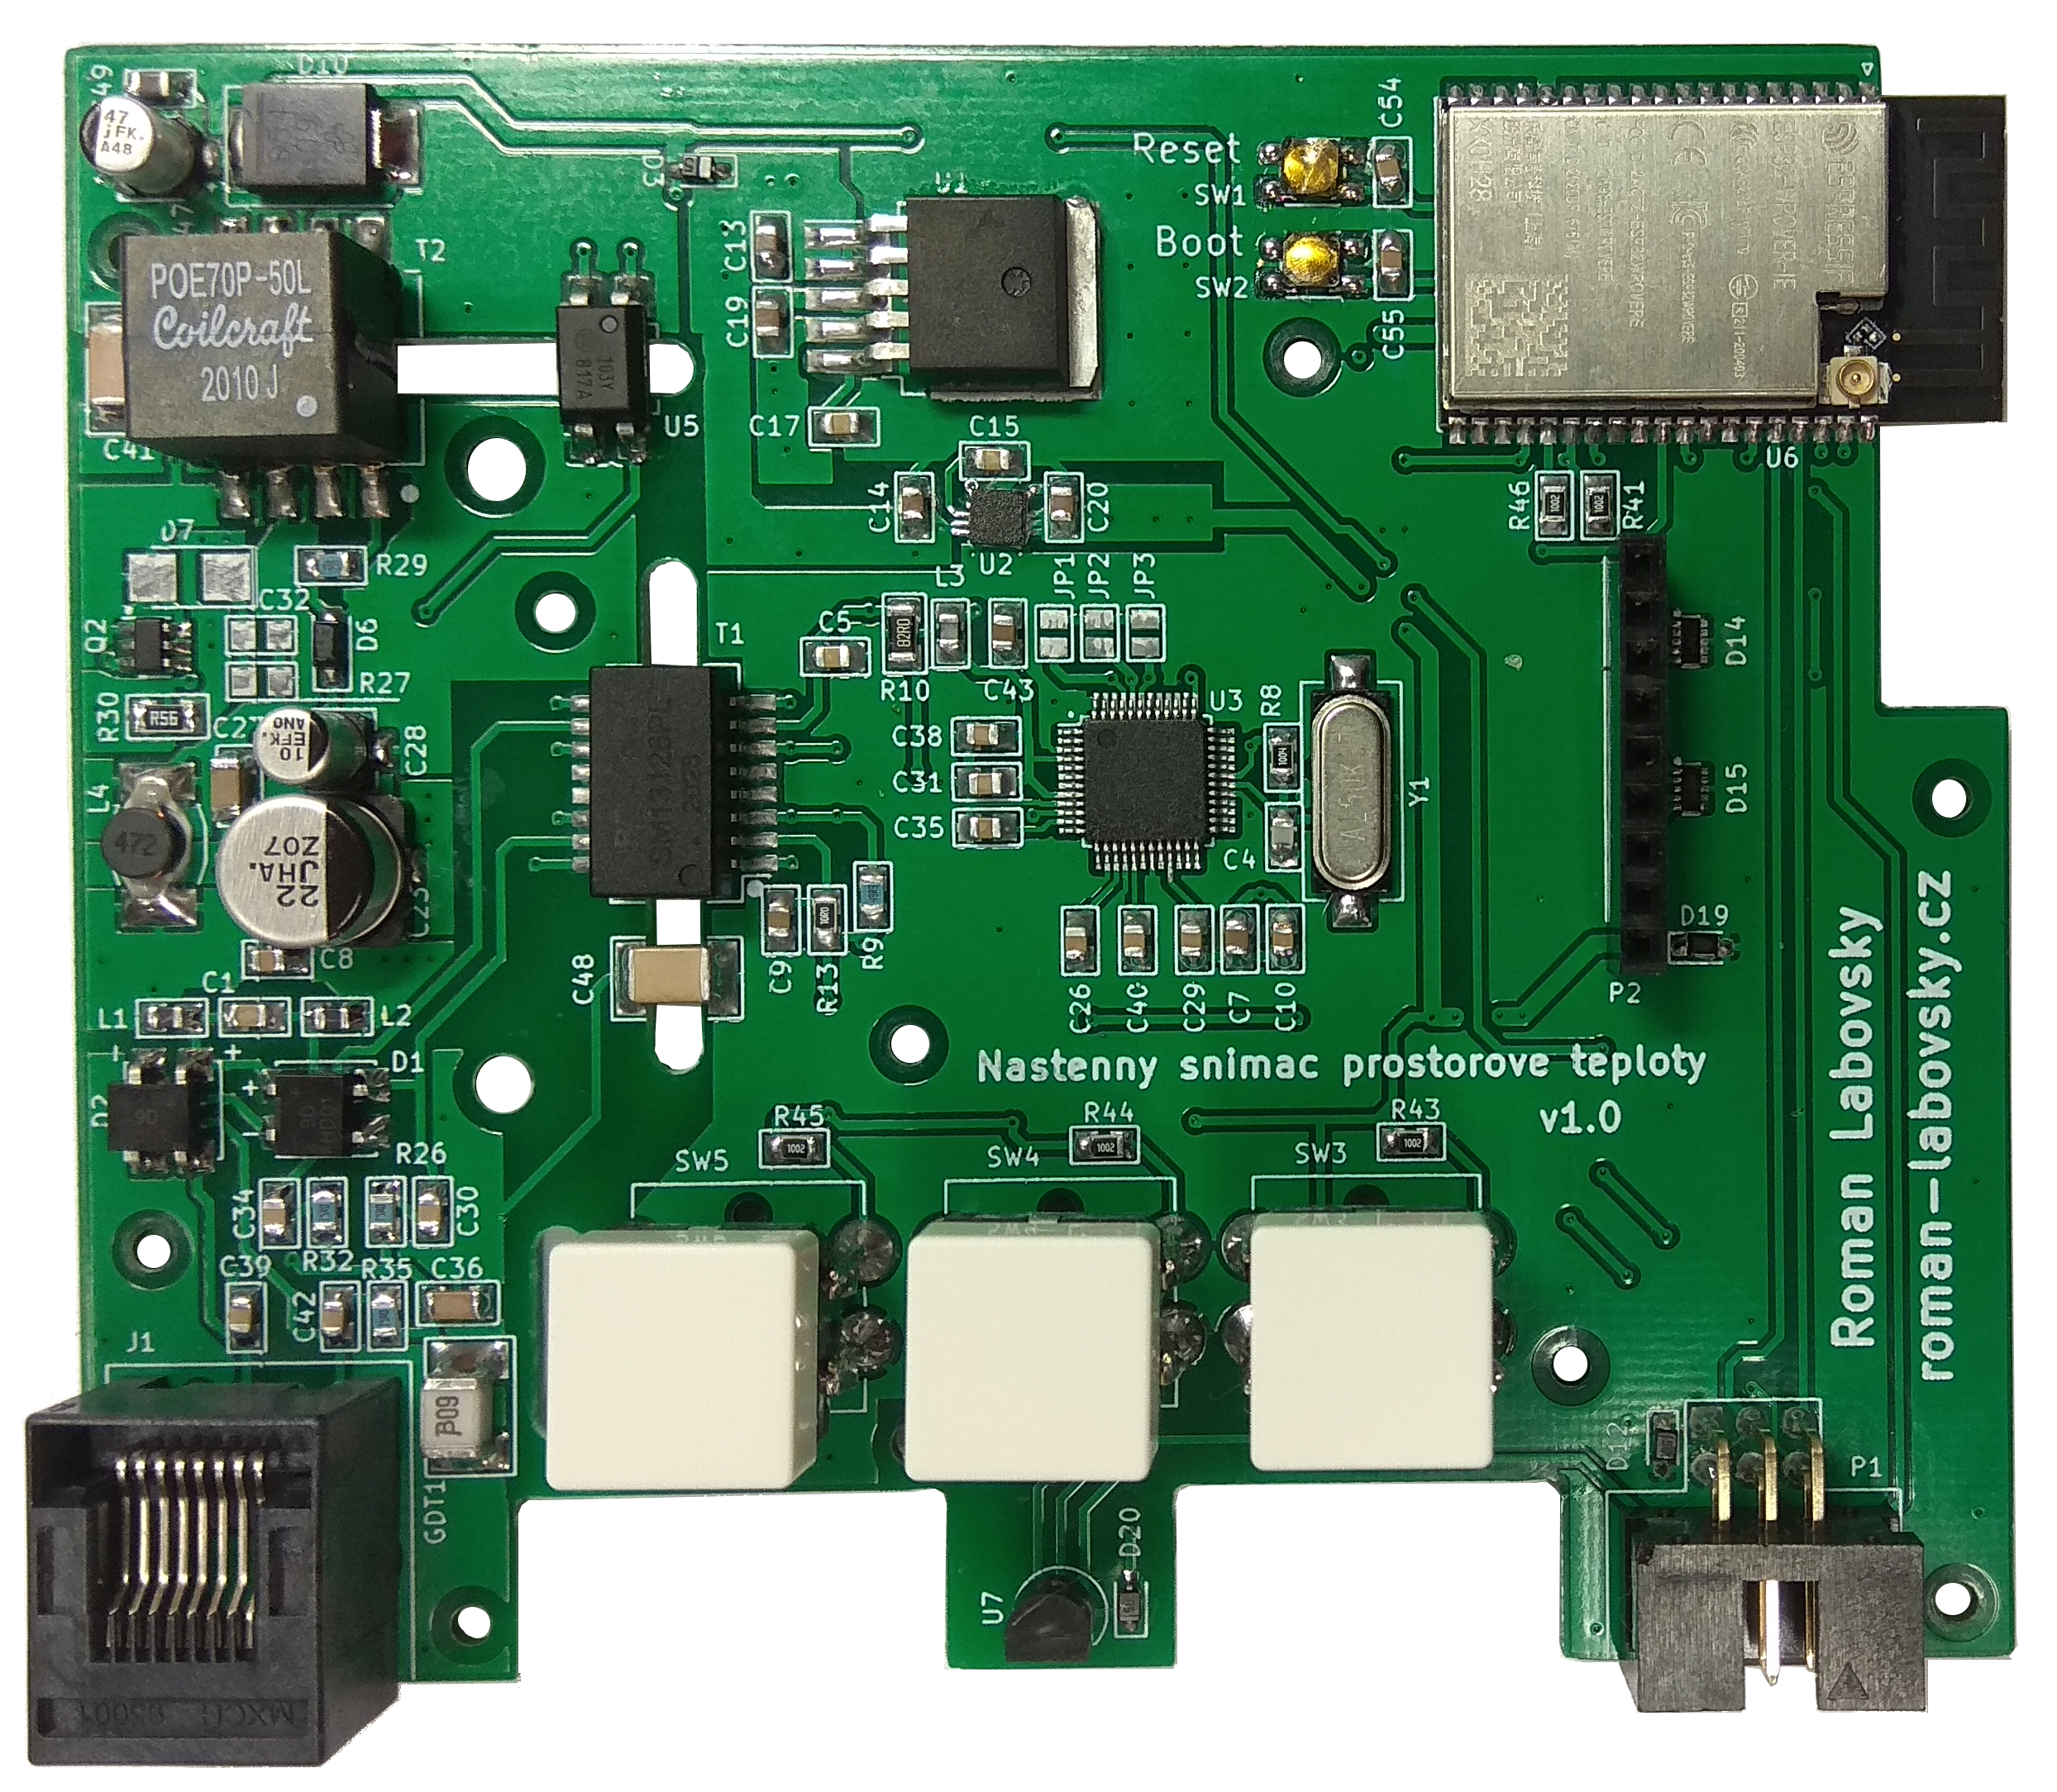
\includegraphics[width=\textwidth]{images/nastenny-snimac-prostorove-teploty-ethernet/dps-nastenny-snimac-prostorove-teploty-ethernet-vrchni-cast.png}
  \caption{Vrchní strana.}
  \label{fig:dps-nastenny-snimac-prostorove-teploty-ethernet-vrchni-cast}
\end{subfigure}%
\begin{subfigure}{.5\textwidth}
  \centering
  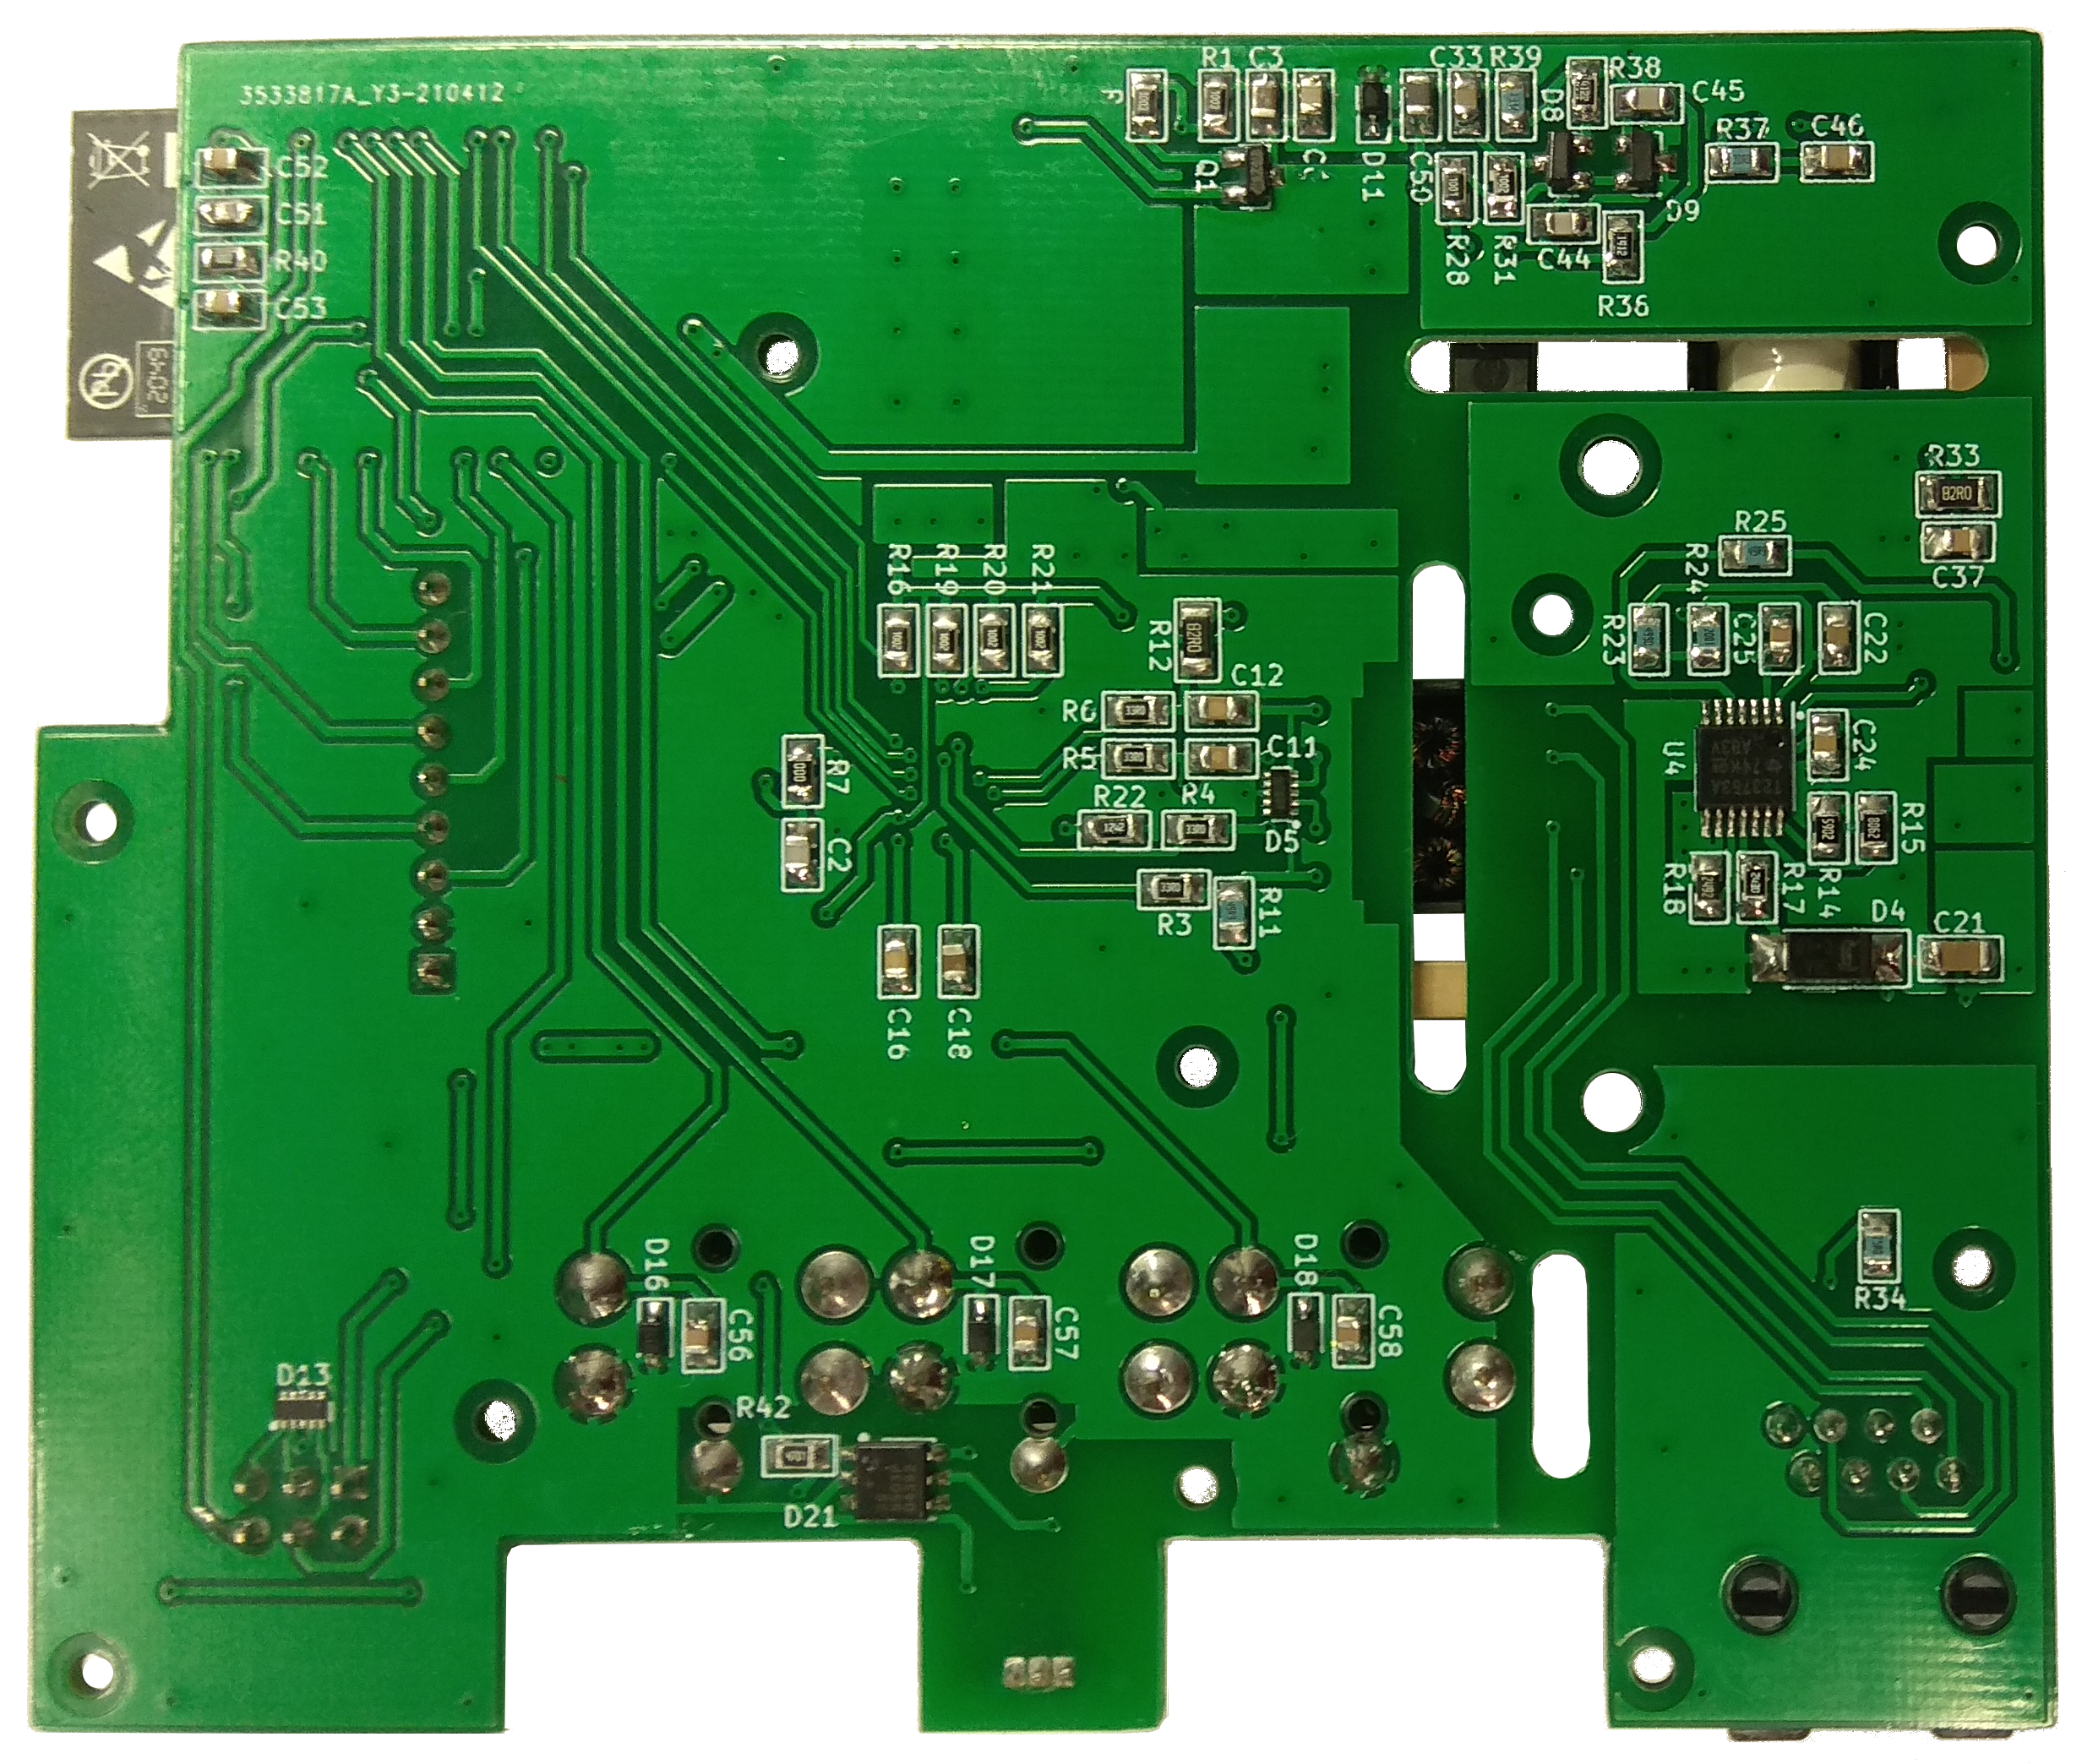
\includegraphics[width=\textwidth]{images/nastenny-snimac-prostorove-teploty-ethernet/dps-nastenny-snimac-prostorove-teploty-ethernet-spodni-cast.png}
  \caption{Spodní strana.}
  \label{fig:dps-nastenny-snimac-prostorove-teploty-ethernet-spodni-cast}
\end{subfigure}
\caption{DPS nástěnného snímače prostorové teploty (verze Ethernet).}
\label{fig:dps-nastenny-snimac-prostorove-teploty-ethernet}
\end{figure}


\begin{figure}[H]
    \centering
    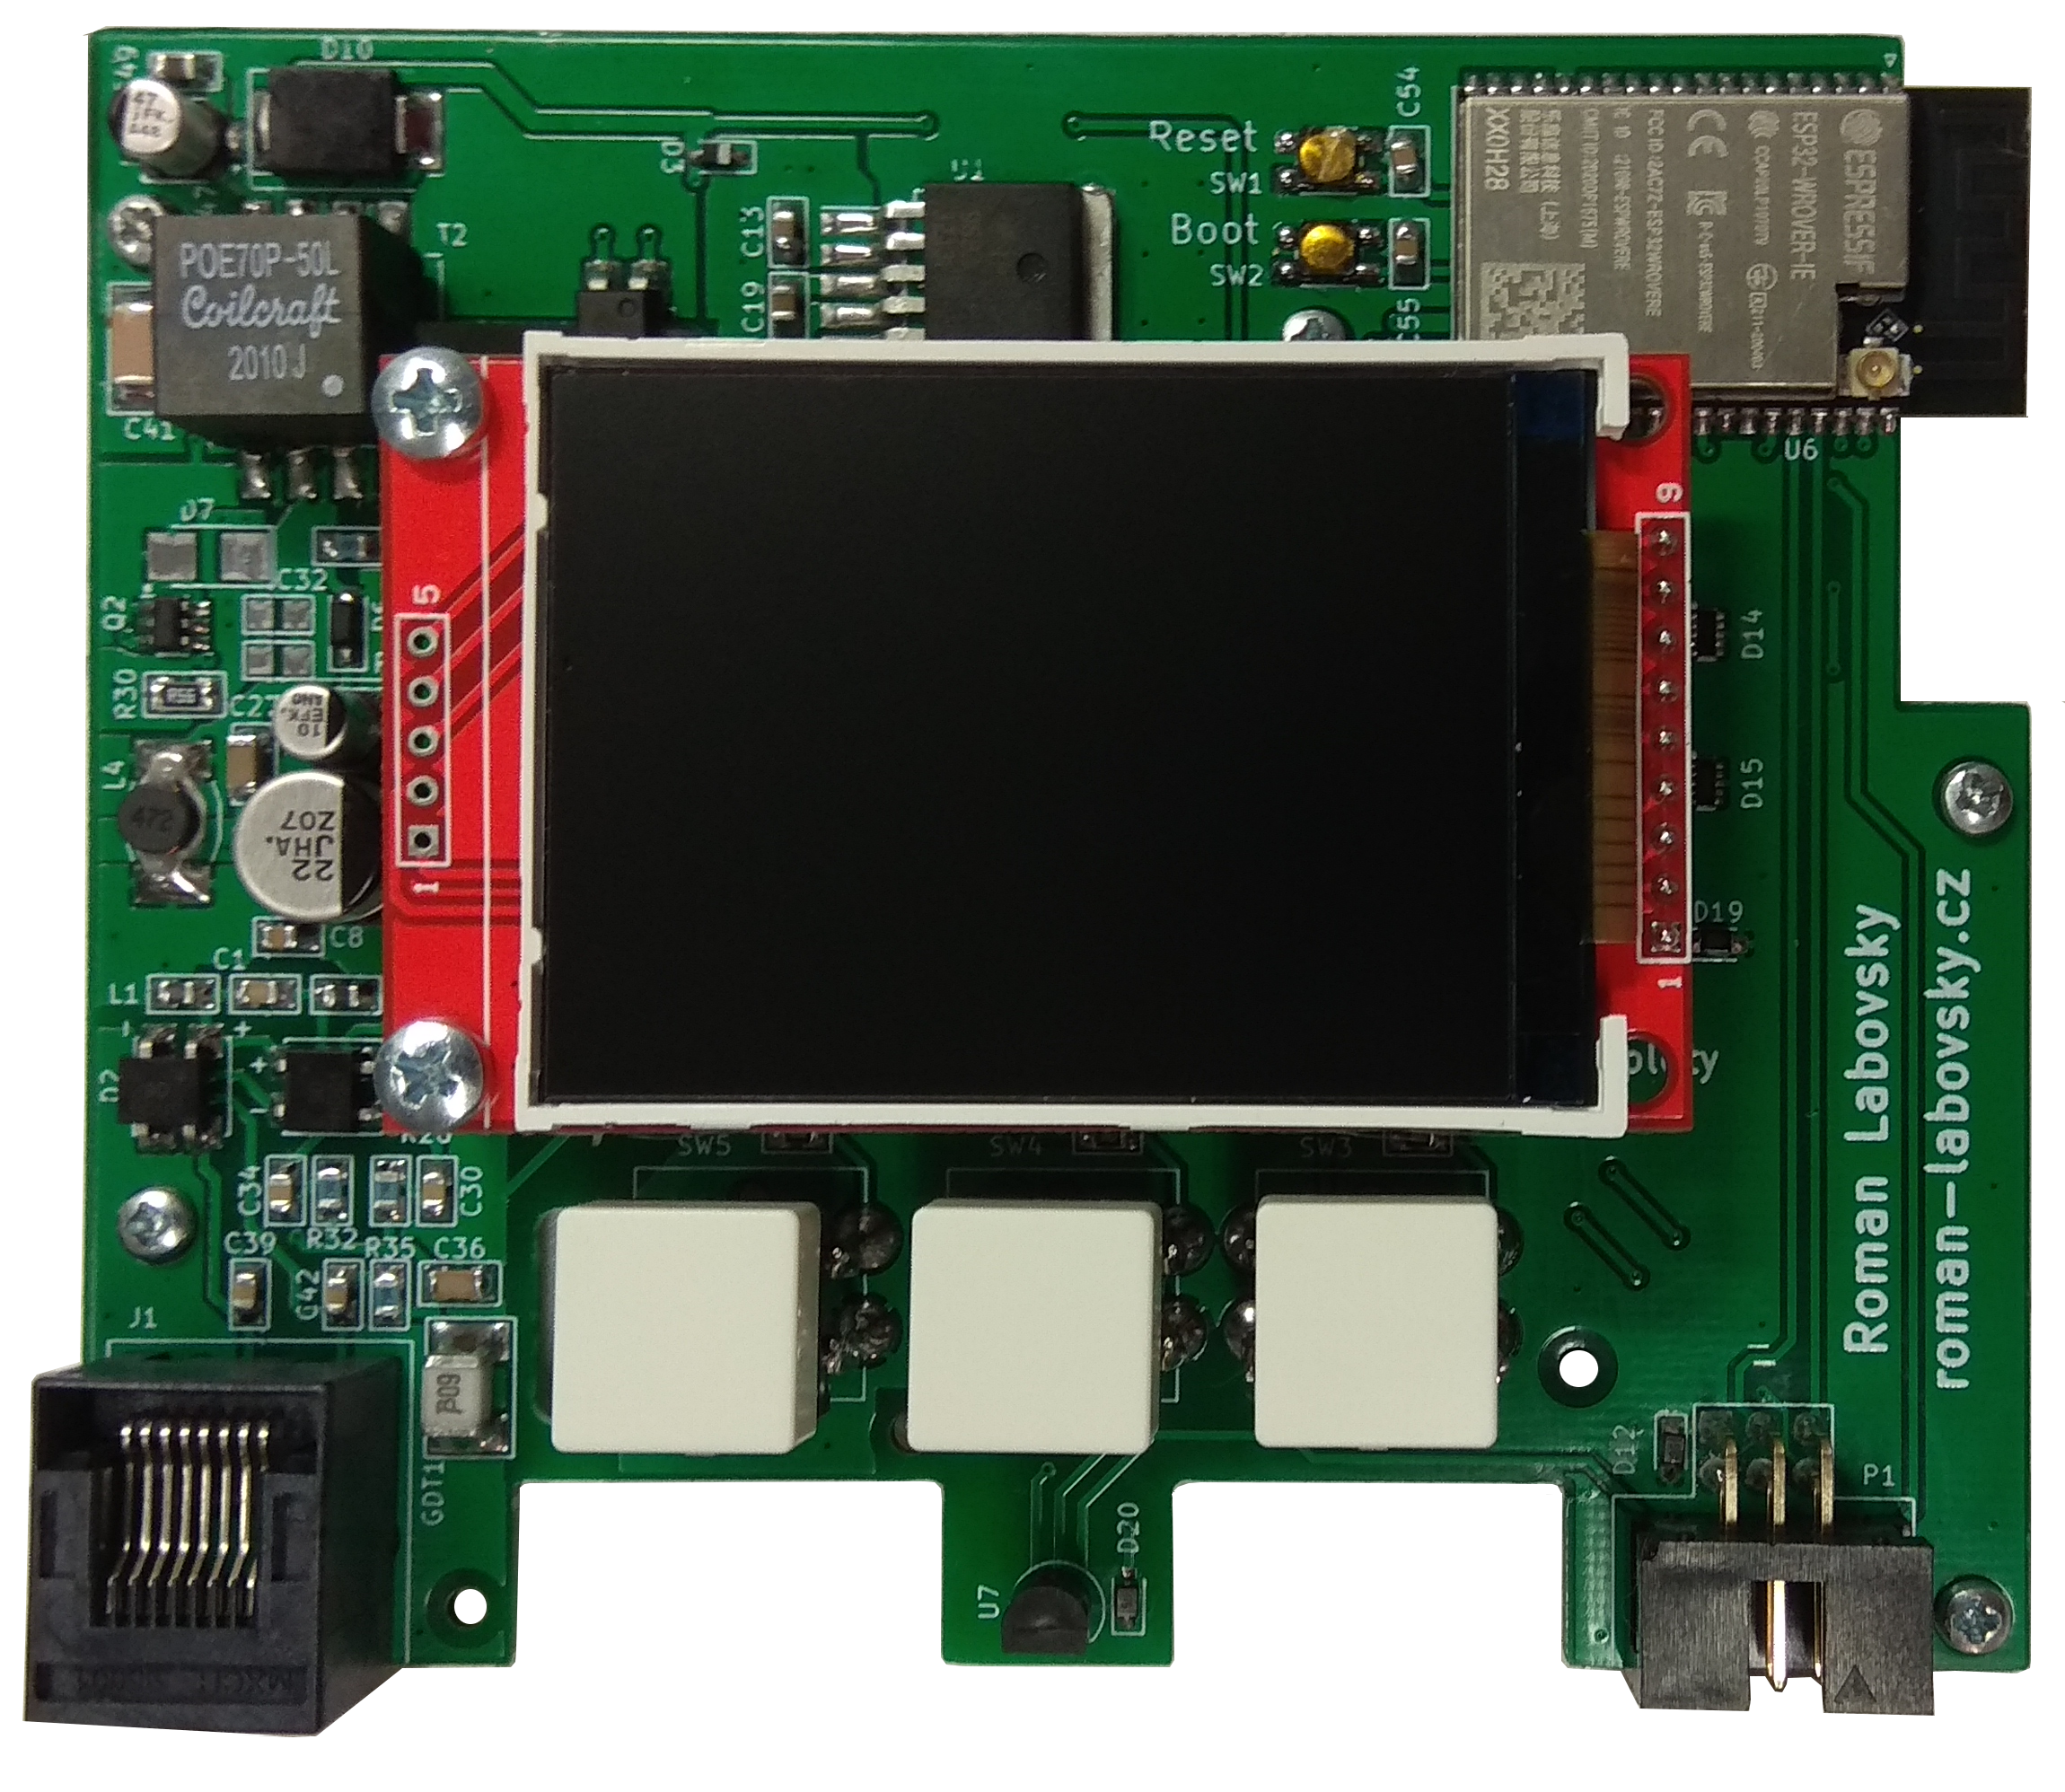
\includegraphics[width=0.88\textwidth]{images/nastenny-snimac-prostorove-teploty-ethernet/dps-nastenny-snimac-prostorove-teploty-ethernet-vrchni-cast-displej.png}
    \caption{DPS nástěnného snímače prostorové teploty (verze Ethernet) s~displejem, vrchní strana.}
    \label{fig:dps-nastenny-snimac-prostorove-teploty-ethernet-vrchni-cast-displej}
\end{figure}



\subsection{Varianta s WiFi}
\label{sec:wifi-modul}


\begin{figure}[H]
   \centering
   \def\svgwidth{0.5\columnwidth}
   \input{images/svg/otopna-soustava/vyrez-nastenny-snimac-prostorove-teploty-wifi.pdf_tex}
    \caption[Výřez umístění nástěnných snímačů prostorové teploty (verze WiFi).]{Výřez z obrázku \ref{fig:otopna-soustava-a-elektronika-rez-domu} – umístění nástěnných snímačů prostorové teploty (verze WiFi).}
    \label{fig:vyrez-nastenny-snimac-prostorove-teploty-wifi}
\end{figure}

Na obrázku \ref{fig:vyrez-nastenny-snimac-prostorove-teploty-wifi} je výřez části z celkového nákresu (obrázek \ref{fig:otopna-soustava-a-elektronika-rez-domu}) systému znázorňující umístění nástěnných snímačů prostorové teploty (verze WiFi). Na obrázku \ref{fig:blokove-schema-nastenny-snimac-teploty-wifi} je blokové schéma nástěnného snímače prostorové teploty komunikující pomocí WiFi a je napájen pomocí síťového adaptéru (Mean Well GSM06E05-P1J \cite{gsm06e05-p1j}). Oproti verzi z \ref{sec:ethernet-modul} chybí celá část tykající se POE napájení a také obvod W5500 implementující ethernetovou komunikaci. Zbylé části jsou totožné jako v části \ref{sec:ethernet-modul}.

V příloze \ref{app:nastenny-snimac-prostorove-teploty-wifi} je schéma snímací jednotky. Na obrázku \ref{fig:dps-nastenny-snimac-prostorove-teploty-wifi-vrchni-cast} je vrchní část realizované DPS pro snímací jednotku. Dále na obrázku \ref{fig:dps-nastenny-snimac-prostorove-teploty-wifi-vrchni-cast-displej} je DPS s osazeným displejem. Na obrázku \ref{fig:dps-nastenny-snimac-prostorove-teploty-wifi-spodni-cast} je spodní část DPS. Kompletní zařízení včetně umístění do krabičky a popis samotné krabičky je v části \ref{sec:krabicka-pro-nastenny-snimac-prostorove-teploty}.

\begin{figure}[H]
    \centering
    \def\svgwidth{\columnwidth}
    \input{images/svg/blokove-schema-nastenny-snimac-teploty-wifi.pdf_tex}
    \caption[]{Blokové schéma nástěnného snímače prostorové teploty (verze WiFi).}
    \label{fig:blokove-schema-nastenny-snimac-teploty-wifi}
\end{figure}


\begin{figure}[H]
\centering
\begin{subfigure}{.5\textwidth}
  \centering
    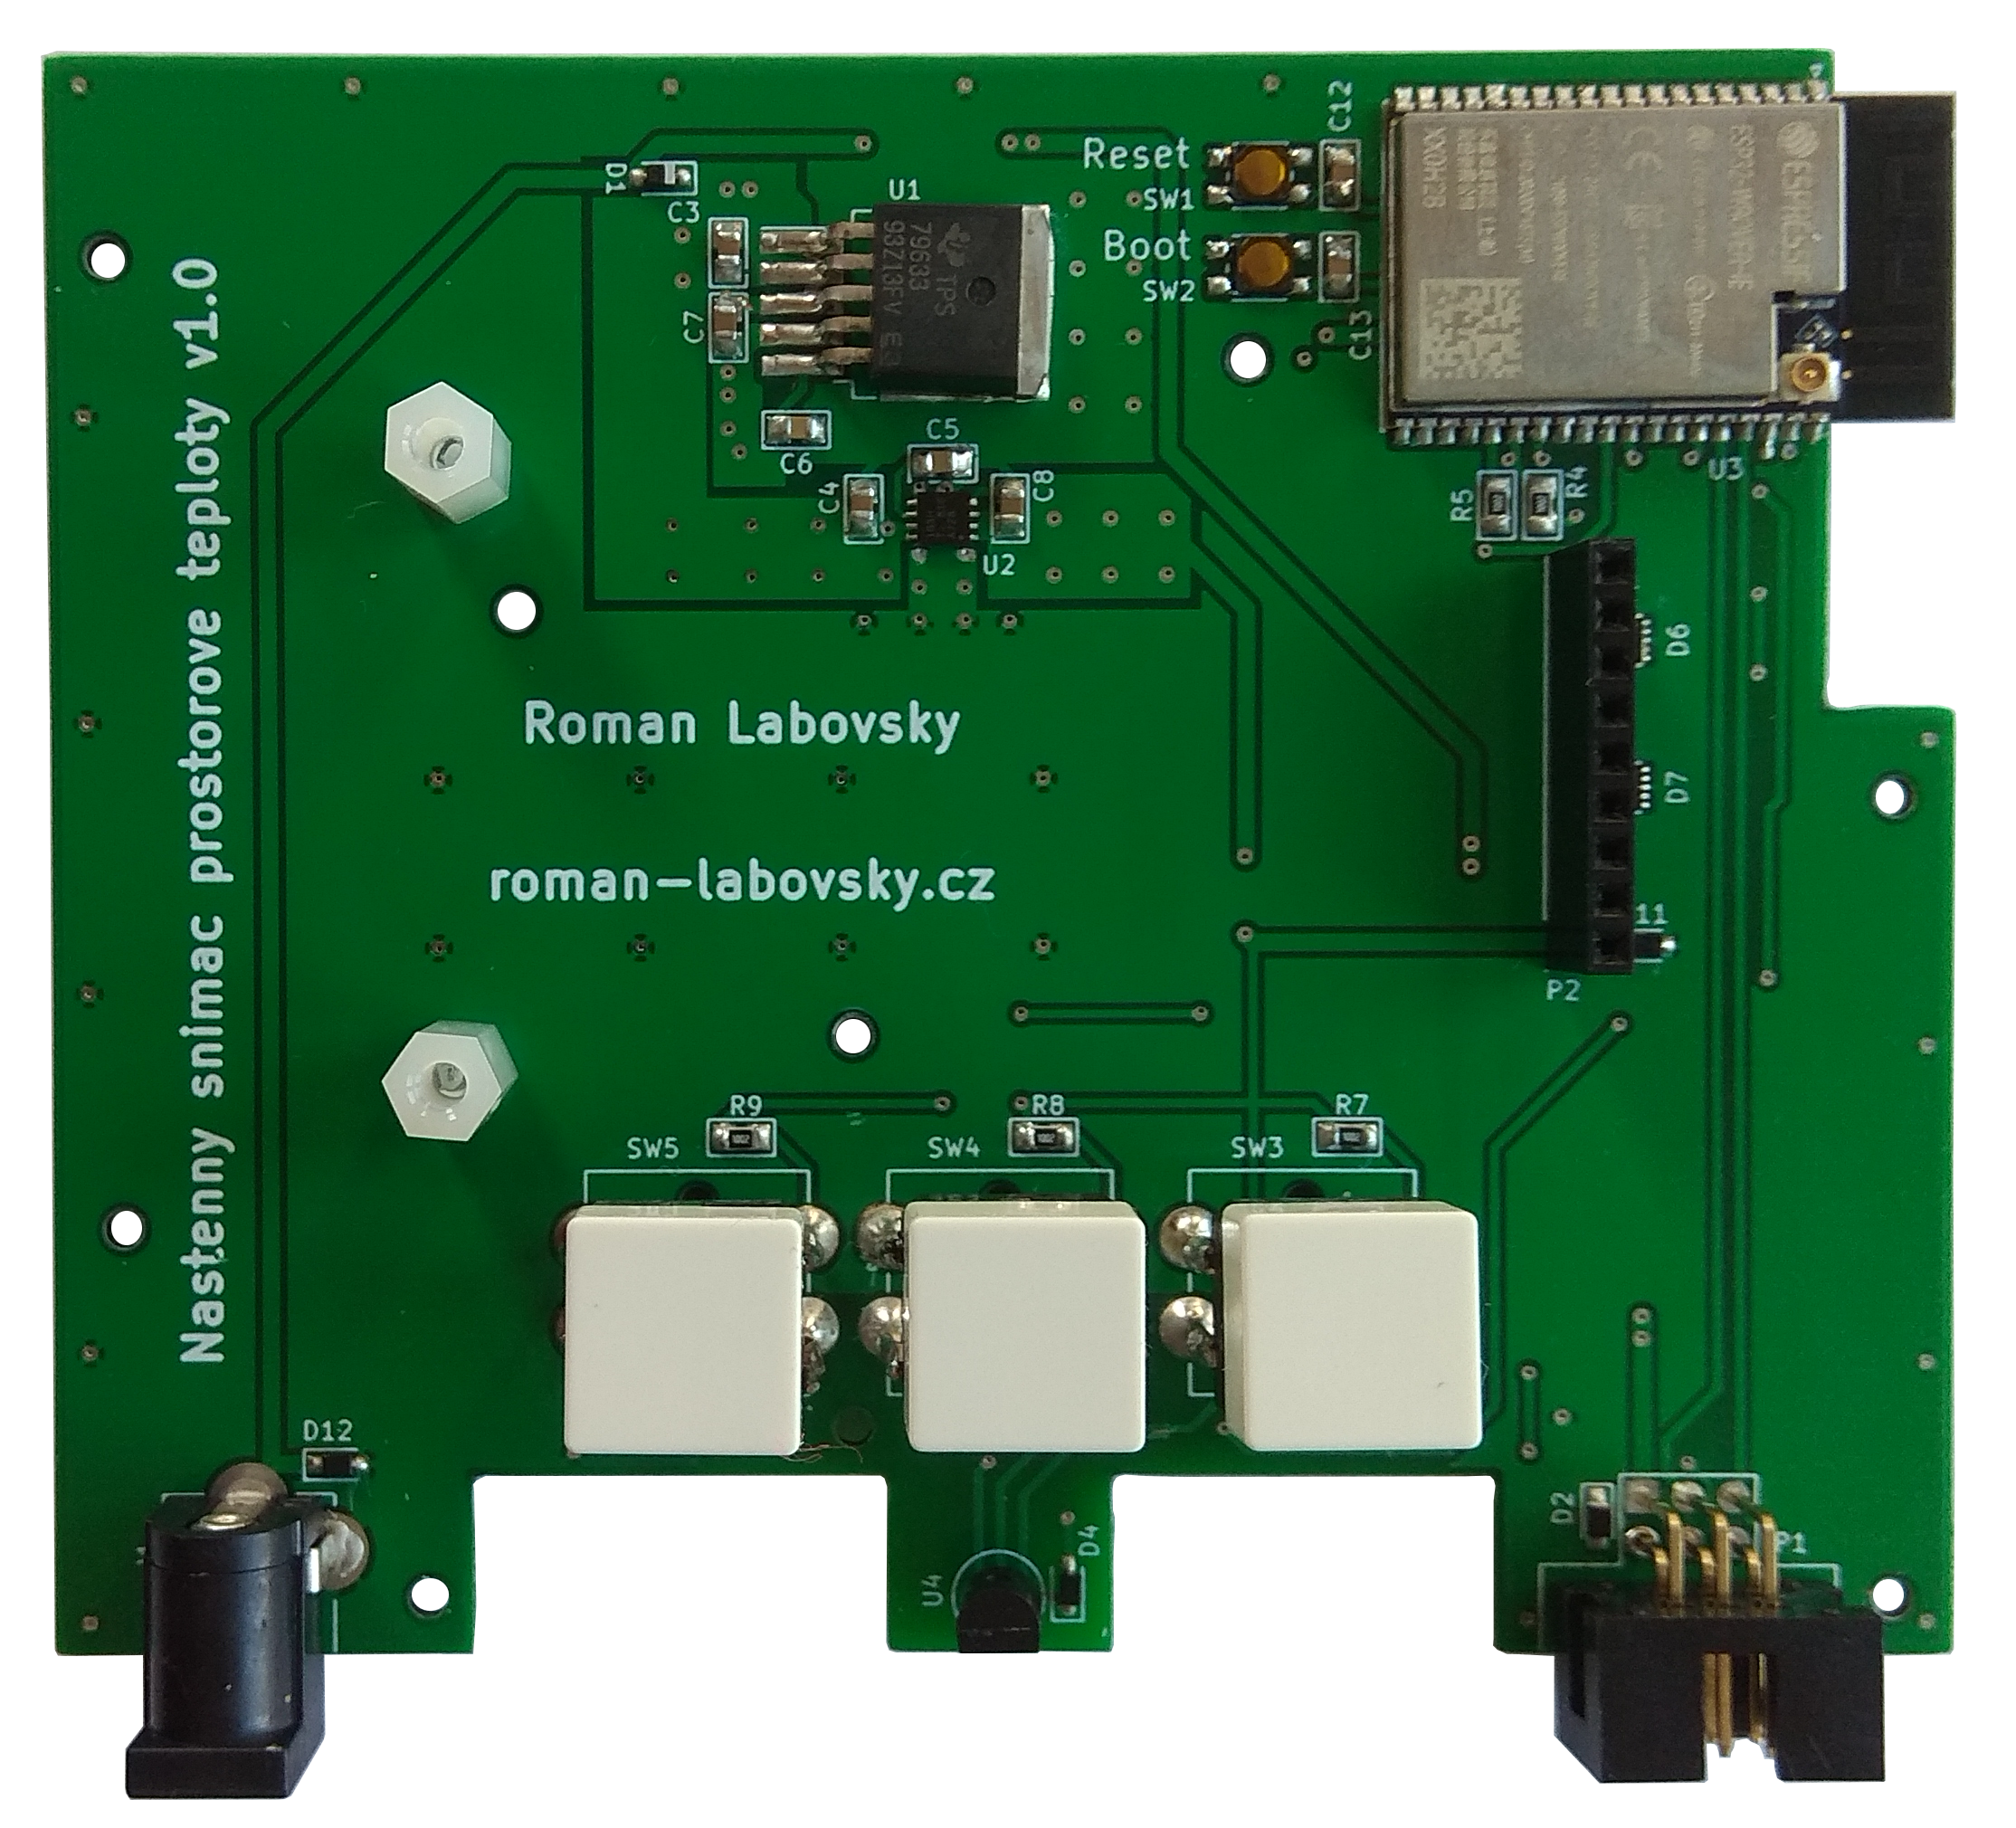
\includegraphics[width=\textwidth]{images/nastenny-snimac-prostorove-teploty-wifi/dps-nastenny-snimac-prostorove-teploty-wifi-vrchni-cast.png}
    \caption{Vrchní strana.}
    \label{fig:dps-nastenny-snimac-prostorove-teploty-wifi-vrchni-cast}
\end{subfigure}%
\begin{subfigure}{.5\textwidth}
  \centering
    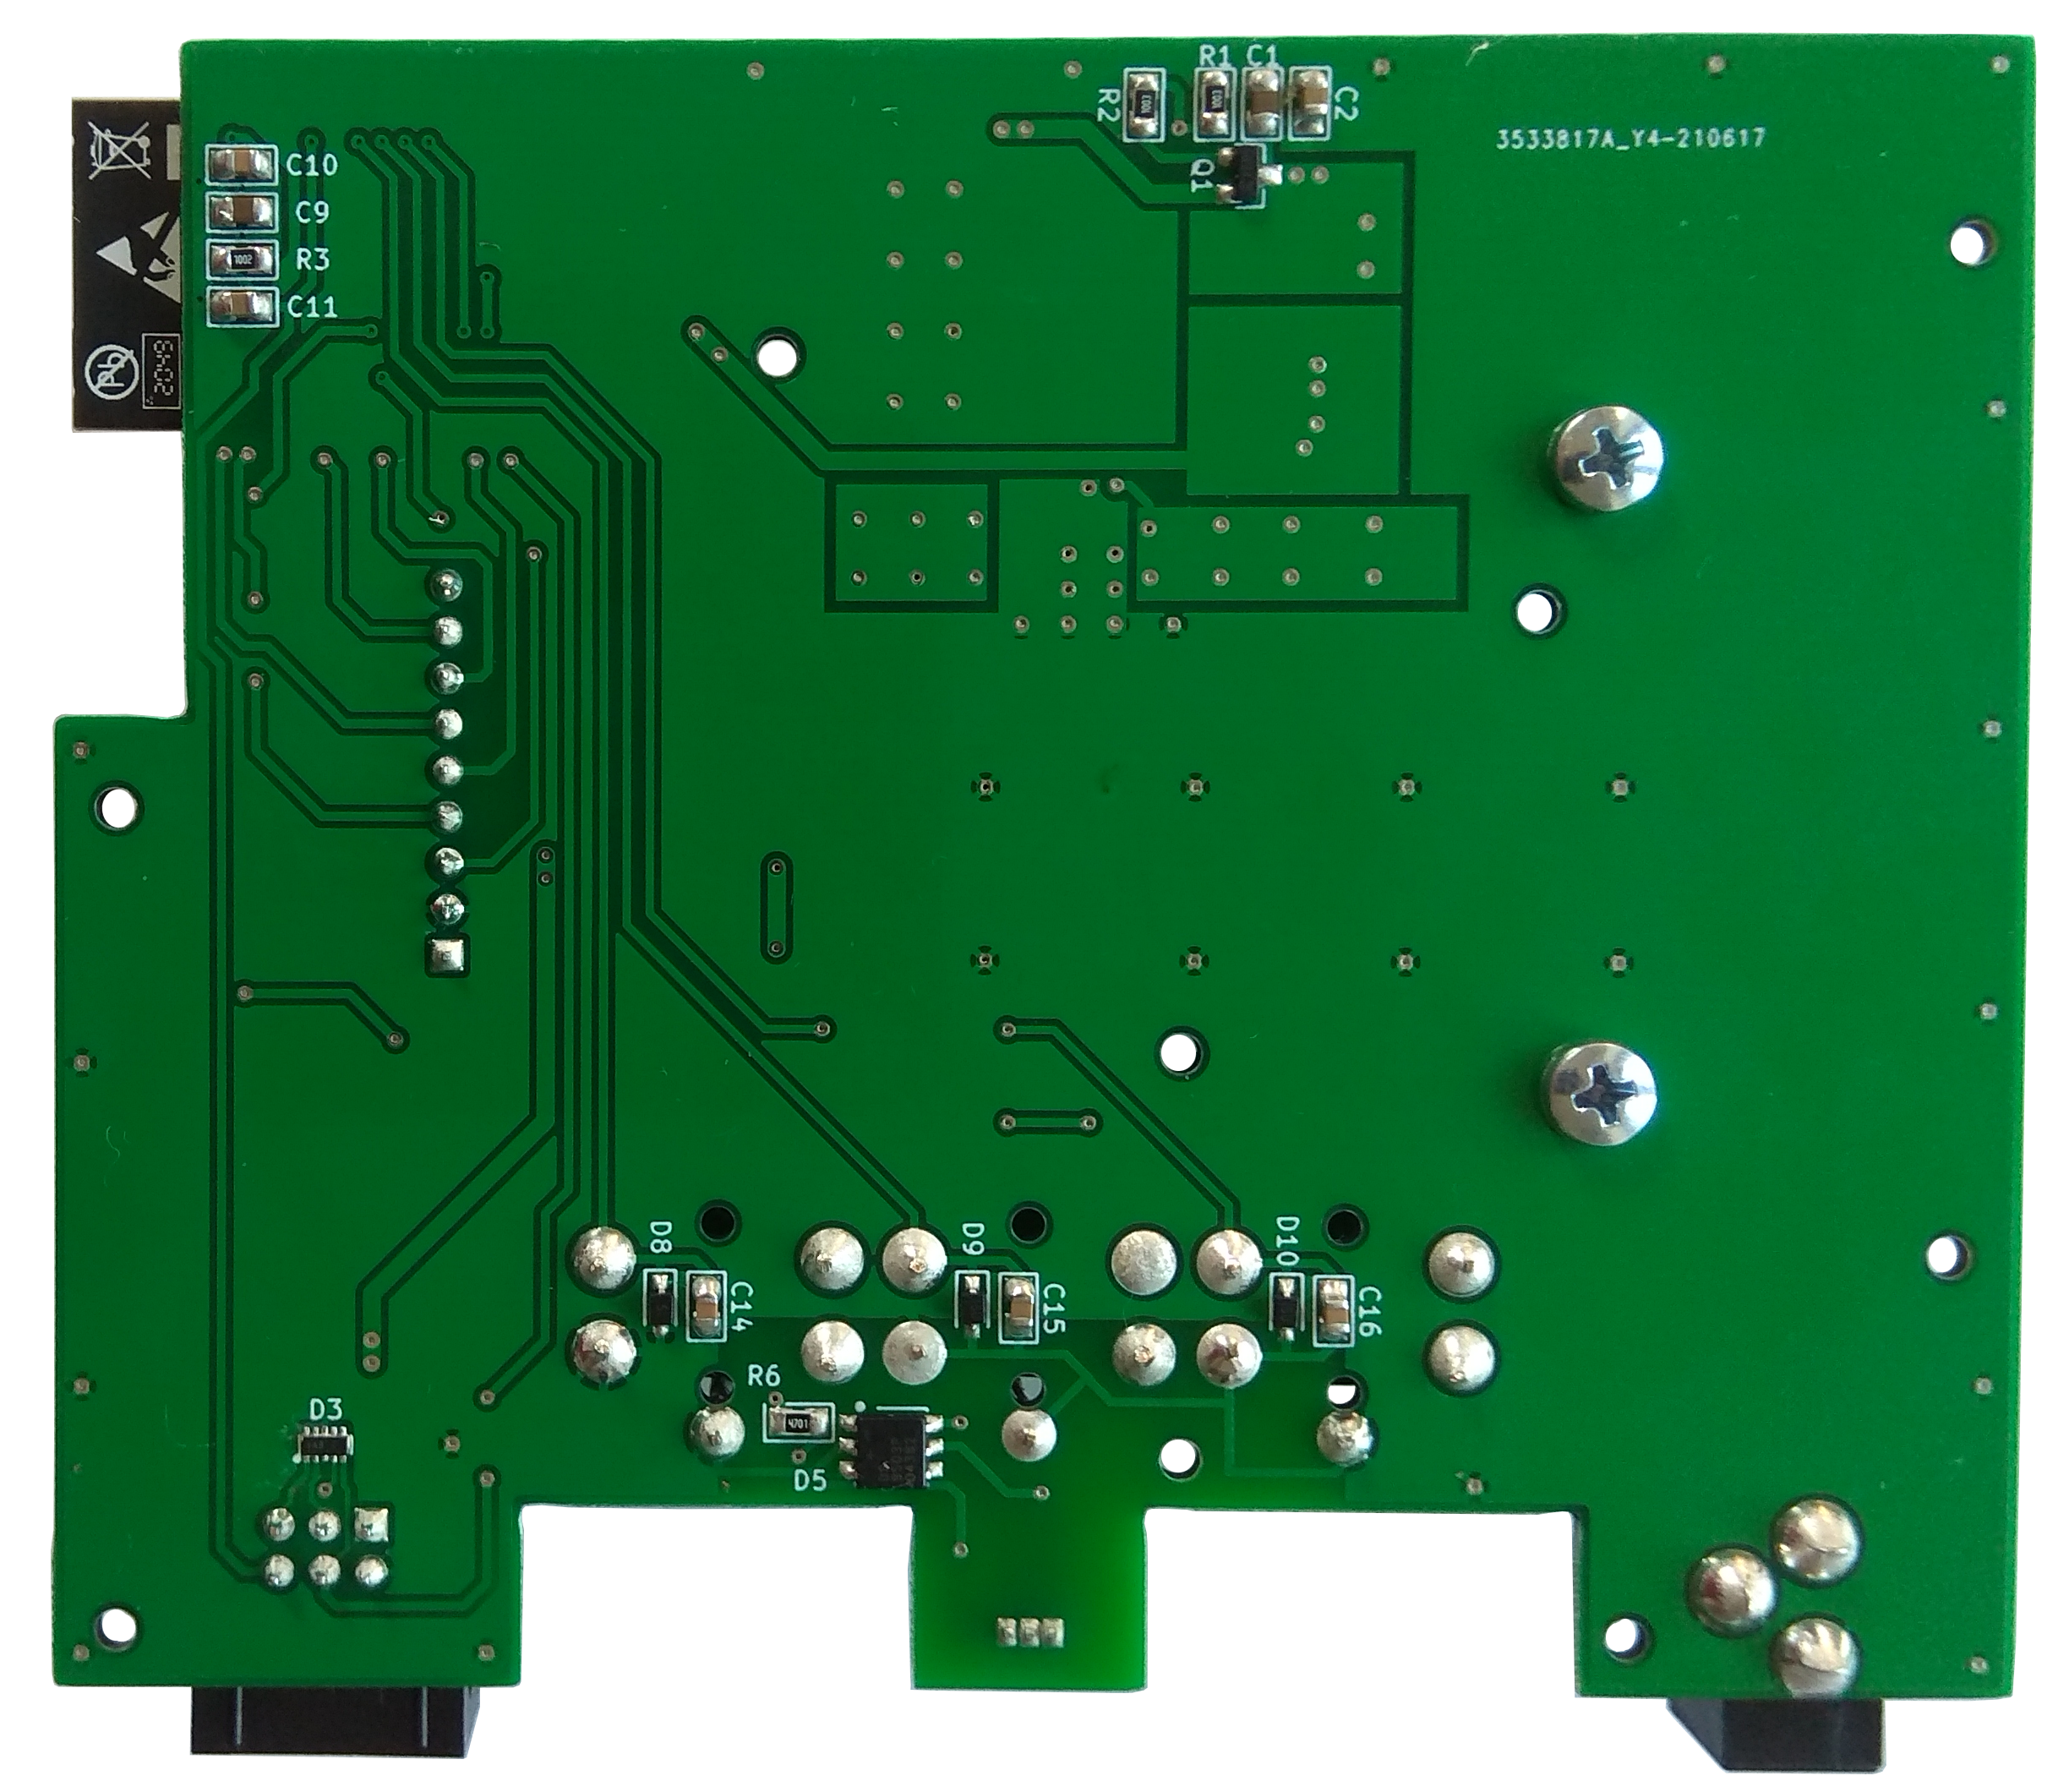
\includegraphics[width=\textwidth]{images/nastenny-snimac-prostorove-teploty-wifi/dps-nastenny-snimac-prostorove-teploty-wifi-spodni-cast.png}
    \caption{Spodní strana.}
    \label{fig:dps-nastenny-snimac-prostorove-teploty-wifi-spodni-cast}
\end{subfigure}
\caption{DPS nástěnného snímače prostorové teploty (verze WiFi).}
\label{fig:dps-nastenny-snimac-prostorove-teploty-wifi}
\end{figure}


\begin{figure}[H]
    \centering
    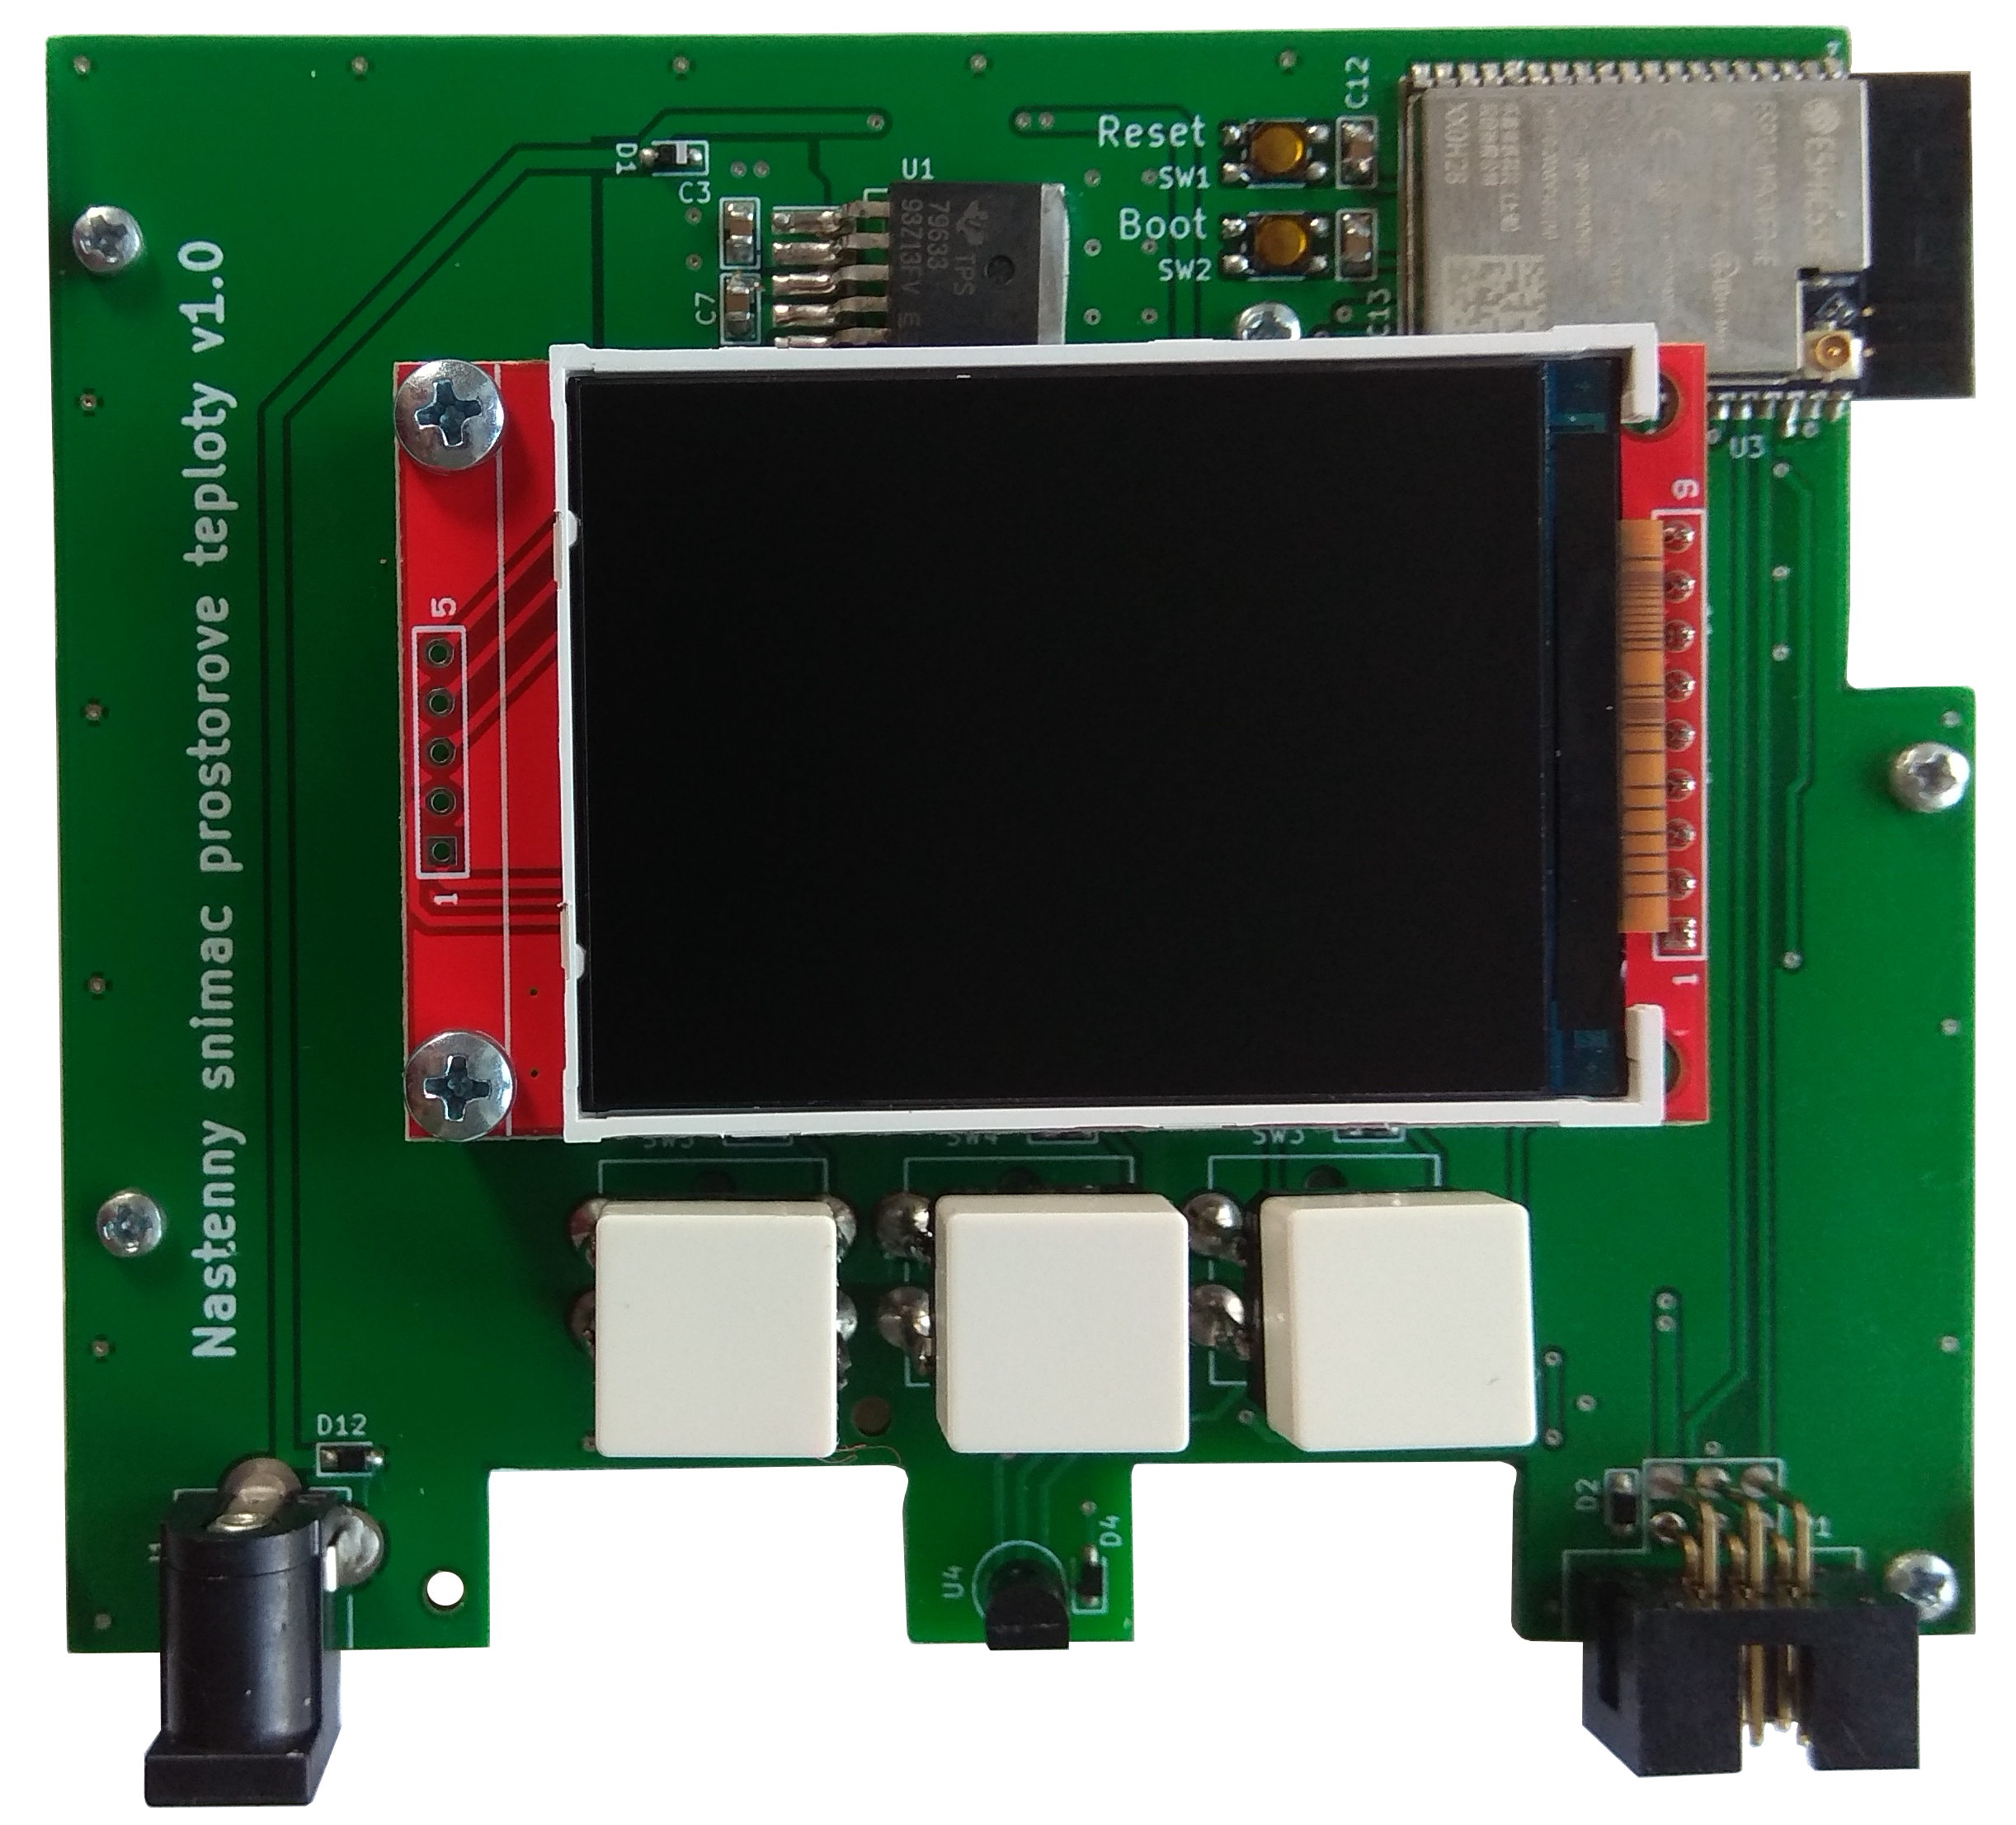
\includegraphics[width=0.85\textwidth]{images/nastenny-snimac-prostorove-teploty-wifi/dps-nastenny-snimac-prostorove-teploty-wifi-vrchni-cast-displej.png}
    \caption{DPS nástěnného snímače prostorové teploty (verze WiFi) s~displejem, vrchní strana.}
    \label{fig:dps-nastenny-snimac-prostorove-teploty-wifi-vrchni-cast-displej}
\end{figure}
\begin{figure}[H]
    \centering
    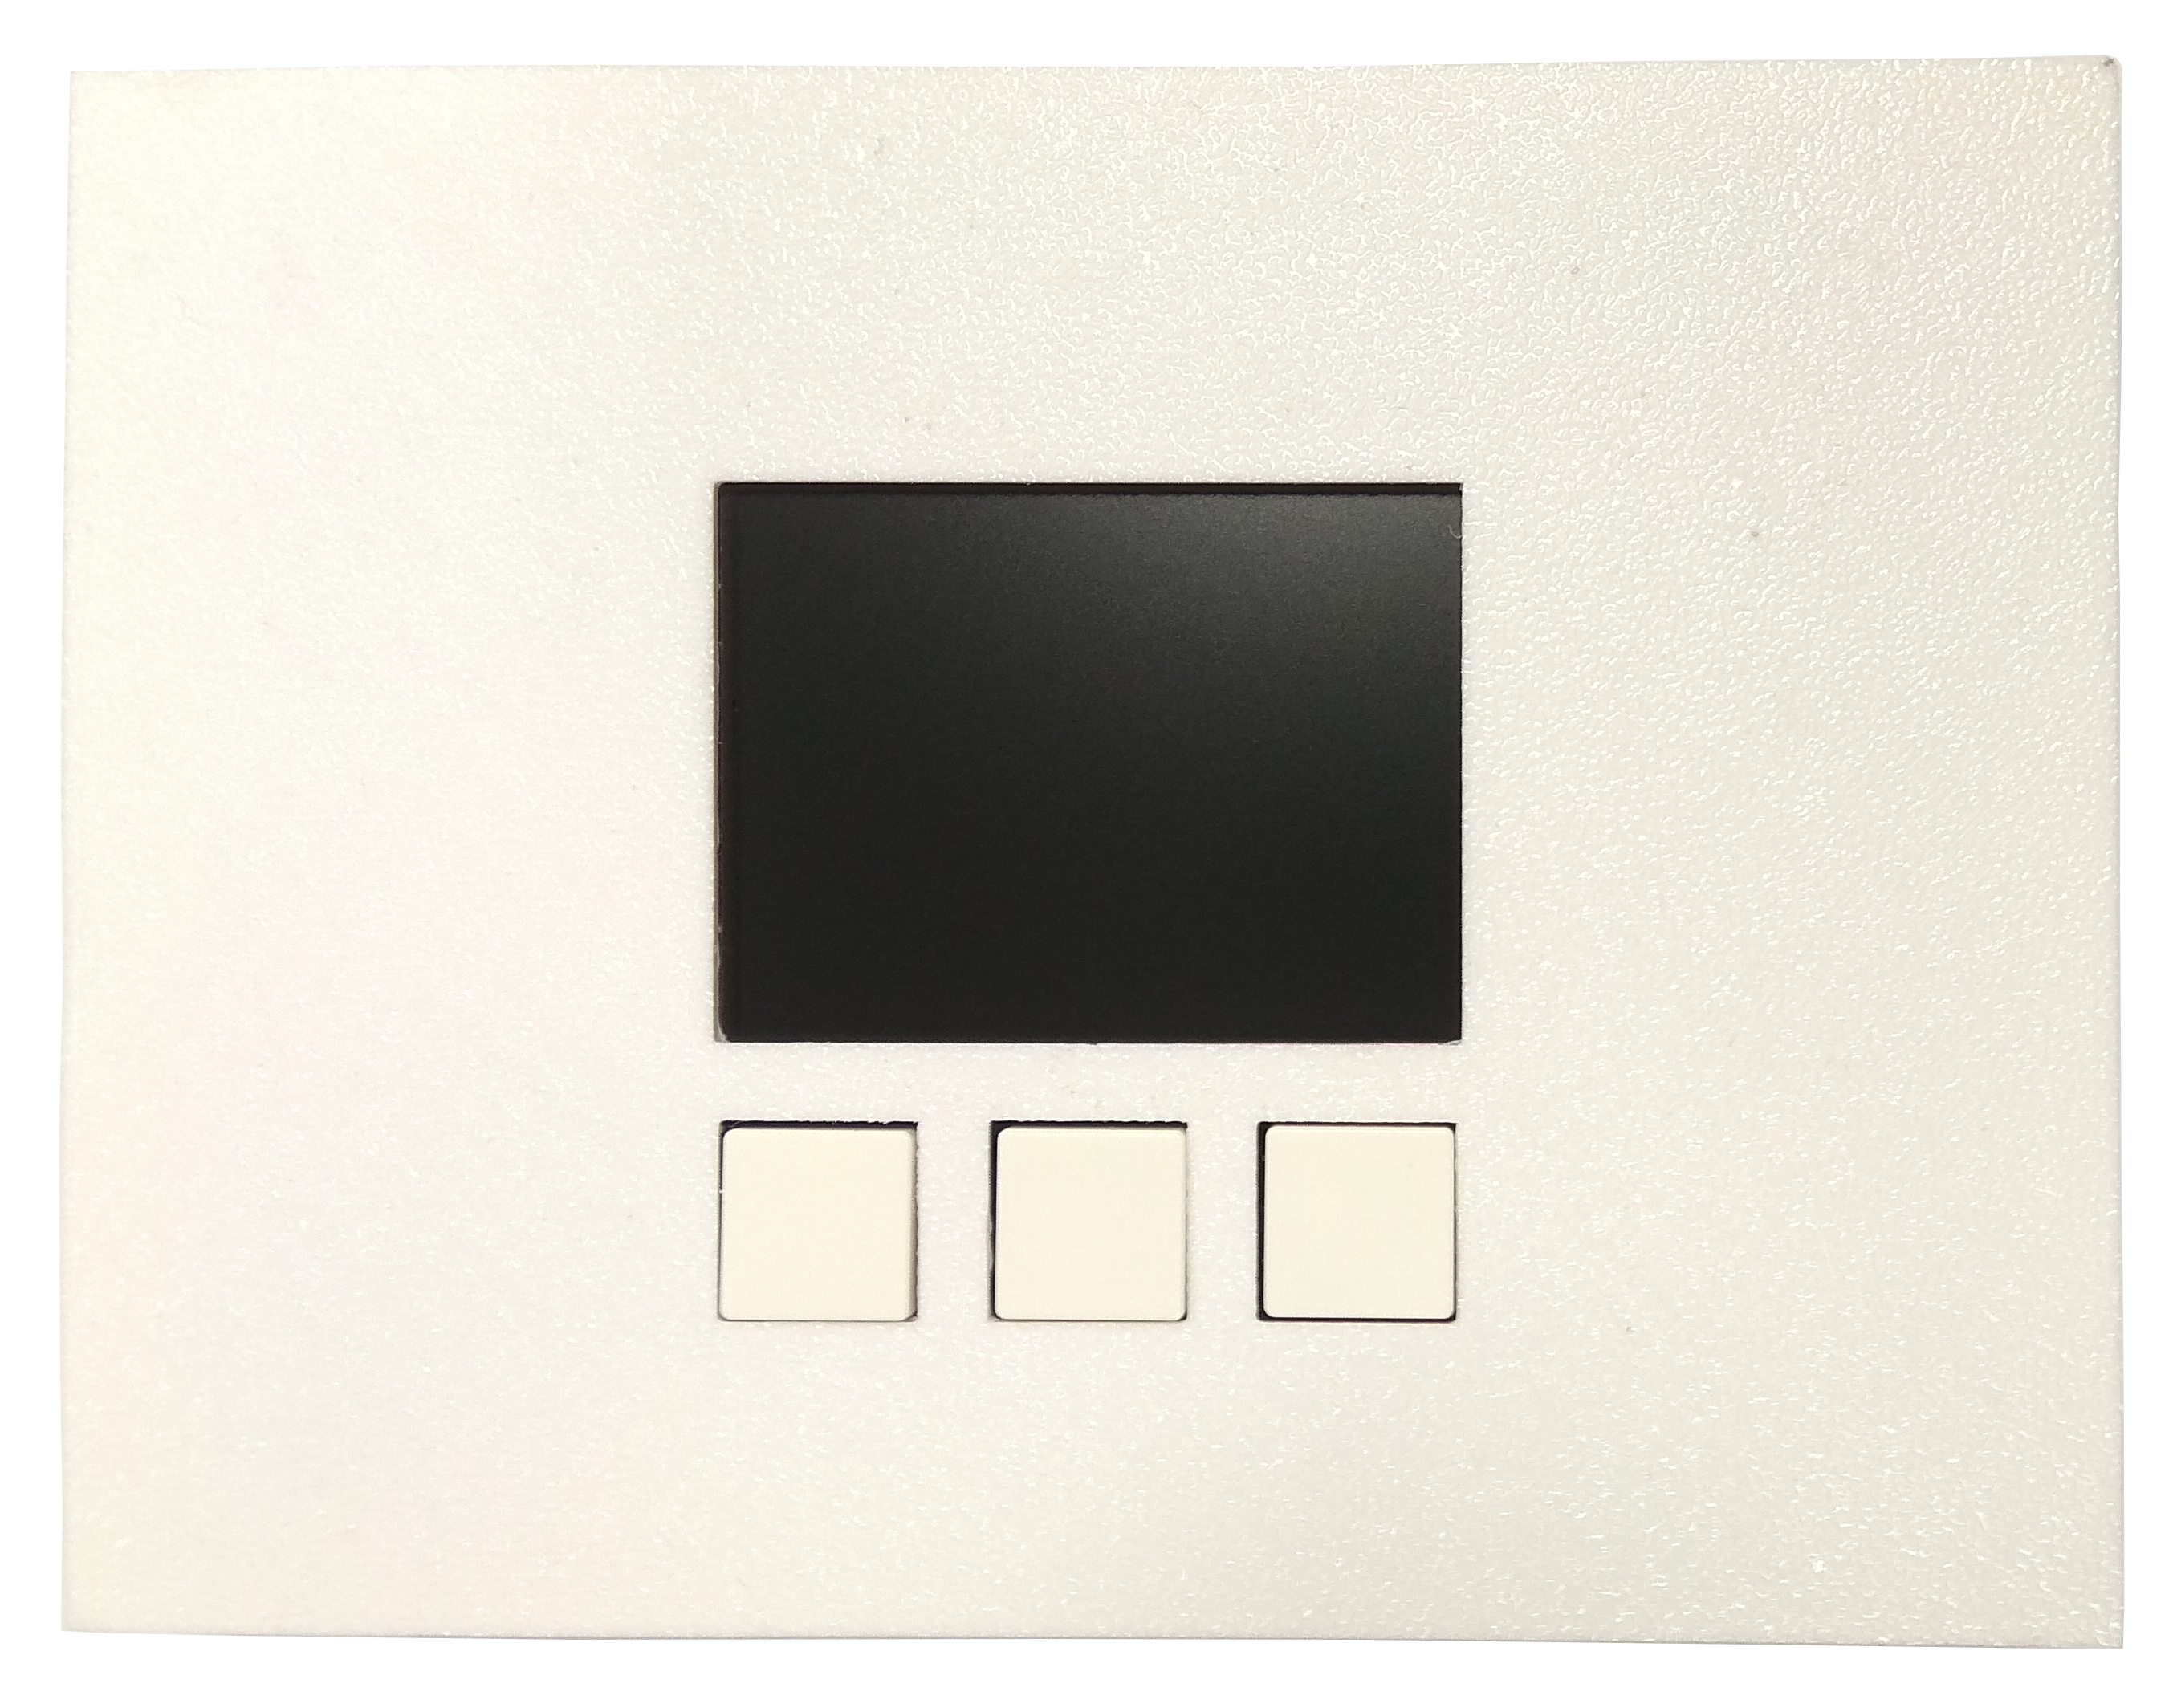
\includegraphics[width=\textwidth]{images/krabicka-nastenny-snimac-prostorove-teploty/krabicka-nastenny-snimac-prostorove-teploty-predni-strana.png}
    \caption{Přední část krabičky.}
    \label{fig:krabicka-nastenny-snimac-prostorove-teploty-predni-strana}
\end{figure}

\begin{figure}[H]
    \centering
    \includegraphics[width=\textwidth]{images/krabicka-nastenny-snimac-prostorove-teploty/krabicka-nastenny-snimac-prostorove-teploty-predni-strana-zezadu.png}
    \caption{Zadní strana přední části krabičky.}
    \label{fig:krabicka-nastenny-snimac-prostorove-teploty-predni-strana-zezadu}
\end{figure}

\begin{figure}[H]
    \centering
    \includegraphics[width=\textwidth]{images/krabicka-nastenny-snimac-prostorove-teploty/krabicka-nastenny-snimac-prostorove-teploty-spodni-cast.png}
    \caption{Spodní část krabičky.}
    \label{fig:krabicka-nastenny-snimac-prostorove-teploty-spodni-cast}
\end{figure}

\begin{figure}[H]
    \centering
    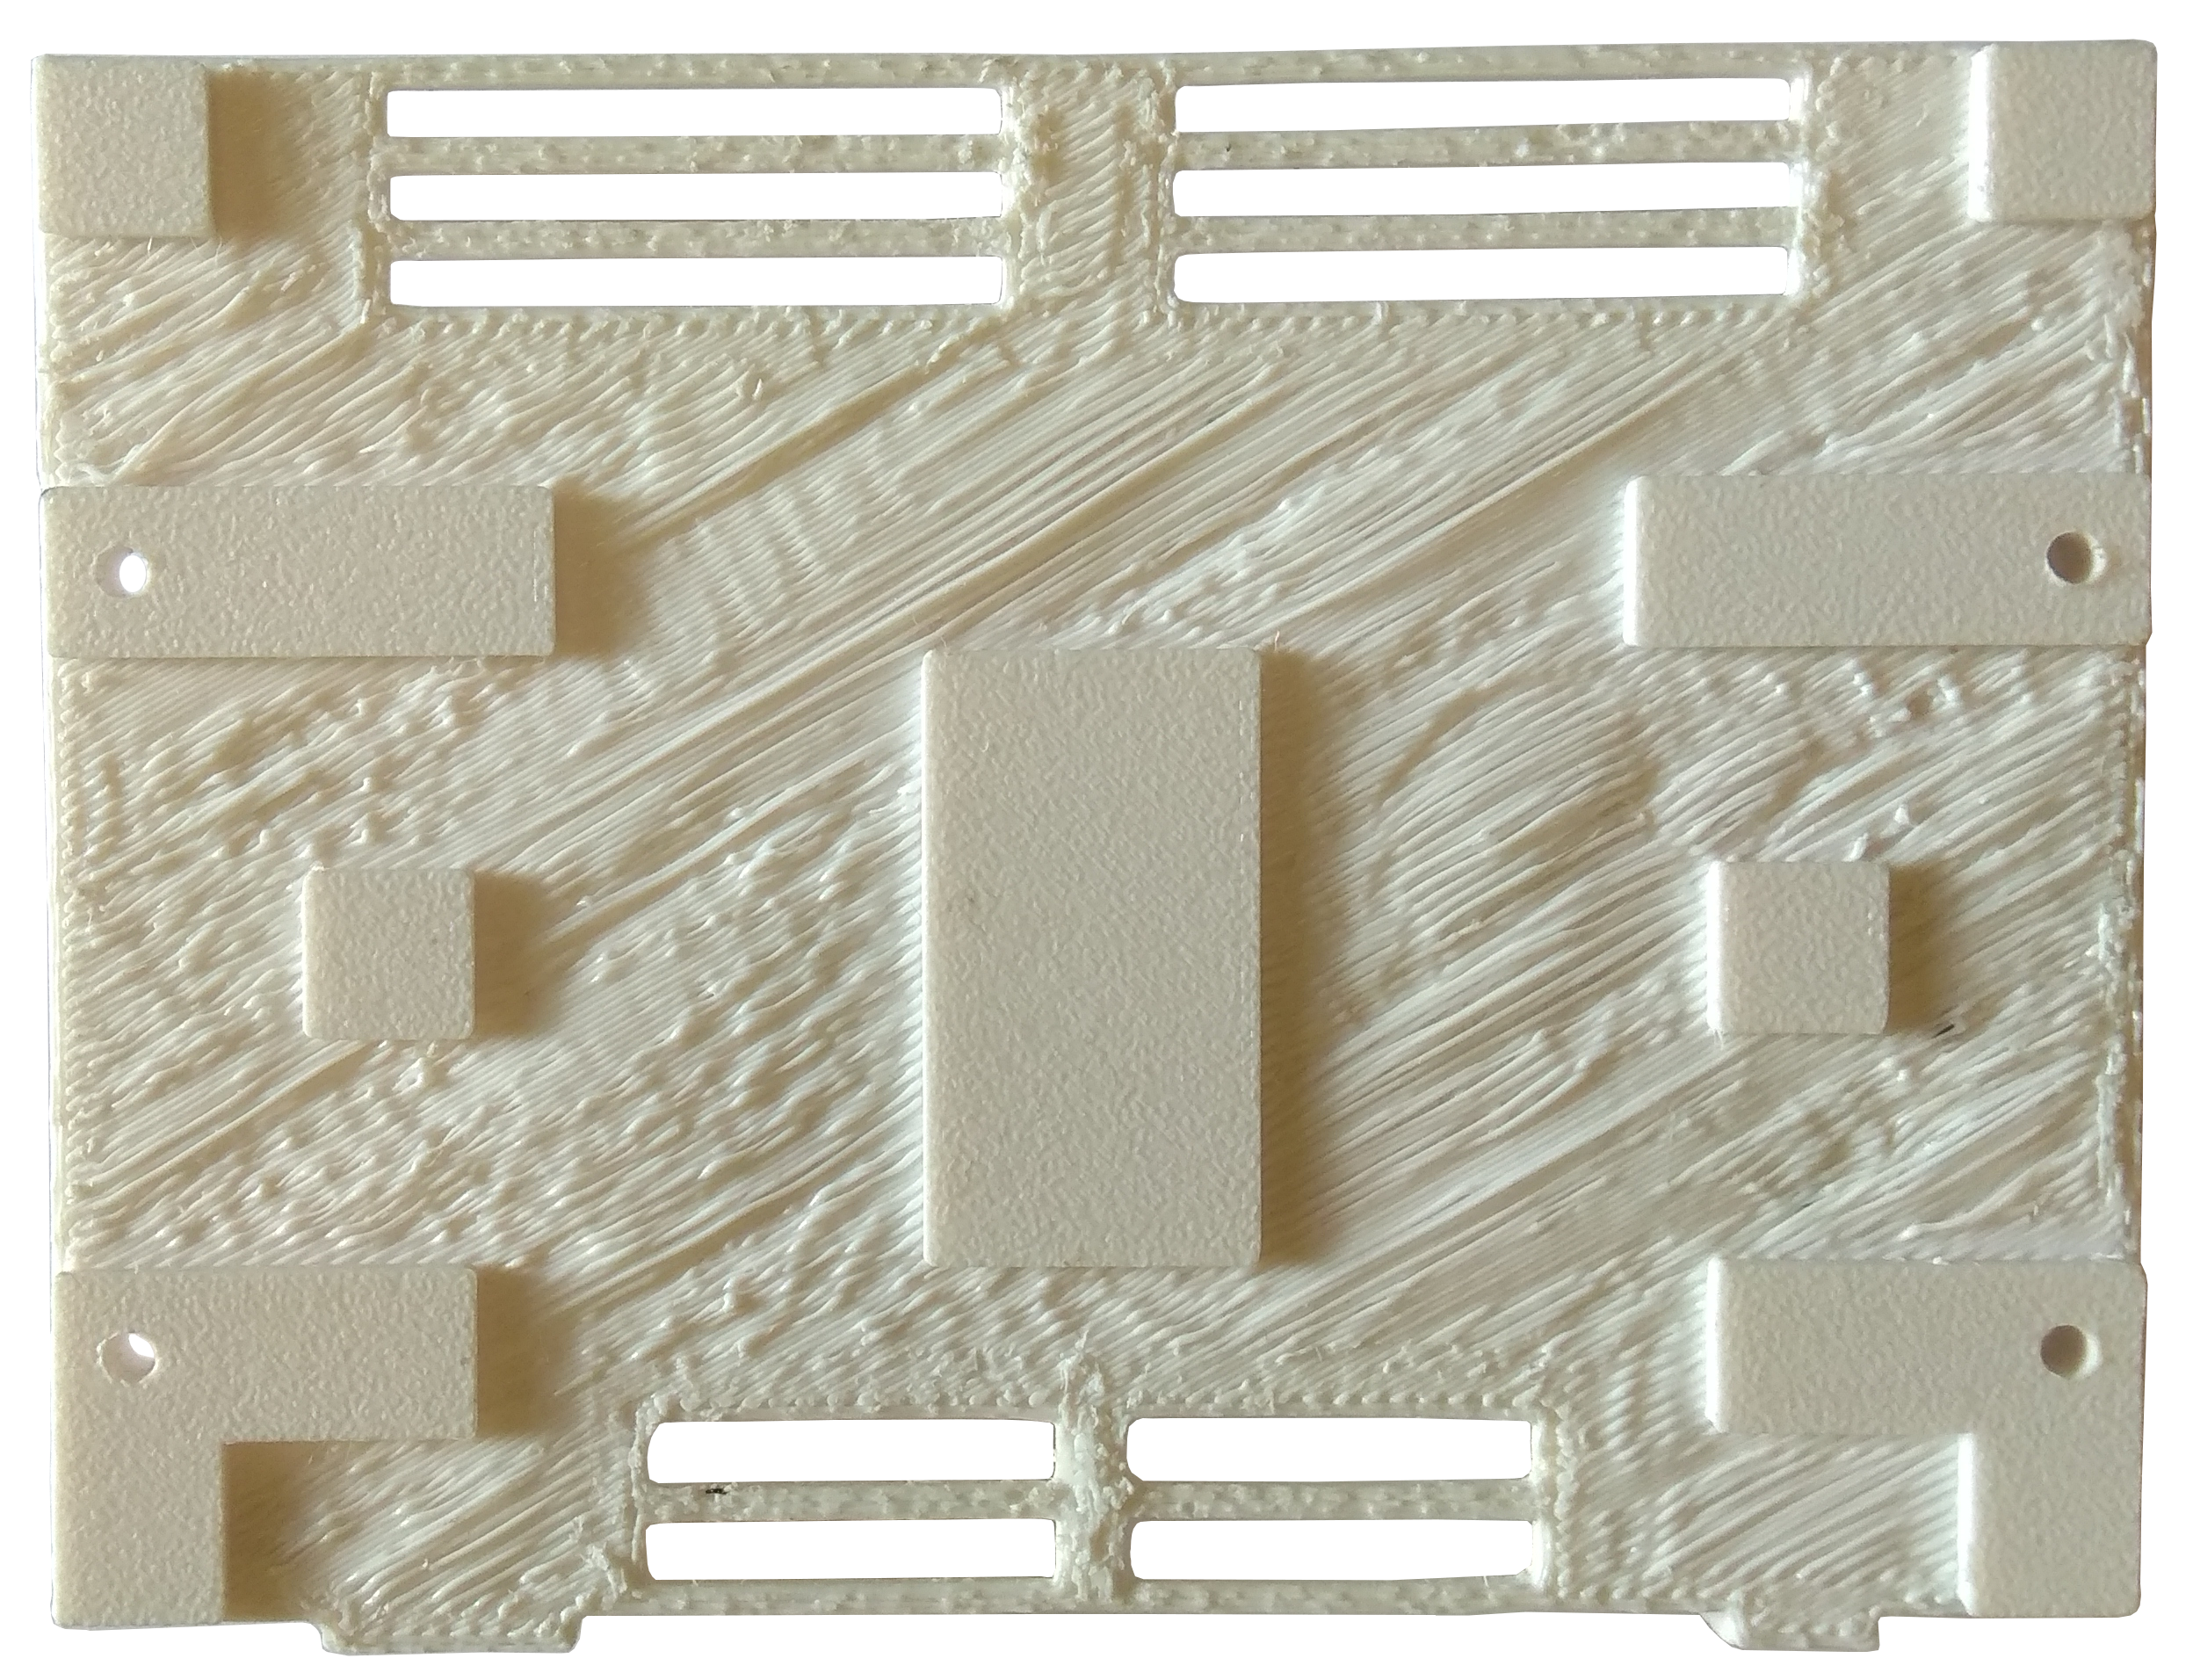
\includegraphics[width=\textwidth]{images/krabicka-nastenny-snimac-prostorove-teploty/krabicka-nastenny-snimac-prostorove-teploty-spodni-cast-zezadu.png}
    \caption{Zadní strana spodní části krabičky.}
    \label{fig:krabicka-nastenny-snimac-prostorove-teploty-spodni-cast-zezadu}
\end{figure}

\begin{figure}[H]
    \centering
    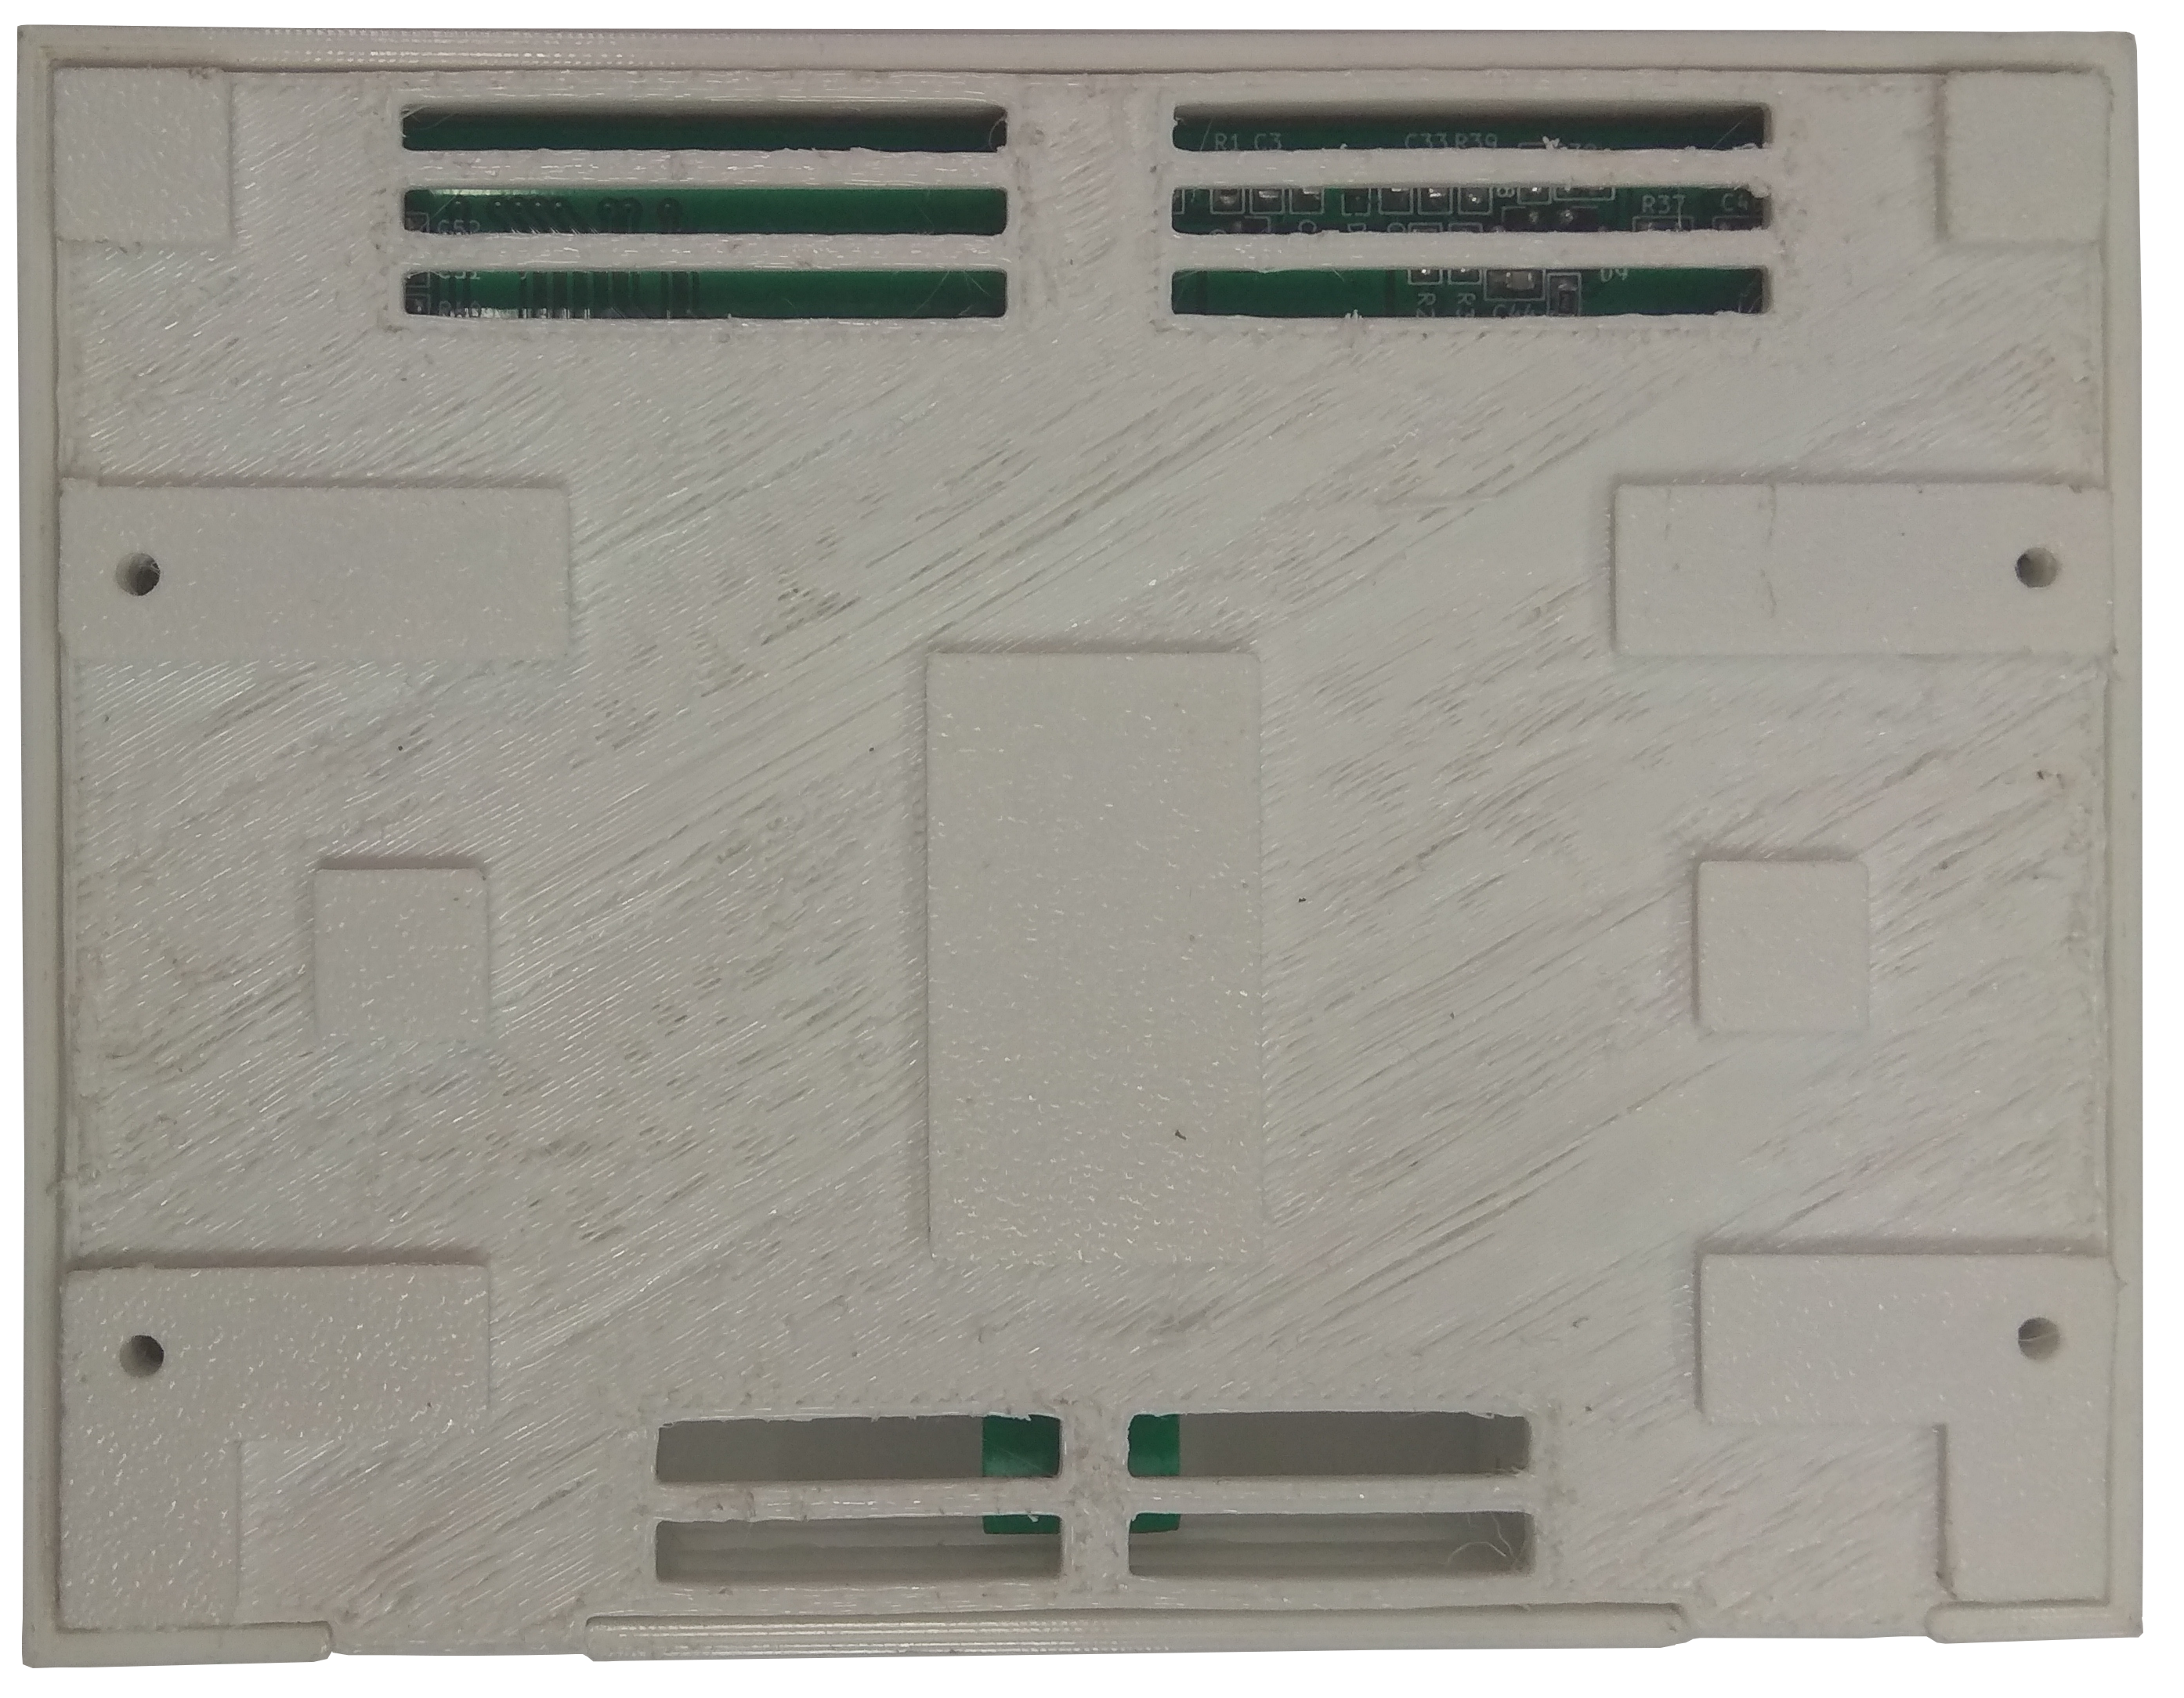
\includegraphics[width=\textwidth]{images/krabicka-nastenny-snimac-prostorove-teploty/krabicka-nastenny-snimac-prostorove-teploty-spodni-cast-zezadu-dps.png}
    \caption{Zadní strana spodní části krabičky s vloženou DPS.}
    \label{fig:krabicka-nastenny-snimac-prostorove-teploty-spodni-cast-zezadu-dps}
\end{figure}

\begin{figure}[H]
    \centering
    \includegraphics[width=\textwidth]{images/krabicka-nastenny-snimac-prostorove-teploty/krabicka-nastenny-snimac-prostorove-teploty-ethernet-celni-strana.png}
    \caption{Čelní strana krabičky, verze s Ethernetem.}
    \label{fig:krabicka-nastenny-snimac-prostorove-teploty-ethernet-spodni-cast-zezadu}
\end{figure}

\begin{figure}[H]
    \centering
    \includegraphics[width=\textwidth]{images/krabicka-nastenny-snimac-prostorove-teploty/krabicka-nastenny-snimac-prostorove-teploty-bocni-strana.png}
    \caption{Boční strana krabičky.}
    \label{fig:krabicka-nastenny-snimac-prostorove-teploty-prava-strana}
\end{figure}

\begin{figure}[H]
    \centering
    \includegraphics[width=\textwidth]{images/krabicka-nastenny-snimac-prostorove-teploty/krabicka-nastenny-snimac-prostorove-teploty-ethernet-spodni-cast-dps.png}
    \caption{Spodní část krabičky s osazenou DPS.}
    \label{fig:krabicka-nastenny-snimac-prostorove-teploty-ethernet-spodni-cast-dps}
\end{figure}

\begin{figure}[H]
    \centering
    \includegraphics[width=\textwidth]{images/krabicka-nastenny-snimac-prostorove-teploty/krabicka-nastenny-snimac-prostorove-teploty-ethernet-celni-strana-dps.png}
    \caption{Pohled na čelní stranu s osazenou DPS.}
    \label{fig:krabicka-nastenny-snimac-prostorove-teploty-ethernet-celni-strana-dps}
\end{figure}

\begin{figure}[H]
    \centering
    \includegraphics[width=\textwidth]{images/krabicka-nastenny-snimac-prostorove-teploty/krabicka-nastenny-snimac-prostorove-teploty-bocni-strana-dps.png}
    \caption{Boční strana s osazenou DPS.}
    \label{fig:krabicka-nastenny-snimac-prostorove-teploty-bocni-strana-dps}
\end{figure}
\section{Převodník USB-UART CP2102N}
\label{sec:prevodnik-usb-uart-cp2102n}
Pro programování nástěnného snímače prostorové teploty, přesněji modulu ESP32 Wrover-IE je použit převodní USB-UART CP2102N od firmy Silocon Labs. Zakoupil jsem již hotový modul CP2102N MINEK (obrázek \ref{fig:prevodnik-cp2102n-modul-vrchni-cast}). Modul je doplněn o zapojení tranzistoru pro automatický reset a automatický boot modulu (obrázek \ref{fig:prevodnik-cp2102n-modul-spodni-cast}). Z modulu se využívají signály \acrshort{dtr} (\textit{\acrlong{dtr}}) a \acrshort{rts} (\textit{\acrlong{rts}}). Pokud je potřeba vstoupit do bootloaderu pro nahrání nového firmwaru, je nutné podržet boot a~následně stisknout reset, zařízení je tak připraveno nahrát nový firmware. V případě využití signálu DTR a RTS se tato operace dělá automaticky, nicméně z~pravdivostní tabulky \ref{tab:pravdivostni-tabulka-pro-automaticky-boot} není vidět stav pro EN = 0, IO0 = 0, tento stav je zajištěn pomocí kondenzátoru o velikosti 1\textmu  F mezi EN vstup a~GND. Tímto kondenzátorem se zajistí zpoždění při přechodu z log. 0 na log. 1 na vstupu EN, zároveň v~tomto zpoždění je vstup IO0 v log. 0 a je možné vstoupit do bootloaderu. Z modulu jsou do konektoru vyvedeny 5 V, GND, RXD, TXD, EN a IO0. Komunikace mezi CP2102N a modulem ESP32 pak probíhá po vodičích RXD a TXD. Schéma zapojení pro automatický bootloader s~využitím modulu CP2102N MINEK je v příloze \ref{app:schemata-ostatni}.

\begin{center}
\begin{table}[H]
\begin{tabular}{ |c|c||c|c| }  
 \hline
 \thead{DTR} & \thead{RTS} & \thead{EN} & \thead{IO0}\\
 \hline
 1 & 1 & 1 & 1 \\ 
 0 & 0 & 1 & 1 \\ 
 1 & 0 & 0 & 1 \\ 
 0 & 1 & 1 & 0 \\ 
 \hline
\end{tabular}
 \caption{Pravdivostní tabulka pro automatický boot modulu ESP32.}
 \label{tab:pravdivostni-tabulka-pro-automaticky-boot}
\end{table}
\end{center}


%\begin{figure}[H]
%    \centering
%    \includegraphics[width=0.5\textwidth]{images/prevodnik-usb-uart-cp2102n/prevodnik-cp2102n-modul-vrchni-cast.png}
%    \caption[Vrchní část modulu převodníku USB-UART.]{Vrchní část modulu převodníku USB-UART CP2102N MINEK s~výstupním konektorem pro programování zařízení.}
%    \label{fig:prevodnik-cp2102n-modul-vrchni-cast}
%\end{figure}


%\begin{figure}[H]
%    \centering
%    \includegraphics[width=0.5\textwidth]{images/prevodnik-usb-uart-cp2102n/prevodnik-cp2102n-modul-spodni-cast.png}
%    \caption[Spodní část modulu převodníku USB-UART.]{Spodní část modulu převodníku USB-UART s doplněnými tranzistory pro signály DTR a RTS pro automatický bootloader.}
%    \label{fig:prevodnik-cp2102n-modul-spodni-cast}
%\end{figure}



\begin{figure}[H]
\centering
\begin{subfigure}{.5\textwidth}
    \centering
    \includegraphics[width=\textwidth]{images/prevodnik-usb-uart-cp2102n/prevodnik-cp2102n-modul-vrchni-cast.png}
    \caption[Vrchní část modulu převodníku USB-UART.]{Vrchní část modulu převodníku USB-UART CP2102N MINEK s~výstupním konektorem pro programování zařízení.}
    \label{fig:prevodnik-cp2102n-modul-vrchni-cast}
\end{subfigure}%
\begin{subfigure}{.5\textwidth}
    \centering
    \includegraphics[width=\textwidth]{images/prevodnik-usb-uart-cp2102n/prevodnik-cp2102n-modul-spodni-cast.png}
    \caption[Spodní část modulu převodníku USB-UART.]{Spodní část modulu převodníku USB-UART s~doplněnými tranzistory pro signály DTR a RTS pro automatický bootloader.}
    \label{fig:prevodnik-cp2102n-modul-spodni-cast}
\end{subfigure}
\caption{Převodníku USB-UART CP2102N MINEK.}
\label{fig:prevodnik-cp2102n}
\end{figure}




\section{Softwarová část}

\subsection{Typy řízení vytápění}
V rámci řídicího systému existují tyto typy řízení:

\begin{itemize}
  \item Řízení vytápění podle chodbových termostatů.
  \item Řízení vytápění podle nástěnných snímačů prostorových teplot.
  \item Řízení vytápění podle teplotních plánů.
  \item Řízení vytápění podle teplotních plánů s úpravou podle předpovědi počasí.
\end{itemize}

Předpokládá se, že centrální zásobník otopné vody je průběžně ohříván během dne pomocí přebytků energie přes výměníky u krb. Tím se tedy předpokládá, že zásobník je nahřán pro případné potřeby vytápění. Je kladena priorita na získávání ohřáté otopné vody ze zdroje tepla zmíněná dříve. Uživatelé jsou upozorňováni signalizací na displejích jak u krbů, tak i na nástěnných snímačích prostorové teploty, přímo v řídícím systému (možné i notifikace na mobil, e-mail) či LED diodami (rozsvícení všech) u krbů, že je potřeba zatopit v krbech, pokud systém vyhodnotí, že je potřeb vytápět. V případě, že tomu k tomu nedojde využívá se plynový kondenzační kotel, který dohřívá zásobník (ten je možný ovládat automaticky).

V části \textbf{přehled} je pro přehlednost jsou jednotlivé teploty zobrazeny v části „jednotlivé teploty“, jsou zde všechny teploty snímané v zásobníku otopné vody, teploty na kouřovodech v přízemí a patře, v neposlední řadě jez zde i venkovní teplota. V části „porovnání teploty“ jsou zmíněné teploty zobrazeny v jednom grafu.

V části \textbf{nastavení} je možné v \textit{řízení teploty} vybrat jeden typ řízení vytápění (viz výše). Dále v \textit{módy řízení} je výběr módů a to zimní, letní nebo výběr podle venkovní teploty. Výběr módu má vliv na výběr mezních teplot pro spínání plynového kondenzačního kotle. Dané teplotní meze se dají nastavit v~části \textit{spínání plynového kotle} (teplotní meze pro léto a zimu). Tyto nastavené meze se berou pro kontrolu s teplotou v horní části zásobníku otopné vody. Pokud teplota v~horní části zásobníku je menší než teplota definovaná v části „min. zapnutí“ dojde k zapnutí kotle pro nahřátí otopné vody, kotel se vypíná při teplota definované v části „max. vypnutí“. Při porovnávání teplot se též bere v potaz nastavená hystereze v části \textit{ostatní nastavení}. Při výběru módu podle venkovní teploty dochází k automatickému výběru letního nebo zimního módu. Teplotní mez pro výběr letního módu (v rámci módu podle venkovní teploty) je definovaná v části „min. venkovní teplota pro letní mód“. Toto spínání kotle nastává v momentě, kdy po upozornění uživatelů nedojde k zatopení v krbech.

V části nastavení \textit{krby – spínání čerpadel} se definují minimální hranice teploty, kdy dojde k sepnutí oběhových čerpadel pro krbové výměníky, tedy při jaké teplotě se má brát v potaz, zda někdo v krbu zatopit a mají se spustit čerpadla pro nahřívání zásobníku otopné vody. Toto nastavení je poměrně důležité a kontrola těchto teplot je zcela nezávislá na dalších nastaveních (automatizaci) v systému, je potřeba vždy při zatopení spustit čerpadla, jinak dojde k přehřátí vody ve výměníku krbu. V případě přehřátí se aktivuje ochrana přímo u krbů a dojde k ke zvukové signalizaci přehřátí, pokud teplota neklesne za určitou dobu, dojde k aktivování ochranných ventilů a vypuštění přehřáté vody.


V části \textit{LED indikace – mezní parametry zásobníku otopné vody} se definují mezní teploty pro horní, střední a spodní část zásobníku otopné vody. Tato signalizace se zejména týká pro krby, aby uživatel věděl, zda může topit a jak je moc zásobník nahřátý. U modré LED se definuje mezní minimální teplota, kterou by zásobníku ve horní části měl mít (povolení pro topení). U oranžové LED se definuje mezní maximální teplota, kdy ve střední části zásobníku dochází k dostatečnému nahřátí otopné vody (oznámení, že za chvilku by se mělo přestat topit). U červené LED se definuje mezní maximální teplota, kdy ve spodní části zásobníku je plně ohřátá(okamžitě přestat topit.). Aktivace červené LED předchází v dostatečném předstihu před aktivováním ochrany u~krbů pro přehřátí otopné vody, popsáno v předchozím odstavci.
\subsubsection{Řízení vytápění podle chodbových termostatů}
V přízemí a v patře je na chodbě umístěn jeden lokání termostat popsaný v části \ref{sec:digitalni-chodbove-termostaty}. Tento termostat na základě lokálního nastavení (není součástí řídicího systému) spínání/rozpínání výstupní relé při požadavku na vytápění. Tento požadavek se následně vyhodnotí v centrálním systému a dojde k sepnutí nebo rozepnutí daného chodbového oběhového čerpadlo pro podlahové vytápění a otevření všech okruhů podlahové vytápění. Dochází tedy k řízení vytápění všech místností na patře podle jednoho centrálního termostatu. 

\subsection{Záložka zařízení}
V části „koncová zařízení“ se zobrazují jednotlivá ovládána (zapnuto/vypnuto) zařízení otopné soustavy, tedy plynový kondenzační kotel, čerpadla pro krby s výměníkem, čerpadla pro podlahové vytápění a zapnutí signalizačních LED u krbů. Je možné samotnou automatizaci respektive ovládání zmíněných zařízení řídit podle vlastního uvážení, proto slouží přepínač „manuální ovládání zařízení“, zde si pak uživatel může libovolně jednotlivá zařízení ovládat bez ohledu na nastavenou automatizaci.

V části „termostaty chodby – požadavek topení“, zde se zobrazuje zda dochází k vytápění v přízemí či patře na základě nastavení lokálních termostatů na chodbách.

V části „ovládání čerpadel – vodní kámen“ slouží ke spínání čerpadel pro ochranu před zatuhnutím lopatek. Vzhledem k místní dosti tvrdé vodě, došlo při netopení v přízemí, tedy při nevyužívání daných čerpadel k zatuhnutí lopatek v důsledku nánosu vodního kamene. Pro se zde nachází nastavení, kde si uživatel může pro konkrétní den, hodinu a definovanou délku nastavit spínání čerpadel pro odstranění nánosu na lopatách. Ideální volbou je otopnou vodu zbavit minerálů nebo vyměnit za destilovanou vodu, nicméně k některým méně kvalitnějším provedením spojům trubek otopné soustavy, by docházelo k průsaku otopné vody. Proto je otopná vody z řádu s vyšším podílem minerálů jedním z řešení, jak docílit zaslepení průsaku především vápníkem bez nutnosti, alespoň prozatím, spoje opravovat.

Výše popsané části jsou zobrazená na obrázku \ref{fig:ha-zarizeni}.




\begin{figure}[H]
    \centering
    \includegraphics[width=0.90\textwidth]{images/software-ha/ha-zarizeni.png}
    \caption{Záložka zařízení v HA.}
    \label{fig:ha-zarizeni}
\end{figure}

\subsection{Vývoj pro zónovou regulaci}

Na obrázku \ref{fig:teplotni-plan} je zobrazen možný nastavitelný teplotní plán pro celý den. Lze tak nastavit všechny dny v týdnu. Pro každý zvolený teplotní úsek je možné si zvolit požadovanou teplotu.

\begin{figure}[H]
    \centering
    \includegraphics[width=0.90\textwidth]{images/software-ha/teplotni-plan.png}
    \caption{Nastavitelný teplotní plán pro danou hodinu v celém dni.}
    \label{fig:teplotni-plan}
\end{figure}

Na obrázku \ref{fig:termostat-v-mistnosti} je nastavení aktuální teploty pro požadovanou místnost. Každá místnost má svoje vlastní nastavení. Zobrazuje se zde aktuálně naměřená teplota v dané místnosti a požadovaná teplota. Pokud dojde k~přenastavení požadované teploty, dojde k přenesení této teploty do nástěnného snímače prostorové teploty, přenos funguje i opačně.

\begin{figure}[H]
    \centering
    \includegraphics[width=0.90\textwidth]{images/software-ha/termostat-v-mistnosti.png}
    \caption{Zobrazení aktuální teploty z dané místnosti, možnost nastavit požadovanou teplotu.}
    \label{fig:termostat-v-mistnosti}
\end{figure}




\chapter{Testování}
\subsection{Naměřená data pro řízení podle teplotních plánů}
\subsection{Naměřená data pro řízení podle teplotních plánů s úpravou předpovědi počasí}

\chapter{Návrh dalšího vylepšení}
Vzhledem k používání rekuperace v domě. Rozvést kabely s teplotními senzory do jednotlivých průduchů ve stropě. Snímat výstupní teplotu, která je ochlazena z venkovního prostředí a tuto sníženou teplotu kompenzovat zapnutím vytápění, aby nedocházelo k poklesu teploty v místnosti, respektive její minimalizace.

V budoucnu se počítá s pořízením solárních panelů. Primárním cíle bude ohřívat otopnou vodu v centrálním zásobníku. Přebytky energie ukládat do akumulátorů. Využít stávající systém pro přepínání kam danou energii využít, měřit získanou a spotřebovanou energii.

Doplnit záložní akumulátory v případě výpadku elektrické energie. Zejména pro čerpadla u krbů pro odvedení ohřáté vody z krbového výměníku. V~současné době krby disponují ochranou proti přehřátí spočívající v ochranném ventilu.

V rámci centrálního systému doplnit možnost kopírování teplotních plánů a usnadnit tak jejich tvorbu. 



%\blindmathtrue

%\blinddocument

\chapter{Závěr}
Podle zadání diplomové práce se mi povedly splnit všechny body. Cílem práce bylo prostudovat problematiku zónového podlahového vytápění a navrhnout vlastní řešení pro řízení dílčích částí systému. Navrhl jsem koncept centrální jednotky a dalších částí pro zónovou regulaci vytápění. Navrhl jsem koncept komunikace centrální jednotky, lokálních \acrshort{nspt} a~akčních členů pro řízení jednotlivých otopných okruhů. Na základě konceptu jsem zvolil centrální jednotku, navrhl jednotlivá zařízení pro dané části systému, včetně jejich mechanického umístění a ochranných krabiček. Některé části jsem zakoupil hotové a~případně je upravil. V~rámci problematiky POE jsem navrhl DC/DC měnič pro PSE zařízení. Dalším splněným bodem zadání je zvolená vhodná komunikace a zejména jednoduchá rozšiřitelnost. Na centrální jednotce funguje open-source řídicí systém pro domácí automatizaci. Tento systém je neustále rozšiřován a aktualizován vývojářskou komunitou. Má již mnoho integrovaných částí pro řízení vytápění. V~rámci komunikace mezi centrální jednotkou a~\acrshort{nspt} byla zvolena komunikace pomocí MQTT, která je snadno nastavitelná a snadno rozšiřitelná. Mezi centrální jednotkou a akčními členy se využívá standardní I$^2$C sběrnice s úpravou pro komunikaci na delší vzdálenosti. Teplotní senzory jsou připojené na 1-Wire sběrnici. Zhotovil jsem \acrshort{nspt} do jednotlivých místností ve verzi s POE a WiFi s napájením pomocí síťového adaptéru. Pro \acrshort{nspt} jsem navrhl a~zhotovil krabičku pomocí 3D tiskárny. Pro ovládání jednotlivých otopných okruhů jsem zhotovil vlastní řešení s využitím zakoupených termoelektrických pohonů. V rámci celého systému se využívá automatizovaná část (inteligentní část) spočívající využívání teplotních plánů s možností jejich modifikování na základě teplotní predikce, kterou jsem do systému implementoval. Využívají se nasbíraná data z~jednotlivých místností v~rámci vytápění a~na základě nich se sestavuje velmi jednoduchá lineární predikci s předpovědí počasí pro úpravu časových teplotních úseků, aby v~požadovaný čas bylo dosaženo požadované teploty. Dále se využívá softwarová detekce otevřeného okna pro pozastavení vytápění v případě otevření okna. Vše jsem následně otestoval a nasadil v rodinném domě. Systém se dá neustále rozšiřovat pro případné požadované úpravy. Vše tak bylo upravováno podle požadavků uživatelů domácnosti. 

Celý systém řízení se postupně vyvíjel. Původně bylo řízení vytápění podle chodbových termostatů a nepočítalo se se zónovým řízením podlahového vytápění na které se následně přešlo. Majitel domu chtěl primárně veškeré řešení drátové. Proto se nakonec vymýšlelo, jak rozvést kabely do jednotlivých místností. Vznikly primárně POE \acrshort{nspt}, využilo se půdy pro rozvedení UTP kabelu do všech místností, kde to bylo možné a~zároveň nebyla ničena estetika místnosti. Pro místnosti, kde to nebylo možné, jsem navrhl bezdrátové moduly (WiFi) s~napájením ze síťových adaptérů, aby nebylo nutné se starat o výměnu baterií, požadavek majitele. Jistou nevýhodou mohou být bezdrátové moduly z~pohledu bezdrátové komunikace a případných výpadků. Vzhledem k dobrému pokrytí WiFi sítě v~domě je komunikace bezproblémová. Celkové náklady na celý systém jsou po zaokrouhlení 35 700 Kč. Nezanedbatelnou část částky tvoří termoelektrické pohony (celkově 2 × 12 pohonů pro 1. a 2. druhé patro), která činí přibližně 10 000 Kč. Cenové srovnání s~komerčními systému nedává úplně smysl. V mé cenové kalkulaci nejsou zahrnuté náklady například na samotný vývoj, kancelářské místnosti, splnění legislativních povinností, certifikace a~mnohé jiné. Cenová kalkulace se týká pouze součástek. Rozpis jednotlivých součástek a celková kalkulace je v příloze \ref{app:obsah-cd}.  Na verzi s POE jsou poněkud vyšší náklady na součástky, nicméně ty nejdražší součástky mi zaslali výrobci jako vzorek.

DPS pro vstupy/výstup u centrální jednotky (1 kus), I$^{2}$C rozdělovač (2 kusy), DPS pro signalizaci u krbů (3 kusy) a~DPS v rozdělovačích pro podlahové vytápění (2 kusy) jsem vlastnoručně vyrobil pomocí fotocesty a mokrého leptání. DPS pro \acrshort{nspt}(verze Ethernet 6 kusů, verze WiFi 5 kusů) jsem vyrobil ve specializované firmě. Následně ručně vyrobené i průmyslově vyrobené DPS jsem osadil a zapájel. Pro plastové krabičky jsem navrhl 3D model a následně vytisknuté na 3D tiskárně. Zapojení rozvaděče v~technické místnosti i jiných částech jsem též provedl vlastnoručně.

Celý systém jsem otestoval v reálných podmínkách rodinného domu. Otestoval jsem jak samotný hardware, tak i software. Využití teplotních plánů je plně funkční a usnadňuje uživatelů vytvoření teplotního komfortu v domě podle jejich potřeb. V případě využití teplotních plánů s teplotní predikcí dochází k vytápění na požadovanou teplotu v požadovaný čas bez zpoždění. Využívají se již naměřená dat z minulosti a systém je tak automatizovaný. Uživatelé jsou upozorňováni na potřebu zatopení v krbu, jak pro potřeby vytápění či dobíjení TUV. Systém je již připraven na instalaci plynového kotle, tím bude systém plně automatizovaný a bude přispívat k uživatelskému, tak i teplotnímu komfortu v domě. Dále softwarové řešení detekce otevřeného okna se v praxi ověřila jako přínosná ve snížení nákladů na přebytečné vytápění.

V průběhu práce jsem narazil na několik problémů. Prvním problémem bylo správné zvolení impedančního zakončení diferenciální I$^{2}$C sběrnice, které po několikátém předělání nyní funguje bez problémů. Při tisknutí 3D krabičky vznikl problém se správným vytvořením podpěr v oblasti distančních sloupků, aby krabička šla vytisknout. Optimální řešení by bylo krabičku vytisknout bez distančních sloupků, respektive zvlášť a následně je nalepit. V rámci softwaru do \acrshort{nspt} se objevilo několik problémů například správné nastavení obnovení komunikace s centrální jednotkou v případě výpadku (odpojení centrální jednotky nebo odpojení \acrshort{nspt}). Tyto problémy se mi povedly vyřešit.

Celý systém funguje od jara roku 2020, kdy se postupně celý systém vyvíjel až do současného stavu. Systém funguje v objektu bez jediného výpadku a vzhledem k dnešním cenám energií je celá problematika o to zajímavější a navržená implementace dobrým příkladem alternativních řešení řízení. Celá tato práce, dále kód pro automatizaci HA, kód pro ESP32 (nástěnné snímače prostorové teploty), 3D krabička, schémata zapojení a DPS jsou veřejné na mém GitHub účtu \mbox{\url{https://github.com/RomLab}} v aktuální verzi. Systém hodlám dále vyvíjet.



\begin{thebibliography}{3}
% ===== Webove zdroje =====
\bibitem{basta-velkoplosne-vytapeni}
BAŠTA, Jiří. Velkoplošné vytápění (I): Úvod do problematiky. \textit{Tzbinfo} [online]. Praha, 26. 6. 2006n. l., \textbf{2006} [cit. 2020-11-01]. Dostupné z: \url{https://vytapeni.tzb-info.cz/3383-velkoplosne-vytapeni-i}
\bibitem{matz-zonove-regulacni-systemy-a-jejich-vyuziti-pri-uspornem-efektivnim-vytapeni}
MATZ, Václav. Zónové regulační systémy a jejich využití při úsporném efektivním vytápění. \textit{TZB-info} [online]. Praha, 2010 [cit. 2020-11-09]. Dostupné z: \url{https://vytapeni.tzb-info.cz/mereni-a-regulace/6203-zonove-regulacni-systemy-a-jejich-vyuziti-pri-uspornem-efektivnim-vytapeni}
\bibitem{podlahove-vytapeni-prehled-trhu}
, Redakce. Podlahové vytápění - přehled trhu. \textit{TZB-info} [online]. Praha, 2008 [cit. 2020-11-09]. Dostupné z: \url{https://vytapeni.tzb-info.cz/podlahove-vytapeni/4667-podlahove-vytapeni-prehled-trhu}
\bibitem{maly-mqtt}
MALÝ, Martin. Protokol MQTT: komunikační standard pro IoT. \textit{Root.cz} [online]. Praha, 2016 [cit. 2020-12-02]. Dostupné z: \url{https://www.root.cz/clanky/protokol-mqtt-komunikacni-standard-pro-iot/}
\bibitem{vojacek-mqtt}
VOJÁČEK, Antonín. IoT MQTT prakticky v automatizaci - 1.díl - úvod. \textit{Automatizace.hw.cz: rady a poslední novinky z oboru} [online]. Praha: HW server, 2017 [cit. 2020-12-02]. Dostupné z: \url{https://automatizace.hw.cz/iot-mqtt-prakticky-v-automatizaci-1dil-uvod.html}
\bibitem{olejar-strucny-popis-sbernice-i2c}
OLEJÁR, Martin. Stručný popis sběrnice I2C a její praktické využití k připojení externí eeprom 24LC256 k mikrokontroléru PIC16F877. \textit{Vyvoj.hw.cz: profesionální elektronika} [online]. Praha: HW server, 2000 [cit. 2020-12-03]. Dostupné z: \url{https://vyvoj.hw.cz/navrh-obvodu/strucny-popis-sbernice-i2c-a-jeji-prakticke-vyuziti-k-pripojeni-externi-eeprom-24lc256}
\bibitem{tisnovsky-komunikace-po-seriove-sbernici-i2c}
TIŠNOVSKÝ, Pavel. Komunikace po sériové sběrnici I2C. \textit{Root} [online]. Praha, 2009 [cit. 2020-12-03]. Dostupné z: \url{https://www.root.cz/clanky/komunikace-po-seriove-sbernici-isup2supc/}
\bibitem{dudka-i2c-relativene-jednoduse}
DUDKA, Michal. I2C --- Relativně jednoduše. \textit{Tajned} [online]. 2016 [cit. 2020-12-03]. Dostupné z: \url{http://www.tajned.cz/2016/10/i2c-relativne-jednoduse/}
%\bibitem{1-wire-sbernice}
%MALÝ, Martin. Sběrnice 1-Wire. \textit{Vyvoj.hw.cz: %profesionální elektronika} [online]. Praha, 2004 [cit. %2020-12-04]. Dostupné z: https://vyvoj.hw.cz/navrh-obvodu/%rozhrani/sbernice-1-wiretm.html
%\bibitem{home-assistant-architektura}
%SCHOUTSEN, Paulus. Architecture. \textit{Home Assistant Developer %Docs} [online]. 2020 [cit. 2020-12-07]. Dostupné z: https://%developers.home-assistant.io/docs/architecture\_index
\bibitem{raspberry-pi-4-model-b-specifikace}
Raspberry Pi 4 Tech Specs. \textit{Raspberrypi.org} [online]. Raspberry Pi Foundation, 2020 [cit. 2020-12-13]. Dostupné z: https://www.raspberrypi.org/products/raspberry-pi-4-model-b/specifications/?resellerType=home
\bibitem{prevodnik-max31850k}
Grove - 1-Wire Thermocouple Amplifier(MAX31850K). In: \textit{Wiki.seeedstudio.com: The IoT Hardware Enabler} [online]. Čína (Zhongshanyuan Road, Nanshan, Shenzhen) [cit. 2020-12-23]. Dostupné z: https://wiki.seeedstudio.com/Grove-1-Wire\_Thermocouple\_Amplifier-MAX31850K/


% ===== Nepublikovatelne dokumenty =====
\bibitem{dudacek-seriova-rozhrani-spi-microwire-i2c-can}
DUDÁČEK, Karel. \textit{Http://home.zcu.cz/~dudacek/NMS/Seriova\_rozhrani.pdf} [online]. Západočeská univerzita v Plzni, 2002. Dostupné také z: \url{http://home.zcu.cz/~dudacek/NMS/Seriova\_rozhrani.pdf}


% ===== Knihy =====
\bibitem{valter-regulace-v-praxi}
VALTER, Jaroslav. \textit{Regulace v praxi: aneb Jak to dělám já}. Praha: BEN --- technická literatura, 2010. ISBN 9788073002565.

% ===== Periodikum tistene  =====
\bibitem{dps-az-termistory}
\textit{DPS: Elektronika od A do Z} [online]. 11. Liberec: CADware, 2020 [cit. 2020-11-29]. ISSN 1805-5044. Dostupné z: \url{https://www.dps-az.cz/e-archiv/detail/id:68995/3-2020}
\bibitem{dps-az-termoclanky}
\textit{DPS: Elektronika od A do Z} [online]. 3. Liberec: CADware, 2012 [cit. 2020-11-29]. ISSN 1804-4891. Dostupné z: \url{https://www.dps-az.cz/e-archiv/detail/id:10370/4-2012}


% ===== Obrazky =====
\bibitem{vertikalni-prubehy-teplot-pro-ruzne-druhy-vytapeni}
VERMEULEN, Gavin. Heating and Wellbeing [obrázek]. In: \textit{Heat Pumps} [online]. Austrálie [cit. 2020-11-05]. Dostupné z: \url{http://www.adelaidehydronicheating.com.au/heatpumps.html}

\bibitem{rozlozeni-teplot-podlahove-vytapeni-a-radiatory}
Velkoplošné sálavé systémy --- revoluce ve vytápění a chlazení [obrázek]. In: \textit{Asb} [online]. Praha, 2016, 29. 9. 2016 [cit. 2020-11-01]. Dostupné z: \url{https://www.asb-portal.cz/stavebnictvi/technicka-zarizeni-budov/vytapeni/velkoplosne-salave-systemy-revoluce-ve-vytapeni-a-chlazeni}

% Eletrobock PocketHome
\bibitem{elektrobock-lokalni-termostat}
Bezdrátový vysílač pro podlah.topení PH-BP7-V [obrázek]. In: \textit{Eletrobock} [online]. Kuřim, 2017 [cit. 2020-11-26]. Dostupné z: \url{https://www.elektrobock.cz/bezdratovy-vysilac-pro-podlah-topeni/p275}
\bibitem{elektrobock-centralni-jednotka}
Produkty --- centrální jednotky [obrázek]. In: \textit{Pocket home} [online]. Kuřim [cit. 2020-11-26]. Dostupné z: \url{https://pockethome.cz/cs/centralni-jednotky/}
\bibitem{elektrobock-spinaci-jednotka-kotle}
Přijímač kotle-nástěnný PH-PK20 [obrázek]. In: \textit{Eletrobock} [online]. Kuřim [cit. 2020-11-26]. Dostupné z: \url{https://www.elektrobock.cz/prijimac-kotle-nastenny/p104}
\bibitem{elektrobock-zonovy-regulator}
9-ti kanálový přijímač pro podlah.topení PH-BP1-P9 [obrázek]. In: \textit{Eletrobock} [online]. Kuřim, 2016 [cit. 2020-11-26]. Dostupné z: \url{https://www.elektrobock.cz/9-ti-kanalovy-prijimac-pro-podlah-topeni/p199}

% Honeywell Evohome
\bibitem{honeywell-lokalni-termostat}
Bezdrátový jednozónový prostorový termostat Honeywell Round T87RF2083 [obrázek]. In: \textit{Bola: Měřící, regulační a topenářská technika} [online]. Praha [cit. 2020-11-26]. Dostupné z: \url{https://www.bola.cz/bezdratovy-jednozonovy-prostorovy-termostat-honeywell-round-t87rf2025}
\bibitem{honeywell-centralni-jednotka}
Řídící jednotka Evohome Touch Wi-Fi Honeywell ATC928G3026 [obrázek]. In: \textit{Bola: Měřící, regulační a topenářská technika} [online]. Praha [cit. 2020-11-26]. Dostupné z: \url{https://www.bola.cz/ridici-jednotka-evohome-touch-wi-fi-honeywell-atc928g3026}
\bibitem{honeywell-spinaci-jednotka-kotle}
Bezdrátová reléová jednotka Honeywell Evohome BDR91A1000 [obrázek]. In: \textit{Bola: Měřící, regulační a topenářská technika} [online]. Praha [cit. 2020-11-26]. Dostupné z: \url{https://www.bola.cz/bezdratova-releova-jednotka-honeywell-evohome-bdr91a1000}
\bibitem{honeywell-rizeni-dobijeni-tuv}
Sada Evohome TV Honeywell ATF500DHW [obrázek]. In: \textit{Bola: Měřící, regulační a topenářská technika} [online]. Praha [cit. 2020-11-26]. Dostupné z: \url{https://www.bola.cz/sada-evohome-tv-honeywell-atf500dhw}
\bibitem{honeywell-zonovy-regulator}
Honeywell Home podlahový termostat Honeywell evohome HCE80 [obrázek]. In: \textit{Conrad} [online]. Praha [cit. 2020-11-26]. Dostupné z: \url{https://www.conrad.cz/p/honeywell-home-podlahovy-termostat-honeywell-evohome-hce80-1205666}
\bibitem{honeywell-rozsirujici-modul-pro-zonovy-regulator}
Rozšiřující modul pro HCC80 a HCE80 Honeywell Evohome HCS80 [obrázek]. In: \textit{Bola: Měřící, regulační a topenářská technika} [online]. Praha [cit. 2020-11-26]. Dostupné z: \url{https://www.bola.cz/rozsirujici-modul-pro-hcc80-a-hce80-honeywell-evohome-hcs80}

% Danfoss Danfoss Link
\bibitem{danfoss-lokalni-termostat}
Regulační prvky podlahového vytápění, Danfoss Icon 088U1081 [obrázek]. In: \textit{Danfoss} [online]. [cit. 2020-11-26]. Dostupné z: \url{https://store.danfoss.com/cz/cs/Vyt\%C3\%A1p\%C4\%9Bn\%C3\%AD-a-d\%C3\%A1lkov\%C3\%A9-vyt\%C3\%A1p\%C4\%9Bn\%C3\%AD/Teplovodn\%C3\%AD-podlahov\%C3\%A9-vyt\%C3\%A1p\%C4\%9Bn\%C3\%AD/Prostorov\%C3\%A1-regulace/Regula\%C4\%8Dn\%C3\%AD-prvky-podlahov\%C3\%A9ho-vyt\%C3\%A1p\%C4\%9Bn\%C3\%AD\%2C-Danfoss-Icon/p/088U1081}
\bibitem{danfoss-centralni-jednotka}
Danfoss Link, Central controller, Power supply: PSU 014G0288 [obrázek]. In: \textit{Danfoss} [online]. [cit. 2020-11-26]. Dostupné z: \url{https://store.danfoss.com/en/Heating-and-District-Energy/Smart-Heating/Danfoss-Link---Smart-Heating/Central-Controller/Danfoss-Link\%E2\%84\%A2\%2C-Central-controller\%2C-Power-supply\%3A-PSU/p/014G0288}
\bibitem{danfoss-zonovy-regulator}
Regulační prvky podlahového vytápění, Danfoss Icon, 230.0 V, Výstup - napětí [V] AC: 230, 8 088U1031 [obrázek]. In: \textit{Danfoss} [online]. [cit. 2020-11-26]. Dostupné z: \url{https://store.danfoss.com/cz/cs/Vyt\%C3\%A1p\%C4\%9Bn\%C3\%AD-a-d\%C3\%A1lkov\%C3\%A9-vyt\%C3\%A1p\%C4\%9Bn\%C3\%AD/Teplovodn\%C3\%AD-podlahov\%C3\%A9-vyt\%C3\%A1p\%C4\%9Bn\%C3\%AD/Prostorov\%C3\%A1-regulace/Regula\%C4\%8Dn\%C3\%AD-prvky-podlahov\%C3\%A9ho-vyt\%C3\%A1p\%C4\%9Bn\%C3\%AD\%2C-Danfoss-Icon\%2C-230-0-V\%2C-V\%C3\%BDstup---nap\%C4\%9Bt\%C3\%AD-\%5BV\%5D-AC\%3A-230\%2C-8/p/088U1031}
\bibitem{danfoss-spinaci-jednotka-kotle}
Kotlové relé pro systém Danfoss Link, 868.42 MHz 014G0272 [obrázek]. In: \textit{Danfoss} [online]. [cit. 2020-11-26]. Dostupné z: \url{https://store.danfoss.com/cz/cs/Kotlov\%C3\%A9-rel\%C3\%A9-pro-syst\%C3\%A9m-Danfoss-Link\%2C-868-42-MHz/p/014G0272}

% =================================================================
\bibitem{i2c-sbernice-datovy-paket-7bit-adresa}
I2C Part 1 - Introducing I2C [obrázek]. In: \textit{ABelectronics UK} [online]. Swanage, 2020 [cit. 2020-12-03]. Dostupné z: \url{https://www.abelectronics.co.uk/kb/article/1090/i2c-part-1---introducing-i2c}

\bibitem{1-wire-sbernice-prubehy}
MALÝ, Martin. Sběrnice 1-Wire [obrázek]. In: \textit{Vyvoj.hw.cz: profesionální elektronika} [online]. Praha, 2004 [cit. 2020-12-04]. Dostupné z: \url{https://vyvoj.hw.cz/navrh-obvodu/rozhrani/sbernice-1-wiretm.html}

\bibitem{home-assistant-architektura}
SCHOUTSEN, Paulus. Architecture [obrázek]. In: \textit{Home Assistant Developer Docs} [online]. 2020 [cit. 2020-12-07]. Dostupné z: \url{https://developers.home-assistant.io/docs/architecture\_index}

\bibitem{raspberry-pi-4-model-b}
PRENNER, Michal. Raspberry Pi 4 Model B - 4GB RAM [obrázek]. In: \textit{RPishop.cz: Váš dodavetel Raspberry Pi} [online]. České Budějovice, 2020 [cit. 2020-12-13]. Dostupné z: https://rpishop.cz/raspberry-pi-4b/1598-raspberry-pi-4-model-b-4gb-ram-765756931182.html

\bibitem{termoclanek-k}
72-21301041-0300-0060.GGP-K GUENTHER. In: \textit{Tme.cz: Electronic Components} [online]. Polsko [cit. 2020-12-14]. Dostupné z: https://www.tme.eu/cz/details/72-2130104160ggp-k/cidla-teploty-termoclanky/guenther/72-21301041-0300-0060-ggp-k/

\bibitem{pca9615-schema-zapojeni}
PCA9615DP: 2-channel multipoint Fast-mode Plus differential I2C-bus buffer with hot-swap logic. \textit{Nxp.com} [online]. Eindhoven [cit. 2020-12-20]. Dostupné z: https://www.nxp.com/products/interfaces/ic-spi-serial-interface-devices/ic-bus-repeaters-hubs-extenders/2-channel-multipoint-fast-mode-plus-differential-i2c-bus-buffer-with-hot-swap-logic:PCA9615DP

\bibitem{pca9615-i2c-modul}
SparkFun Differential I2C Breakout - PCA9615 (Qwiic). In: \textit{Sparkfun.com: Start something} [online]. Niwot (Colorado, USA) [cit. 2020-12-19]. Dostupné z: https://www.sparkfun.com/products/14589

\bibitem{lcd-displej-s-i2c-rozhranim}
Modrý LCD displej 16x2, I2C. In: \textit{Gme.cz} [online]. Praha [cit. 2020-12-23]. Dostupné z: https://www.gme.cz/modry-lcd-display-16x2-i2c

\bibitem{lcd-displej}
Modrý LCD displej 16x2, I2C. In: \textit{Gme.cz} [online]. Praha [cit. 2020-12-23]. Dostupné z: https://www.gme.cz/modry-lcd-display-16x2-i2c

\bibitem{ctyr-kanalovy-rele-modul}
JBtek 4-Kanal- DC 5 V Relaismodul für Arduino Raspberry Pi DSP AVR PIC ARM. In: \textit{Amazon.com} [online]. [cit. 2020-12-25]. Dostupné z: https://www.amazon.com/JBtek-Channel-Module-Arduino-Raspberry/dp/B00KTEN3TM

\bibitem{digitalni-termostat-w3230}
Digitální termostat panelový LCD 12V 20A W3230. In: \textit{Arduino-shop.cz} [online]. Havlíčkův Brod [cit. 2020-12-25]. Dostupné z: https://arduino-shop.cz/arduino/1980-digitalni-termostat-panelovy-lcd-12v-20a-w3230.html

\bibitem{modul-pca9685}
PCA9685 16 Channel 12 Bit PWM Servo Driver. In: \textit{Osoyoo.com} [online]. 2017 [cit. 2020-12-25]. Dostupné z: https://osoyoo.com/2017/07/18/pca9685-16-channel-12-bit-pwm-servo-driver/

\bibitem{termoelektricky-pohon-t30nc}
Termoelektrický pohon - NC. In: \textit{Salus-controls.cz} [online]. [cit. 2020-12-25]. Dostupné z: https://salus-controls.cz/karta-produktu/17/T30NC\_24V\_M30x1\_5







\end{thebibliography}

\appendix

\listofappendices

%\printindex

\chapter{Schéma -- Nástěnný snímač prostorové teploty s Ethernetem}\appcaption{A Schéma -- Nástěnný snímač prostorové teploty s Ethernetem}
\label{app:nastenny-snimac-prostorove-teploty-ethernet}
\includepdf[pages=-,angle=90,pagecommand={\thispagestyle{includedpages}}]{appendix/nastenny-snimac-prostorove-teploty-ethernet/esp32-periferie.pdf}
\includepdf[pages=-,angle=90,pagecommand={\thispagestyle{includedpages}}]{appendix/nastenny-snimac-prostorove-teploty-ethernet/ethernet.pdf}
\includepdf[pages=-,angle=90,pagecommand={\thispagestyle{includedpages}}]{appendix/nastenny-snimac-prostorove-teploty-ethernet/napajeni.pdf}


\chapter{Schéma -- Nástěnný snímač prostorové teploty s WiFi}
\appcaption{B Schéma -- Nástěnný snímač prostorové teploty s WiFi}
\label{app:nastenny-snimac-prostorove-teploty-wifi}
\includepdf[pages=-,angle=90,pagecommand={\thispagestyle{includedpages}}]{appendix/nastenny-snimac-prostorove-teploty-wifi/esp32-periferie.pdf}
\includepdf[pages=-,angle=90,pagecommand={\thispagestyle{includedpages}}]{appendix/nastenny-snimac-prostorove-teploty-wifi/napajeni.pdf}




\chapter{Schéma -- Ostatní}
\appcaption{C Schéma -- Ostatní}
\label{app:schemata-ostatni}
\includepdf[pages=-,angle=90,pagecommand={\thispagestyle{includedpages}}]{appendix/1-wire-koncove-zarizeni/1-wire-1-koncove-zarizeni.pdf}
\includepdf[pages=-,angle=90,pagecommand={\thispagestyle{includedpages}}]{appendix/1-wire-koncove-zarizeni/1-wire-6-koncovych-zarizeni.pdf}

\includepdf[pages=-,angle=90,pagecommand={\thispagestyle{includedpages}}]{appendix/modul-pca9615.pdf}
\includepdf[pages=-,angle=90,pagecommand={\thispagestyle{includedpages}}]{appendix/rozbocovac-i2c.pdf}

\includepdf[pages=-,angle=90,pagecommand={\thispagestyle{includedpages}}]{appendix/vstupy-vystupy-rpi.pdf}

\includepdf[pages=-,angle=90,pagecommand={\thispagestyle{includedpages}}]{appendix/krbova-indikace-1-wire-ochrana-napajeni.pdf}
\includepdf[pages=-,angle=90,pagecommand={\thispagestyle{includedpages}}]{appendix/modul-max31850k.pdf}

\includepdf[pages=-,angle=90,pagecommand={\thispagestyle{includedpages}}]{appendix/zonovy-regulator/ochrany-napajeni-24v-5v.pdf}
\includepdf[pages=-,angle=90,pagecommand={\thispagestyle{includedpages}}]{appendix/zonovy-regulator/svorkovnice-termoelektricke-pohony.pdf}
\includepdf[pages=-,angle=90,pagecommand={\thispagestyle{includedpages}}]{appendix/zonovy-regulator/pca9685.pdf}

\includepdf[pages=-,angle=90,pagecommand={\thispagestyle{includedpages}}]{appendix/rele-modul-jeden-kanal.pdf}

\includepdf[pages=-,angle=90,pagecommand={\thispagestyle{includedpages}}]{appendix/prevodnik-usb-uart.pdf}



\chapter{Krabička pro nástěnný snímač prostorové teploty}
\appcaption{D Krabička pro nástěnný snímač prostorové teploty}
\label{app:krabicka-pro-nastenny-snimac-prostorove-teploty}
\subimport{appendix}{box-wall-sensor-of-room-temperature.tex}

\chapter{Rozdělovač podlahového vytápění}
\appcaption{E Rozdělovač podlahového vytápění}
\label{app:rozdelovac-podlahoveho-vytapeni}
\subimport{appendix}{distributor-first-floor.tex}

\chapter{Ostatní}
\appcaption{F Ostatní}
\label{app:ostatni}
\subimport{appendix}{i2c-module.tex}
\subimport{appendix}{i2c-hub.tex}
\subimport{appendix/software}{block-scheme-wall-sensor-of-room-temperature.tex}

\chapter{Doplňující informace}
\appcaption{G Doplňující informace}
\label{doplnujici-informace}
\subimport{appendix}{additional-information.tex}


\chapter{Obsah CD}
\appcaption{H Obsah CD}
\label{app:obsah-cd}
\subimport{appendix}{content-of-cd.tex}

%\bibliographystyle{amsalpha}
%\bibliography{ctutest}
%\printbibliography



\end{document}